\documentclass[a4paper,12pt,oneside,openany, sumario=tradicional]{article}

% \includeonly{02_desenvolvimento/04_EC_Tex} % compila apenas esse arquivo (ignora todos os \include exceto esse, para compilar mais rápido)

\usepackage[english,brazil]{babel}
\usepackage[utf8]{inputenc}
\usepackage{cite}
\usepackage{epsf,epsfig}
\usepackage{auxiliares/psfig}
\usepackage{auxiliares/pagina}
\usepackage{indentfirst}
\usepackage{theorem}
\usepackage{fancyhdr}
\usepackage{setspace}
\usepackage{boxedminipage}
\usepackage{float}
\usepackage{makeidx}
\usepackage{amsmath,amssymb}
\usepackage[hidelinks]{hyperref}
\usepackage{enumitem, cleveref}
\usepackage{float}
\usepackage[justification=centering]{caption}
\usepackage{siunitx}
\usepackage{booktabs,threeparttable}
\usepackage{makecell}
\usepackage{listings}
\usepackage{titletoc}
\usepackage{titlesec}
\usepackage{mathtools}
\usepackage{lmodern}
\usepackage{amsmath}
\usepackage{xcolor}
\usepackage{subfig}
\usepackage{gensymb}
\usepackage[section]{placeins}
\usepackage{icomma}
\usepackage{bm}
\usepackage{gettitlestring}

%######################################################

\usepackage{tocvsec2}                                                                         
\makeatletter
\def\@seccntformat#1{\@ifundefined{#1@cntformat}%
	{\csname the#1\endcsname\quad}  % default
	{\csname #1@cntformat\endcsname}% enable individual control
}
\let\oldappendix\appendix %% save current definition of \appendix
\renewcommand\appendix{%
	\oldappendix
	\newcommand{\section@cntformat}{\appendixname~\thesection\quad}
}
\makeatother

%######################################################

% config code
\lstset{
  basicstyle=\ttfamily,
  columns=fullflexible,
  frame=single,
  breaklines=true,
  postbreak=\mbox{\textcolor{red}{$\hookrightarrow$}\space},
}

% pacote auxiliar para definir novos environments
\usepackage{environ}
\NewEnviron{centerbox}[1][\linewidth]{
  \noindent\makebox[\linewidth][c]{
    \begin{minipage}{#1}
      \raggedright
      \BODY
    \end{minipage}
  }
}

% environment para definição de classes
\newcommand{\classdef}[3]
{
\par\vspace{0.6cm}\textbf{Classe} #1 (\textit{#2})\par\vspace{0.6cm}
\begin{centerbox}[0.66\linewidth]
  #3
\end{centerbox}\par\vspace{0.8cm}
}

% environment para definição de métodos
\newcommand{\metdef}[4]
{
\par\vspace{0.6cm}\textbf{Método} #1 (\textit{#2}) de \underline{#3}\par\vspace{0.6cm}
\begin{centerbox}[0.62\linewidth]
  #4
\end{centerbox}\par\vspace{0.8cm}
}

% environment para definição de funções
\newcommand{\fundef}[3]
{
\par\vspace{0.6cm}\textbf{Função} #1 (\textit{#2})\par\vspace{0.6cm}
\begin{centerbox}[0.64\linewidth]
  #3
\end{centerbox}\par\vspace{0.8cm}
}

% ToC para figuras, tabelas e código
\contentsuse{lstlisting}{lol}
\renewcommand{\lstlistlistingname}{Lista de Códigos}
\renewcommand{\lstlistingname}{Código}
\titlecontents{figure}
  [2.6cm]
  {}
  {\contentslabel[\textsc{Figura}~\thecontentslabel~--]{2.6cm}}
  {\hspace*{0em}}
  {\titlerule*[1pc]{.}\contentspage}
 \titlecontents{lstlisting}
  [2.6cm]
  {}
  {\contentslabel[\textsc{Código}~\thecontentslabel~--]{2.65cm}}
  {\hspace*{0em}}
  {\titlerule*[1pc]{.}\contentspage}
\titlecontents{table}
  [2.6cm]
  {}
  {\contentslabel[\textsc{Tabela}~\thecontentslabel~--]{2.65cm}}
  {\hspace*{0em}}
  {\titlerule*[1pc]{.}\contentspage} 


% caption top of table
\floatstyle{plaintop}
\restylefloat{table}

% configurações dos pre-textuais
\bibliographystyle{abnt-num}

% setup dos hyperlinks
\hypersetup{
    colorlinks,
    citecolor=black,
    filecolor=black,
    linkcolor=black,
    urlcolor=black,
    linktoc=all
}

% operadores
\DeclareMathOperator{\sign}{sgn}

% caption source
\newcommand*{\captionsource}[2]{
  \caption[{#1}]{
    #1
    \\\hspace{0.1\linewidth}
    \footnotesize{\textit{Fonte: #2}}}}

\begin{document}

% elementos pré-textuais (empty retira a numeração das páginas)
\thispagestyle{empty}\begin{titlepage}
\begin{center}

	\vspace{-0.5cm}

  \begin{figure}[hbt!]
		\begin{flushleft}
		   
\includegraphics[width=3.44cm,height=3.17cm]{00_pretextual/figuras/logo_uerj_pb.png}
		\end{flushleft}
	\end{figure}
	\vspace{-4cm}

  \hspace{2cm}\large{\textbf{Universidade do Estado do Rio de Janeiro}}\\
  \hspace{2cm}\large{Centro de Tecnologia e Ciências}\\
  \hspace{2cm}\large{Faculdade de Engenharia}\\

  \hspace{2cm}\large{}\\
  \hspace{2cm}\large{}\\
  \hspace{2cm}\large{}\\
  \hspace{2cm}\large{}\\

  \par
  \large{João Pedro Barros Ferreira}

  \hspace{2cm}\large{}\\
  \hspace{2cm}\large{}\\
  \hspace{2cm}\large{}\\
  \hspace{2cm}\large{}\\


  \par
  \large\textbf{Programação Genética Aplicada a \\Problemas de Aprendizagem por Reforço}


  \par\vfill
  Rio de Janeiro\\2020

\end{center}
\end{titlepage}
\thispagestyle{empty}\begin{center}

João Pedro Barros Ferreira

% \vfill
\vspace{2cm}

\textbf{Programação Genética Aplicada a \\Problemas de Aprendizagem por Reforço}

\vspace{1.0cm}

\begin{figure}[hbt!]
\begin{center}

\includegraphics[width=10.48cm,height=10.8cm]{00_pretextual/figuras/logo_uerj_gnd_pb.png}
\end{center}
\end{figure}

\vspace{-9cm}

\begin{flushright}
	\parbox{8cm}{
		\singlespacing{Projeto Final de Curso apresentado, como requisito parcial para obtenção do título de Graduado em Engenharia Elétrica, à Faculdade de Engenharia, da Universidade do Estado do Rio de Janeiro. Área de concentração: Sistemas Eletrônicos.}}
\end{flushright}

\vspace{4.0cm}

Orientador: Prof. Dr. Douglas Mota Dias\\
Coorientador: Prof. Dr. Téo Cerqueira Revoredo\\

\par\vfill
%\vspace{2cm}

Rio de Janeiro\\2020

\end{center}
\thispagestyle{empty}% Depois de preparar seu trabalho, você deverá enviá-lo para a Biblioteca CTC/B para avaliação do formato e elaboração da Ficha catalográfica.
% Com a ficha pronta (fornecida pela Biblioteca), você poderá alterar este trecho do trabalho em definitivo.
%
% Para este processo, enviei a dissertação em PDF para o email: ctcb.uerj.bdtd@gmail.com (Tratei de todos os detlahes com a Sra. Márcia)
% Qualquer dúvida, veja os contatos da Biblioteca no site da Rede Sirius: http://www.rsirius.uerj.br/
% 


\begin{titlepage}
	\begin{center}
\vfill
\singlespacing
	\vspace*{95mm}
	{CATALOGAÇÃO NA FONTE\\ \vspace{1.5mm}
	UERJ\,/\,REDE SIRIUS\,/\,BIBLIOTECA CTC/B}\\
	\vspace{1.5mm}
	\begin{boxedminipage}{140mm}
	\begin{minipage}{5mm}
		\vspace{-84mm}
		S237
	\end{minipage}
	\hfill
	\raisebox{8.5mm}{
	\begin{minipage}[top]{115mm}
		\vspace*{5mm}

		Ferreira, João Pedro Barros\\
		\phantom{XX}Programação Genética Aplicada a Problemas de
		Aprendizagem por Reforço\,/\,João Pedro Barros
		Ferreira. - 2019.\\
		\phantom{XX}127\,f.\\
		\phantom{XX}\\
		\phantom{XX}Orientadores: Douglas Mota Dias; Téo Cerqueira Revoredo.\\
\hspace*{5mm}
\\
       		\phantom{XX}Projeto Final apresentado à Universidade do Estado
       			do Rio de Janeiro, Faculdade de Engenharia, para
       			obtenção do grau de bacharel em Engenharia Elétrica.\\
		\phantom{XX}\\
		\phantom{XX} 1. Programação Genética - Monografias. 2.
		Aprendizagem por Reforço - Monografias. I. Dias,
		Douglas Mota. II. Universidade do Estado do Rio de
		Janeiro. Faculdade de Engenharia. III. Título.
	\end{minipage}}
	\vspace*{5mm}
	\begin{flushright}
	 CDU~621.3
	\end{flushright}
    \vspace{1mm}
	\end{boxedminipage}\\
	\end{center}
%
	Autorizo, apenas para fins acadêmicos e científicos, a reprodução total ou parcial desta dissertação, desde que citada a fonte.\\
	\noindent
	\begin{tabular}{ccc}
	\phantom{XXXXXXXXXXXXXXXXXXXXXXXXXXXXXX}&	 \phantom{XX}	&	\phantom{XXXXXXXXXXXXXXXX}	\\
	\phantom{XXXXXXXXXXXXXXXXXXXXXXXXXXXXXX}&	 \phantom{XX}	&	\phantom{XXXXXXXXXXXXXXXX}	\\
	\cline{1-1}\cline{3-3}
	Assinatura &		&	Data
	\end{tabular}
\end{titlepage} 
\thispagestyle{empty}\addtocounter{page}{+1}
\begin{center}

João Pedro Barros Ferreira

\vspace{1cm}

\textbf{Programação Genética Aplicada a \\Problemas de Aprendizagem por Reforço}

\end{center}

\vspace{.4cm}

\begin{flushright}
	\parbox{8cm}{
		\singlespacing{Projeto Final de Curso apresentado, como requisito parcial para obtenção do título de Graduado em Engenharia Elétrica, à Faculdade de Engenharia, da Universidade do Estado do Rio de Janeiro. Área de concentração: Sistemas Eletrônicos.}}
\end{flushright}

\vspace{.6cm}


% insira abaixo a data de sua defesa
% Caso não tenha defendido ainda, deixe em branco

\noindent Aprovado em:

\noindent Banca Examinadora:


%
%
% Os professores da UERJ DEVEM ser citados primeiro, independente de quem seja o orientador.
%
%



\vspace{.7cm}

\begin{flushright}
\parbox{12cm}{

\singlespacing

\hrulefill \\

\vspace{-.4cm}
Prof. Dr. Douglas Mota Dias (Orientador)
\newline
Departamento de Eletrônica e Telecomunicações da Faculdade de Engenharia da UERJ
\vspace{.7cm}

\hrulefill \\

\vspace{-.4cm}
Prof. Dr. Téo Cerqueira Revoredo (Coorientador)
\newline
Departamento de Eletrônica e Telecomunicações da Faculdade de Engenharia da UERJ
\vspace{.7cm}

\hrulefill \\

\vspace{-.4cm}
Prof. Dr. Jorge Luís Machado Do Amaral
\newline
Departamento de Eletrônica e Telecomunicações da Faculdade de Engenharia da UERJ
\vspace{.7cm}

%\hrulefill \\
%
%\vspace{-.4cm}
%Prof. Dr. Nome do Professor 4
%\newline
%Instituto de Geociências da UFF
%\vspace{.7cm}
%
%\hrulefill \\
%
%\vspace{-.4cm}
%Prof. Dr. Nome do Professor 5
%\newline
%Universidade Federal do Rio de Janeiro - UFRJ - COPPE
%\vspace{.7cm}

}
\end{flushright}
\vfill

\begin{center}
Rio de Janeiro\linebreak 2020
\end{center}

\thispagestyle{empty}\begin{center}
\textbf{DEDICATÓRIA}
\end{center}

$\!$\\

\vspace{14cm}


\begin{flushright}
	\parbox{10cm}{
		\singlespacing{Dedico este trabalho à minha falecida vó, cuja sabedoria, bondade e coragem serviu de exemplo para todos que a conheceram.}}
\end{flushright}


\begin{flushright}
	\parbox{10cm}{
		\singlespacing{``Aceita as surpresas que transformam teus planos, derrubam teus sonhos, dão rumo totalmente diverso ao teu dia e, quem sabe, à tua vida. Não há acaso. Dá liberdade ao Pai, para que Ele mesmo conduza a trama dos teus dias.'' - Dom Helder}}
\end{flushright}


\thispagestyle{empty}\begin{center}
\textbf{AGRADECIMENTO}
\end{center}

$\!$\\

Aos meus pais Ricardo e Jane pelo apoio e incentivo que serviram de alicerce para as minhas realizações.

Ao meu irmão Gabriel pela amizade e atenção dedicadas quando sempre precisei.

Ao meu professores orientadores Dr. Douglas e Dr. Téo pelas valiosas contribuições dadas durante todo o processo.

A todos os meus amigos do curso de graduação que compartilharam dos inúmeros desafios que enfrentamos, sempre com o espírito colaborativo.

Também quero agradecer à UERJ e o seu corpo docente que demonstrou estar comprometido com a qualidade e excelência do ensino.
\thispagestyle{empty}\begin{center}
\textbf{RESUMO}
\end{center}

%
% O resumo deve ser organizado em apenas um parágrafo mesmo.
% O número de folha é o número de páginas do PDF -2. Isto ocorre pois na versão final (capa dura) a capa é removida e as duas primeiras páginas são impressas em uma % folha apenas (frente e verso).
%

$\!$\\

\hspace{-1.3cm}\textbf{Ferreira}, J.P.B. \textit{Programação Genética Aplicada a Problemas de Aprendizagem por Reforço}. 127 f. Projeto Final de Curso (Graduação em Engenharia Elétrica) - Faculdade de Engenharia, Universidade do Estado do Rio de Janeiro, Rio de Janeiro, 2020.

\vspace{.2cm}

Este trabalho busca aplicar o algoritmo de programação genética em problemas formulados com base nos conceitos da aprendizagem por reforço. São utilizadas duas bibliotecas na linguagem de programação Python: DEAP e Gym, que implementam algoritmos evolucionários distribuídos e ambientes de simulação inspirados em processos de decisão de Markov, respectivamente. Foi utilizado como exemplo, ao longo do trabalho, a aplicação da proposta no problema clássico de controle do pêndulo invertido. O método foi aplicado em outros sistemas, incluindo uma aplicação real que utiliza um veículo terrestre autônomo, construído por alunos do curso de engenharia elétrica da UERJ.

\vspace{1cm}

\hspace{-1.3cm}Palavras-chave: Programação Genética, Aprendizagem por Reforço.
\thispagestyle{empty}\begin{center}
\textbf{ABSTRACT}
\end{center}

$\!$\\

%Este trabalho busca aplicar o algoritmo de programação genética em problemas formulados com base nos conceitos da aprendizagem por reforço. São utilizadas duas bibliotecas na linguagem de programação Python: DEAP e Gym, que implementam algoritmos evolucionários distribuídos e ambientes de simulação inspirados em processos de decisão de Markov, respectivamente. Foi utilizado como exemplo, ao longo do trabalho, a aplicação da proposta no problema clássico de controle do pêndulo invertido. O método foi aplicado em outros problemas propostos, incluindo uma aplicação real que utiliza um carro robô, construído por alunos do curso de engenharia elétrica da UERJ.

This work seeks to apply the genetic programming algorithm to problems formulated with reinforcement learning concepts. Two libraries are used in the Python programming language: DEAP and Gym, which implements distributed evolutionary algorithms and simulation environments inspired by Markov's decision processes, respectively. As an example, throughout the work, the classic case of the control of an inverted pendulum was used. The method was also applied to other systems, including a real application that uses an autonomous vehicle, built by students of the electrical engineering course at the Rio de Janeiro State University.

\vspace{1cm}

\hspace{-1.3cm}Keywords: Genetic Programming, Reinforcement Learning.

% ToC
\clearpage\listoffigures
\clearpage\listoftables
% \clearpage\lstlistoflistings
\clearpage\tableofcontents

% introdução e ToC
\addcontentsline{toc}{section}{\bfseries{\underline{INTRODUÇÃO}}}
\noindent\textbf{INTRODUÇÃO}
$\!$\\

Há anos criam-se máquinas que podem ser consideradas inteligentes, dada a complexidade de suas tarefas. Entretanto, uma atenção especial vem sendo direcionada às máquinas que possuem a capacidade de aprender, ou evoluir com as experiências, isto é, não necessariamente é preciso ensiná-las como realizar essas tarefas complexas. Arthur Samuel sumarizou essa ideia em uma frase atribuída a ele \cite{koza92bookGp}:

``Como computadores podem aprender a resolver problemas sem serem explicitamente programados? Em outras palavras, como computadores podem ser feitos de modo que façam uma tarefa sem que digamos exatamente como?''

Este campo, conhecido atualmente por \textit{aprendizagem de máquinas}, ou \textit{Machine Learning}, se baseia principalmente na ideia mencionada por Arthur Samuel. Neste paradigma, a tarefa do humano é criar uma máquina complexa o suficiente que a permita o aprendizado por experiência.

Nos últimos anos, foram criadas máquinas, ou agentes, que aprendem e por consequências alguns feitos marcantes foram atingidos. \textit{AlphaGo Zero}, uma máquina que joga xadrez, pode atingir desempenhos melhores que qualquer humano. Quando criado \textit{AlphaGo Zero} não possuía informações básicas sobre o funcionamento do jogo, mas foi capaz de melhorar seu desempenho com a experiência.

A realização dessas máquinas só foi possível graças aos avanços na capacidade de processamento dos computadores e a quantidade de dados disponíveis. Por consequência, mesmo que a taxa de aprendizagem da máquina seja baixa, é possível expor o agente a um alto número de experiências.

Os algoritmos de aprendizado de máquinas podem ser vistos como uma busca, dentro de um enorme espaço de possíveis soluções candidatas. De certa forma, essa busca é guiada pelas experiências passadas de forma a maximizar uma medida de desempenho \cite{jordan15Ml}.

Em geral, é possível dividir os algoritmos de aprendizagem de máquinas em quatro categorias \cite{marsland14Ml}:

\begin{enumerate}[label={\alph*)}]
\item \textbf{Aprendizado Supervisionado}: um conjunto de exemplos de treinamento (com a resposta correta) é fornecido ao algoritmo, com base nesses dados, as respostas são generalizadas para qualquer entrada possível. Em outras palavras, os dados são fornecidos ao algoritmo, incluindo o que se espera de resposta, cabe ao programa aprender com a experiência fornecida e deduzir corretamente a solução para outras entradas.
\item \textbf{Aprendizado Não-Supervisionado}: não é fornecida a resposta correta nos exemplos de treinamento, cabe ao algoritmo categorizar as entradas de acordo com suas semelhanças.
\item \textbf{Aprendizado por Reforço}: o algoritmo recebe a informação de que a resposta esta incorreta, mas não é dito como consertá-la. A máquina realiza buscas no espaço de possíveis soluções, até que encontre a solução correta.
\item \textbf{Sistemas de Recomendação}: geram recomendações de produtos ou serviços ao buscar a previsão das preferências de um usuário. 
\end{enumerate}

A principal diferença da aprendizagem por reforço em relação às primeiras é o papel da máquina no ambiente em que ocorre o aprendizado: geralmente, para os algoritmos de aprendizagem supervisionada ou não-supervisionada, o agente não influência o sistema, isto é, suas ações no decorrer do aprendizado (ou treinamento) não afetam a dinâmica do ambiente. 

Por exemplo, algoritmos de aprendizado supervisionado podem ser utilizados para previsões no mercado de ações, enquanto a aprendizagem não-supervisionada pode agrupar clientes de acordo com suas preferências de compras. A aprendizagem por reforço possui aplicações em diversas áreas, incluindo robótica e controle. Muitos problemas em que seja natural o uso de aprendizagem por reforço podem ser abordados também por algoritmos evolucionários que utilizam programação genética.

Foi mencionado que os algoritmos de aprendizado podem ser vistos como uma busca, em um espaço enorme de possibilidades, por máquinas capazes de resolver problemas com um determinado grau de acurácia. Já que o espaço de busca por soluções é vasto, é preciso realizar essa exploração de forma adaptativa ou inteligente \cite{koza92bookGp}.

Os algoritmos evolucionários buscam soluções melhores através de um processo iterativo inteligente em que:

\begin{enumerate}[label={\alph*)}]
\item Mede-se o desempenho de diversos indivíduos, inicializados com características aleatórias.
\item Os agentes que apresentarem um bom desempenho são selecionados e têm suas características modificadas, gerando novos indivíduos com aspectos semelhantes e, possivelmente, mais aptos à resolução do problema.
\item A nova população de indivíduos é avaliada. Os agentes que apresentarem melhor desempenho são novamente selecionados e modificados.
\item O processo se repete até um critério de término pré-estabelecido.
\end{enumerate}

É possível verificar a semelhança da escolha de soluções com a seleção natural biológica, isto é, indivíduos mais aptos sobrevivem e reproduzem. As modificações das soluções selecionadas são inspiradas nos fenômenos biológicos de mutação e cruzamento genético dos genitores. Essas alterações são conhecidas como operações genéticas. Por consequência, a mutação e o cruzamento genético (também conhecido como \textit{\textit{crossover}}) são chamados de \textit{operadores genéticos}. Seguindo a mesma lógica, o programa que utiliza a metodologia descrita acima é chamado de \textit{algoritmo genético}.

Vale ressaltar que as características dos indivíduos podem ser representadas de diversas formas. Além disso, as operações genéticas podem ser aplicadas de diversas maneiras, de acordo com a estrutura do indivíduo escolhida.

A \textit{programação genética} se refere a uma categoria de algoritmo genético introduzida principalmente por John R. Koza \cite{koza92bookGp} em que \textit{programas de computador} são evoluídos. Nesse sentido, diversos problemas podem ser reformulados como uma demanda por um programa de computador que produza uma saída desejada quando uma determinada entrada seja apresentada.

A principal distinção do método introduzido por Koza se refere ao modo de \textbf{representação} dos indivíduos. Grande parte dos trabalhos realizados até a década de 90, na área de algoritmos genéticos, utilizavam representações de tamanho fixo com uma sequência de caracteres.

\begin{figure}[!h]
\centering
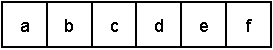
\includegraphics[width=0.35\linewidth]{01_introducao/rep_ga.pdf}
\caption{Um exemplo de indivíduo representado por uma sequência de caracteres com tamanho fixo.}
\label{fig:intro-repga}
\end{figure}

Para muitos problemas a representação natural de uma solução é um programa hierárquico de tamanho variável, ao invés de uma estrutura de comprimento fixo. Isso ocorre porque, frequentemente, não se sabe de antemão as dimensões da solução procurada.

Programas de computador hierárquicos, particularmente escritos em linguagens funcionais e/ou recursivas, podem ser facilmente representados por árvores. Por essa razão, linguagens que processam listas são escolhas naturais para abordar a programação genética \cite{koza97bookGp}.

\begin{figure}[!h]
\centering
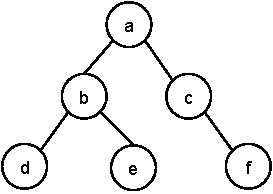
\includegraphics[width=0.4\linewidth]{01_introducao/rep_gp.pdf}
\caption{Representação de um indivíduo na \textit{programação genética}. As letras ``abcdef'' podem representar operações matemáticas, constantes ou até tomadas de decisão.}
\label{fig:intro-repgp}
\end{figure}

A estrutura da Figura \ref{fig:intro-repgp} representa um programa de computador. De fato, é possível escrever funções em LISP utilizando uma representação recursiva semelhante. Programas de computador são entidades capazes de resolver inúmeros problemas em diversos campos, por esse motivo, a programação genética pode ser utilizada em uma gama variada de situações.

Este trabalho busca aplicar a \textit{programação genética} (PG) em problemas clássicos de controle (\ref{fig:intro-gymexemplo}). O sistema do pêndulo invertido da Figura \ref{fig:intro-pendinv} é um dos problemas mais importantes na teoria de controle, principalmente pela sua natureza não-linear e instável, portanto, servirá como estudo de caso básico para este trabalho. O objetivo consiste em balancear o pêndulo utilizando a força $F$ como variável de controle, podendo esta ser aplicada na direção positiva ou negativa do eixo $x$.

\begin{figure}[!h]
\centering
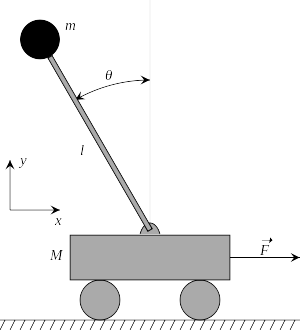
\includegraphics[width=0.4\linewidth]{01_introducao/pend_inv.png}
\captionsource{Pêndulo invertido.}{\url{https://en.wikipedia.org/wiki/Inverted_pendulum}}
\label{fig:intro-pendinv}
\end{figure}

Para realizar a avaliação dos indivíduos, é necessário uma ferramenta de simulação. Foi utilizada a biblioteca \textit{Gym} \cite{openaigym} da linguagem de programação \textit{Python}. O principal propósito desta biblioteca é criar um ambiente padronizado para testar algoritmos de aprendizagem por reforço, porém será utilizada em um problema a ser solucionado por programação genética.

\begin{figure}[H]
\centering
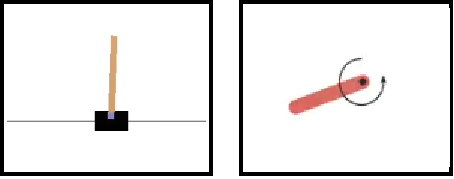
\includegraphics[width=0.5\linewidth]{01_introducao/gym_ex.pdf}
\captionsource{A biblioteca \textit{Gym} fornece alguns problemas de controle clássico como o pêndulo invertido (esquerda) e o pêndulo \textit{swingup}.}{\cite{openaigym}}
\label{fig:intro-gymexemplo}
\end{figure}

A biblioteca DEAP (\textit{Distributed Evolutionary Algorithms in Python}) é um framework de computação evolucionária designada para implementação eficiente de algoritmos evolutivos \cite{deap}. O objetivo é implementar um algoritmo de programação genética utilizando a biblioteca DEAP e evoluir a solução através do ambiente de simulação proporcionado pela biblioteca Gym.

Este trabalho busca uma abordagem didática para a implementação da \textit{programação genética} utilizando ferramentas contemporâneas. Por ser direcionado principalmente a algoritmos de \textit{aprendizagem por reforço}, existem poucas implementações de PG nos ambientes de aprendizado providos pela biblioteca Gym.

Inicialmente, é feita uma análise mais detalhada do ciclo evolutivo artificial, no contexto da programação genética. Além disso, uma verificação detalhada da representação da Figura \ref{fig:intro-repgp} e seus componentes é exigida. Então, aprofunda-se o estudo do pêndulo invertido, buscando formas de incluir na representação dos indivíduos informações importantes para a resolução do problema.

Com o modo de representação dos indivíduos definido, pode-se pensar em como inicializá-los. O conjunto de ferramentas DEAP proporciona diversos métodos que simplificam este processo. Aborda-se, então, maneiras de verificar a aptidão dos indivíduos, que representa, em suma, o desempenho de cada solução encontrada ao longo da execução do algoritmo.

Com uma medida de desempenho atribuída a cada indivíduo, pode-se implementar um método para selecionar indivíduos com base em sua aptidão. São discutidas as possíveis abordagens para essa etapa. Finalmente, as operações genéticas são implementadas em seguida.

% desenvolvimento
\section{A PROGRAMAÇÃO GENÉTICA}\label{sec:1pg-apg}

Um breve sumário da programação genética foi incluído na Introdução. Entretanto, é preciso aprofundar os conceitos mencionados. Neste capítulo são abordados os aspectos mais específicos da representação da Figura ~\ref{fig:intro-repgp}, isto é, o que exatamente são os caracteres $abcdef$ em cada problema. Uma visão geral do ciclo evolutivo artificial é incluída neste capítulo, e servirá de base para os próximos, já que o objetivo é implementar o algoritmo completo.

A aprendizagem evolucionária, em geral, pode ser sumarizada com etapas semelhantes às apresentadas na Figura \ref{fig:1pg-ciclosimples}.

\begin{figure}[!htb]
\centering
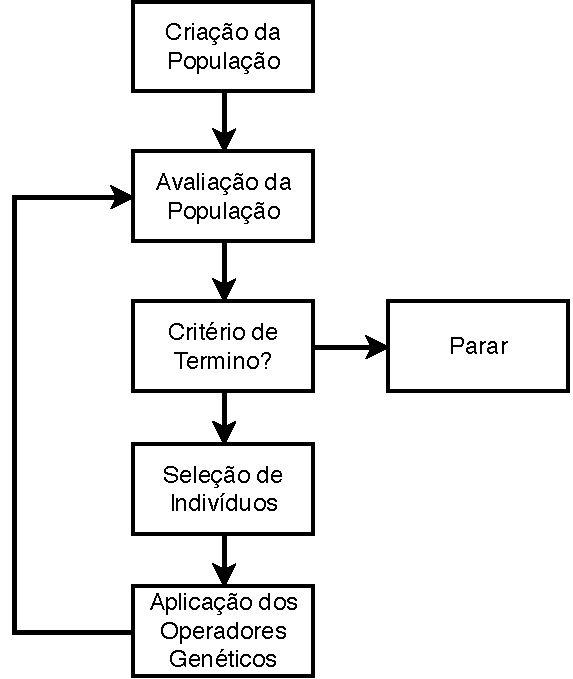
\includegraphics[width=0.4\linewidth]{02_desenvolvimento/01_Pg_Fig_ExCicloSimples}
\caption{Aprendizagem evolucionária.}\label{fig:1pg-ciclosimples}
\end{figure}

O primeiro passo é a criação da população de indivíduos, de acordo com a representação escolhida. A abordagem deste trabalho utiliza o conceito proposto por Koza~\cite{koza92bookGp}, onde cada indivíduo possui uma estrutura recursiva (semelhante a uma árvore) que representa, em sua essência, um programa de computador.

Para os problemas que serão abordados, em suma, o objetivo é encontrar uma lei de controle capaz de estabilizar o sistema ou alcançar um propósito definido. Por exemplo, um indivíduo aleatório inicializado poderia ter uma estrutura igual à apresentada na Figura \ref{fig:1pg-exrepresentacao}. A lei de controle seria dada pela expressão matemática que resulta do cálculo recursivo da árvore que representa o indivíduo.

\begin{figure}[!htb]
\centering
\includegraphics[width=0.4\linewidth]{02_desenvolvimento/01_Pg_Fig_ExRepresentacao.png}
\caption{Um indivíduo aleatório representando uma lei de controle. $c_1$ e $c_2$ são constantes. $s_1$ e $s_2$ são leituras de um sensor.}\label{fig:1pg-exrepresentacao}
\end{figure}

Na Figura \ref{fig:1pg-exrepresentacao}, círculos representam \textbf{operadores}, enquanto os quadrados, \textbf{variáveis terminais}. Como a representação utilizada se assemelha à uma árvore, é possível definir como:

\begin{itemize}[label=\raisebox{0.25ex}{\tiny$\bullet$}]
	\item \underline{Raiz:} o operador do topo (i.e., que não é argumento de outro operador).
	\item \underline{Ramo:} a estrutura composta por um operador e seus argumentos (mesmo que estes sejam outros ramos).
	\item \underline{Folha:} a variável terminal, isto é, uma constante ou uma variável. Caracteriza-se por não ser operador e, portanto, não possui argumentos.
\end{itemize}

Os operadores podem ser matemáticos ou lógicos. Quanto à aridade, pode-se utilizar operadores que aceitem um ou mais argumentos. As variáveis terminais podem ser constantes como $1$ e $0$ ou até números aleatórios dentro de uma faixa. Em problemas de controle é comum admitir como variáveis terminais uma leitura de sensor, por exemplo.

Em linguagens de programação baseadas no processamento de listas, o indivíduo da Figura \ref{fig:1pg-exrepresentacao} poderia ser descrito através da expressão:

\begin{equation*}
(+(*(s_1)(c_1))(-(s_1)(\cos(c_2))))
\end{equation*}

Geralmente, a representação em forma de árvore é mais intuitiva. Entretanto, costuma ser mais eficiente trabalhar com sequências de caracteres, representando uma lista.

É possível estipular, também, um tamanho mínimo e máximo de cada árvore, eliminando assim expressões muito simples, em que sabemos não servir como solução para o problema, ou soluções demasiadamente complexas.

Existem diversas variações da estrutura em forma de árvore. Na programação genética cartesiana~\cite{miller08Cgp}, por exemplo, cada variável de entrada pode servir de operando para mais de um operador. Na programação genética linear~\cite{douglas05Pgl}, um indivíduo é um programa de computador com instruções independentes, executadas de forma sequencial.

A inicialização de cada indivíduo é feita de forma aleatória, respeitando um dado conjunto de operadores $\mathcal{O}$, variáveis terminais $\mathcal{V}$ e nível (ou número de camadas) $\mathcal{D} \in (D_{min}, D_{max})$.

Por exemplo, se definirmos:

\begin{align}
\label{eq:1pg-caractexpopinicial}
\mathcal{O} &= \{+, -, *\} \nonumber\\
\mathcal{V} &= \{1, 0, 3\}\\
\mathcal{D} &= \{1, 2\} \nonumber
\end{align}

Indivíduos como os da Figura \ref{fig:1pg-expopinicial} seriam possíveis elementos dessa população.

\begin{figure}[!htb]
\centering
\includegraphics[width=0.8\linewidth]{02_desenvolvimento/01_Pg_Fig_ExInicializacao.png}
\caption{Um exemplo de inicialização de uma população de três indivíduos, com as características descritas na Equação \ref{eq:1pg-caractexpopinicial}.}\label{fig:1pg-expopinicial}
\end{figure}

Após a inicialização da população é feita a avaliação de cada indivíduo. O objetivo desta etapa é verificar a aptidão de todos os membros da população, através de uma medida que reflita o que se busca como solução para o problema, ou seja, a função que determina o desempenho da solução é específica a cada aplicação.

Em problemas de controle, geralmente o objetivo é manter a posição de um objeto o mais próximo possível de um valor de referência, $X_{ref}$, utilizando uma medição do valor atual, $X_{med}$. Diagramas como o da Figura \ref{fig:1pg-malhacontroleclassico} são comuns na teoria clássica de controle.

\begin{figure}[H]
	\centering
	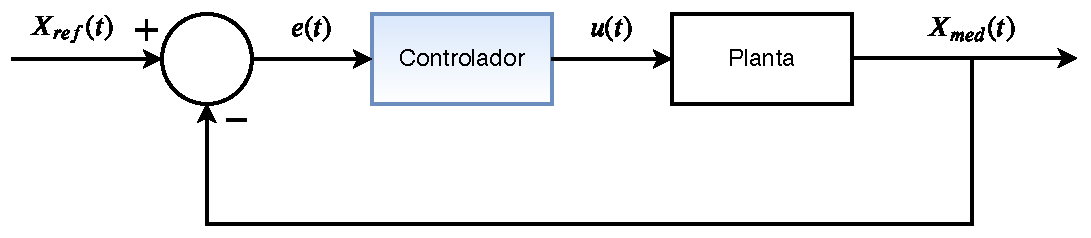
\includegraphics[width=0.85\linewidth]{02_desenvolvimento/01_Pg_Fig_MalhaControleClassico.pdf}
	\caption{Sistema de controle por realimentação. O sinal de erro, $\bm{e(t)}$, é a entrada do controlador, que atua na planta através do sinal de controle, $\bm{u(t)}$.}
	\label{fig:1pg-malhacontroleclassico}
\end{figure}

A avaliação de um indivíduo pode ser representada como uma função custo, $\mathbf{J}$. O objetivo do algoritmo é, portanto, achar um sinal de controle que minimiza $\mathbf{J}$, uma métrica que leva em consideração o erro $e(t)$, em um intervalo de tempo.

% Uma função custo é implementada de modo que penalize desvios de um estado de referência, conforme indica a Equação \ref{eq:1pg-funcaoCusto}.

\begin{equation}\label{eq:1pg-funcaoCusto}
J = \dfrac{1}{T}\int_0^{T}j(e(t))\,dt = \dfrac{1}{T}\int_0^T\left(X_{ref}-X_{med}\right)^2\,dt
\end{equation}

Na programação genética, o indivíduo age como o controlador da Figura \ref{fig:1pg-malhacontroleclassico}, porém, recebe apenas uma medida do estado atual para guiar sua atuação. Isto é, o erro é utilizado apenas por um processo externo à interação do indivíduo com a planta, como um meio de realizar o cálculo de $\mathbf{J}$. Este, por sua vez, é um valor que pode representar a aptidão deste indivíduo. Este processo pode ser observado na Figura \ref{fig:1pg-malhacontrolepg}.

\begin{figure}[H]
	\centering
	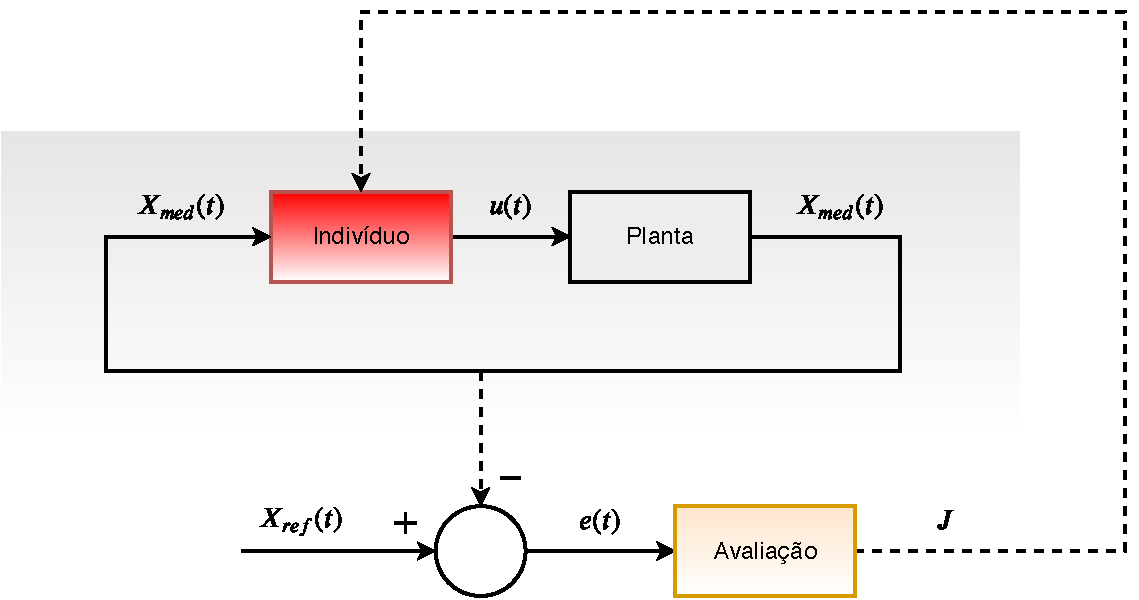
\includegraphics[width=0.85\linewidth]{02_desenvolvimento/01_Pg_Fig_MalhaControlePG.pdf}
	\caption{O indivíduo interage com a planta utilizando apenas medições do estado atual do sistema.}
	\label{fig:1pg-malhacontrolepg}
\end{figure}

Com uma medida de aptidão associada a cada indivíduo, é possível selecionar os mais aptos. Um método básico e eficaz de seleção é comparar dois indivíduos aleatórios na população, utilizando a métrica de desempenho estipulada, e escolher o que possui maior valor numérico de aptidão.

Esse método conhecido como \textit{torneio} pode ser feito em dois ou mais níveis, isto é, são escolhidos quatro ou mais indivíduos aleatórios na população, realizando comparações dois a dois, de modo que apenas um indivíduo seja escolhido ao final.

Um dos operadores genéticos é aplicado neste indivíduo e a solução gerada é inserida em uma nova população. O processo de seleção, aplicação de operadores genéticos e eventual inserção do indivíduo se repete até que o número de indivíduos gerados seja igual a quantidade de membros da população antiga.

Para cada indivíduo selecionado, apenas uma operação genética é aplicada, após ser escolhida de forma aleatória. Cada operação genética tem, portanto, uma probabilidade de ser selecionada. A soma das probabilidades de cada operação deve ser igual a um.

%\begin{itemize}[label=\raisebox{0.25ex}{\tiny$\bullet$}]
% \item $P_c$: probabilidade de cruzamento.
% \item $P_m$: probabilidade de mutação.
% \item $P_r$: probabilidade de replicação.
%\end{itemize}

\begin{equation}
\left.\begin{aligned}
P_c&\text{: probabilidade de cruzamento} \\
P_m&\text{: probabilidade de mutação} \\
P_r&\text{: probabilidade de replicação}
\end{aligned}\right\} P_c+P_m+P_r=1
\end{equation}

É interessante lembrar que o ciclo evolutivo é uma \textbf{busca} por soluções. Nesse contexto, são comuns na literatura os termos \textbf{exploration} e \textbf{exploitation}, que se referem a exploração, entretanto \textit{exploration} se refere a uma busca em larga escala, enquanto \textit{exploitation} refere-se a uma procura local.

De acordo com Brunton et al. \cite{duriez17bookMlc}, a procura pelo mínimo da função custo pode ser representada por gráficos semelhantes ao da Figura \ref{fig:1pg-grafbuscaexpl}, onde a operação de cruzamento realiza uma busca local (exploitation), enquanto a mutação opera em larga escala (exploration).


\begin{figure}[!!htb]
\centering
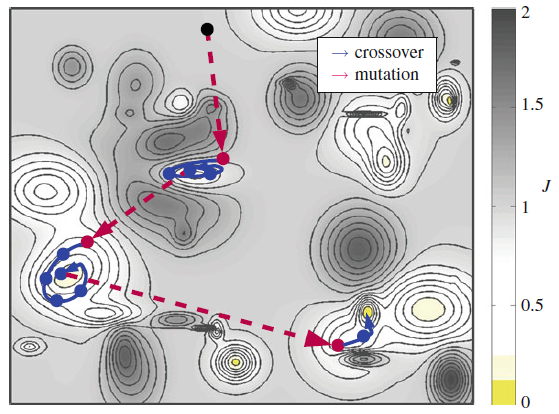
\includegraphics[width=0.7\linewidth]{02_desenvolvimento/01_Pg_Fig_GraficoBuscaExploration.png}
\captionsource{Representação 2D da busca pelo mínimo da função custo. A operação de mutação permite uma busca em larga escala (em vermelho). Em azul, a operação de cruzamento busca a convergência para o mínimo local.}{\cite{duriez17bookMlc}}\label{fig:1pg-grafbuscaexpl}
\end{figure}

A operação de cruzamento, demonstrada na Figura \ref{fig:1pg-excruzamento}, é realizada em dois indivíduos selecionados, isto é, aptos de acordo com o critério de desempenho escolhido. É razoável, portanto, que seja responsável pela convergência local, pois os novos indivíduos gerados possuem \textbf{toda} sua estrutura formada por ramos de soluções consideradas boas. Já no caso da mutação, o novo indivíduo possuirá uma parcela de sua estrutura sendo gerada de forma aleatória, o que não garante convergência, porém é útil para explorar o espaço de possíveis soluções.

A operação genética de \textit{mutação} começa ao selecionar um ponto aleatório na árvore, podendo este ser interno ou externo (operadores ou variáveis terminais). A mutação remove este ramo (ou folha) e uma nova sub-árvore é gerada aleatoriamente, produzindo uma variável terminal (Figura \ref{fig:1pg-exmutvarterm}) ou um ramo (Figura \ref{fig:1pg-exmutramo}).

\begin{figure}[H]
\centering
\includegraphics[width=1\linewidth]{02_desenvolvimento/01_Pg_Fig_ExMutacaoVarTerm.png}
\caption{Mutação aplicada à um ponto correspondente a uma variável terminal gerando um \textit{ramo}.}\label{fig:1pg-exmutvarterm}
\end{figure}

\begin{figure}[H]
\centering
\includegraphics[width=0.9\linewidth]{02_desenvolvimento/01_Pg_Fig_ExMutacaoRamo.png}
\caption{Mutação aplicada em um ponto correspondente a um \textit{ramo}. A nova sub-árvore possui apenas uma \textit{variável terminal}.}\label{fig:1pg-exmutramo}
\end{figure}

A operação de \textit{cruzamento} atua a partir de dois indivíduos selecionados. Assim como na operação de \textit{mutação}, um ponto aleatório na árvore de cada indivíduo é escolhido aleatoriamente e os ramos correspondentes são trocados entre as soluções (Figura \ref{fig:1pg-excruzamento}).

\begin{figure}[H]
\centering
\includegraphics[width=0.8\linewidth]{02_desenvolvimento/01_Pg_Fig_ExCruzamento.png}
\caption{Exemplo da operação de cruzamento atuando em dois indivíduos.}\label{fig:1pg-excruzamento}
\end{figure}

A \textit{replicação} é um operador genético simples em que um indivíduo selecionado é copiado diretamente para a próxima geração, sem qualquer alteração em sua estrutura, conforme indica a Figura \ref{fig:1pg-exreplicacao}.

\begin{figure}[H]
\centering
\includegraphics[width=0.9\linewidth]{02_desenvolvimento/01_Pg_Fig_ExReplicacao.png}
\caption{Operação de \textit{replicação} aplicada em um indivíduo selecionado.}\label{fig:1pg-exreplicacao}
\end{figure}

Koza~\cite{koza92bookGp} menciona outras operações genéticas como a \textit{edição}, cuja função é editar e simplificar as expressões das árvores; \textit{Permutação}, uma generalização do operador de inversão aplicado em algoritmos genéticos de representações fixas; \textit{Encapsulamento}, um método de identificação de ramos úteis que podem ser referenciados e \textit{elitismo}, que copia os indivíduos de maior aptidão diretamente para a próxima geração.

Geralmente, o critério de término do ciclo evolutivo é um número limite de gerações. Alguns problemas permitem a criação de um critério de desempenho, isto é, o ciclo evolutivo se repete até que um indivíduo obtenha um determinado valor de aptidão.

Uma implementação de programação genética não se torna completa sem o estabelecimento de alguns parâmetros de controle, como por exemplo, o número de indivíduos da população ou a probabilidade de cada operação genética. Os principais parâmetros da PG são enumerados a seguir:

\begin{enumerate}
\item \textbf{Em relação à população:}
\begin{enumerate}[label={\alph*)}]
\item Número de indivíduos da população: $M$
\item Número máximo de gerações: $G$
\item Método de inicialização
\item Método de seleção de indivíduos
\end{enumerate}
\item \textbf{Em relação à representação do indivíduo:}
\begin{enumerate}[label={\alph*)}]
\item Conjunto de operações em ramos: $\mathcal{O}$
\item Conjunto de variáveis terminais: $\mathcal{V}$
\item Mínima profundidade inicial da árvore: $D_{min}$
\item Máxima profundidade inicial da árvore: $D_{max}$
\end{enumerate}
\item \textbf{Em relação às operações genéticas:}
\begin{enumerate}[label={\alph*)}]
\item Probabilidade de cruzamento: $P_c$
\item Probabilidade de mutação: $P_m$
\item Probabilidade de replicação: $P_r$
\end{enumerate}
\end{enumerate}

A partir dos parâmetros estabelecidos e dos métodos esclarecidos neste capítulo, é possível reformular o ciclo da Figura \ref{fig:1pg-ciclosimples} para a inclusão de outros detalhes.

\begin{figure}[!h]
\centering
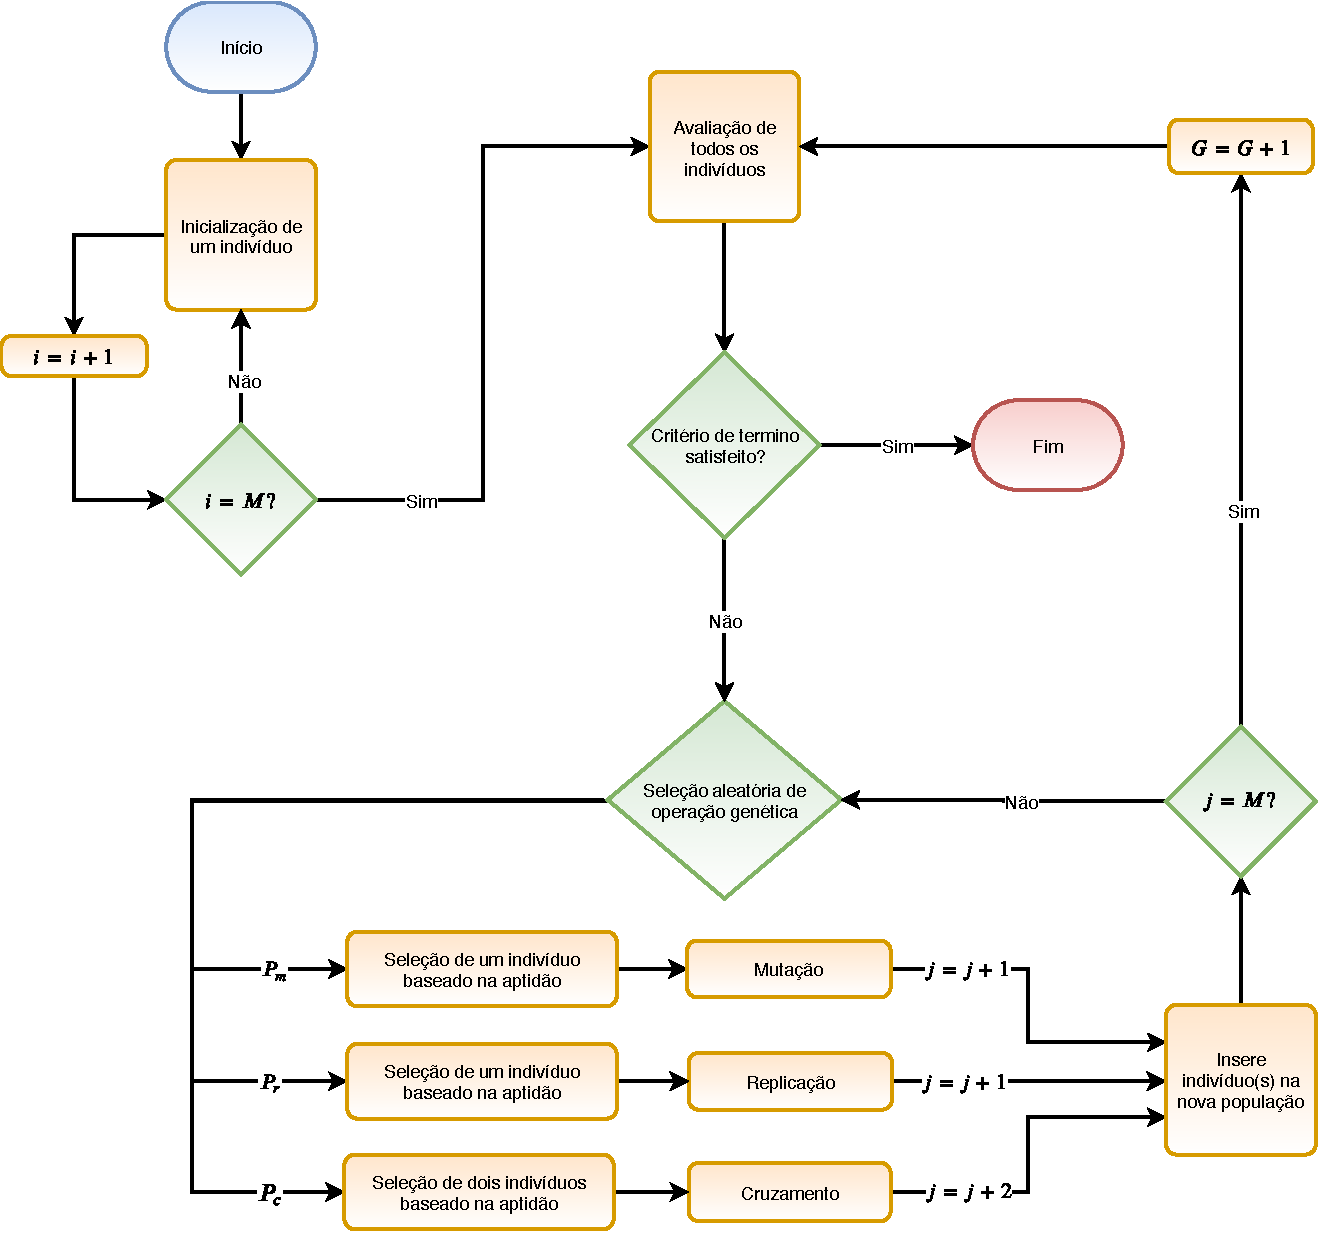
\includegraphics[width=1\linewidth]{02_desenvolvimento/01_Pg_Fig_CicloCompleto.pdf}
\caption{Ciclo evolucionário para programação genética.}\label{fig:1pg-ciclocompleto}
\end{figure}

Com base no fluxograma da Figura \ref{fig:1pg-ciclocompleto} é possível realizar a programação genética para um problema genérico. Resta, portanto, verificar as particularidades da implementação para cada problema abordado.



\section{SIMULAÇÃO DE SISTEMAS DINÂMICOS}\label{sec:2gym-gymependinv}

Foi mencionada a importância de se analisar o problema em que se deseja aplicar a programação genética. Essa análise permite a escolha da função de avaliação, das variáveis terminais e dos operadores. Ao estudar o pêndulo invertido, é possível verificar como um sistema dinâmico pode ser abordado com a PG.

\subsection{PÊNDULO INVERTIDO}\label{ssec:2gym-sistdin}

O pêndulo invertido pode ser considerado um dos sistemas robóticos mais simples, composto apenas por um corpo rígido e um ponto de rotação. Apesar da sua simplicidade, muitas técnicas padrões, derivadas da teoria de controle, são ineficientes e, por isso, o sistema tem importância considerável na área de controle não-linear~\cite{olfa13PendInv}.

Existem diversas variações desse sistema~\cite{wang11PidIp}. O caso abordado neste trabalho trata de um bastão apoiado sobre um veículo que se movimenta com apenas um grau de liberdade, sendo a sua posição dada pela variável $\mathbf{s}$. O ângulo $\mathbf{\theta}$ representa a inclinação do bastão em relação a uma reta normal à superfície. O controle deve ser exercido por uma força $\mathbf{F}$, aplicada paralelamente à superfície, em qualquer sentido, com a finalidade de manter $\theta\approx 0^{\circ}$.

\begin{figure}[!h]
\centering
\includegraphics[width=0.6\linewidth]{02_desenvolvimento/02_PInv_Fig_CartPole.png}
\caption{Sistema do pêndulo invertido.}\label{fig:2gym-cartpole}
\end{figure}

O sistema de equações diferenciais que modela a dinâmica do problema é descrito na Equação \ref{eq:2gym-sisteq}.

\begin{align}\label{eq:2gym-sisteq}
\ddot{\theta} &= \dfrac{g\sin\theta+\cos\theta\left[
\dfrac{-F-m_cl\dot{\theta}^2\sin\theta+\mu_c\sign{(\dot s)}}{m_c+m_b}\right] - \dfrac{\mu_p\theta}{m_bl}}
{l
\left[\dfrac{4}{3} - \dfrac{m_b\cos^2\theta}{m_c+m_b}
\right]}\nonumber\\\\
\ddot{s} &= \dfrac {F+m_bl\left[ \dot{\theta}^2\sin\theta-\ddot\theta\cos\theta \right]
-\mu_c\sign(\dot s)}
{m_c+m_b}\nonumber
\end{align}

Onde:

\begin{itemize}[label=\raisebox{0.25ex}{\tiny$\bullet$}]
\item $g$ = -9,8 \si{m/s^2}, aceleração causada pela gravidade;
\item $m_c$ = 1,0 \si{kg}, massa do carro;
\item $m_b$ = 0,1 \si{kg}, massa do bastão;
\item $l$ = 0,5 \si{m}, metade do comprimento do bastão;
\item $\mu_c$ = 0,0005, coeficiente de atrito do carro na superfície;
\item $\mu_p$ = 0,000002, coeficiente de atrito do bastão no carro;
\item $F$ = $\pm$10,0 \si{N}, força aplicada no centro de massa do carro.
\end{itemize}

Barto et al.~\cite{barto83CartPole} utilizam o subscrito $t$ (omitido neste trabalho) para algumas variáveis, com a finalidade de explicitar a dependência do tempo discreto. A Equação \ref{eq:2gym-sisteq} serviu de base para a implementação do ambiente simulado na biblioteca \textit{Gym}~\cite{gymCartPole}.

\subsection{BIBLIOTECA ``OPENAI GYM’’}\label{ssec:2gym-openaigym}

Antes de discutir a implementação do sistema na biblioteca \textit{Gym}, é feita uma análise das suas principais funcionalidades. \textit{Gym} é uma biblioteca voltada principalmente para o teste de algoritmos de aprendizagem por reforço. Frequentemente, os ambientes de aprendizado para esses algoritmos são descritos através de \textit{processos de decisão Markovianos}.

A principal ideia dos sistemas Markovianos é a interação de um \textit{agente} com um \textit{ambiente} externo, através de ações, estados e recompensas, denotados por $A_t$, $S_t$ e $R_t$, respectivamente. A cada passo de tempo, o ambiente fornece ao agente o seu estado atual ($S_t$) e uma recompensa ($R_t$). Uma ação ($A_t$), gerada pelo agente, influenciará o sistema dinâmico no próximo instante. O objetivo do agente é maximizar a expectativa de recompensa acumulada ao longo do tempo, através de suas ações. Este processo é descrito graficamente na Figura \ref{fig:2gym-mdp}.

\begin{figure}[!h]
\centering
\includegraphics[width=0.8\linewidth]{02_desenvolvimento/02_PInv_Fig_Mdp.png}
\captionsource{Processo de decisão de Markov.}{Adaptado de~\cite{sutton18bookRl}.}
\label{fig:2gym-mdp}
\end{figure}

%Para processos Markovianos, um estado $S_t$ caracteriza completamente a dinâmica de um sistema, no instante $t$. Isto significa que para ambientes estocásticos Markovianos, dado um estado $S_t$ e uma ação $A_t$, sabemos a probabilidade associada a cada possível próximo estado, $S_{t+1}$ e recompensa futura $R_{t+1}$. Não há probabilidades associadas ao sistema do pêndulo invertido, logo, para o nosso problema, se há um estado Markoviano $S_t$ observável, saberemos com precisão qual será o próximo estado do sistema e a recompensa futura recebida pelo agente.

Para processos de decisão Markovianos, $R_t$ e $S_t$ são variáveis aleatórias com distribuições de probabilidade que dependem apenas do estado e ação anteriores, $S_{t-1}$ e $A_{t-1}$, respectivamente. Para sistemas determinísticos, como os que são abordados neste trabalho, há um mapeamento $S_t,\,A_t \to S_{t+1}$.

As simulações da biblioteca Gym são baseadas em processos de decisão Markovianos. Portanto, a cada iteração existe uma variável acessível ao agente, que indica o estado atual do ambiente e sua recompensa, $S_t$ e $R_t$, respectivamente. O agente será a máquina que aprende com a experiência, mais especificamente, com informações de estados e recompensas obtidas ao longo do tempo.

% Além disso, vimos que o agente influencia o sistema através de ações $A_t$, cuja implementação também é proporcionada pela biblioteca.

%Estados Markovianos descrevem completamente o próximo estado do ambiente. Por esse motivo, $S_t$ deve conter informações suficientes para que possamos prever o próximo estado. Essa restrição imposta aos estados explica o motivo da observação fornecida ao agente pela biblioteca. Mais especificamente, para o problema do pêndulo invertido, a observação fornecida ao agente inclui as variáveis de estado:

Estados Markovianos devem conter informações suficientes para que, dadas uma ação e uma observação do estado atual, seja possível prever o próximo estado. Desta forma, fica claro que a observação fornecida deve conter dados sobre as variáveis de estado do sistema.

%pois essa informação aliada à entrada gerada pelo agente (força $\mathbf{F}$) é suficiente para indicar o próximo estado.

\begin{table}[!htb]
\centering
\caption{Variáveis de estado fornecidas como observação do estado atual ($S_t)$).}
\label{tab:2gym-observacao}
\begin{tabular}{l|l|l|l} \toprule
{Variável} & {Significado} & {Valor Mínimo} & {Valor Máximo}\\ \midrule
{$s$} & {Posição do carro} & {$-4.8$} & {$4.8$} \\
{$\dot{s}$} & {Velocidade do carro} & {$-\infty$} & {$\infty$} \\
{$\theta$} & {Ângulo do bastão} &{$\SI{-24}{\degree}$} & {$\SI{24}{\degree}$} \\
{$\dot\theta$} & {Velocidade angular do bastão} & {$-\infty$} & {$\infty$}
\\ \bottomrule
\end{tabular}
\end{table}

A simulação ocorre em episódios de duração limitada: o término acontece quando as variáveis de estado ou o tempo decorrido excedem um certo valor, conforme exemplifica a Tabela 1.

A implementação de recompensas ($R_t$) no ambiente do pêndulo invertido é simples: a cada instante de tempo, o agente recebe $1$ de recompensa. Controladores com baixo desempenho irão forçar o término do episódio rapidamente, recebendo pouca recompensa. 

Os componentes da simulação estão implementados na linguagem de programação \textit{Python}, utilizando classes e categorias de dados específicos.

\begin{figure}[H]
\centering
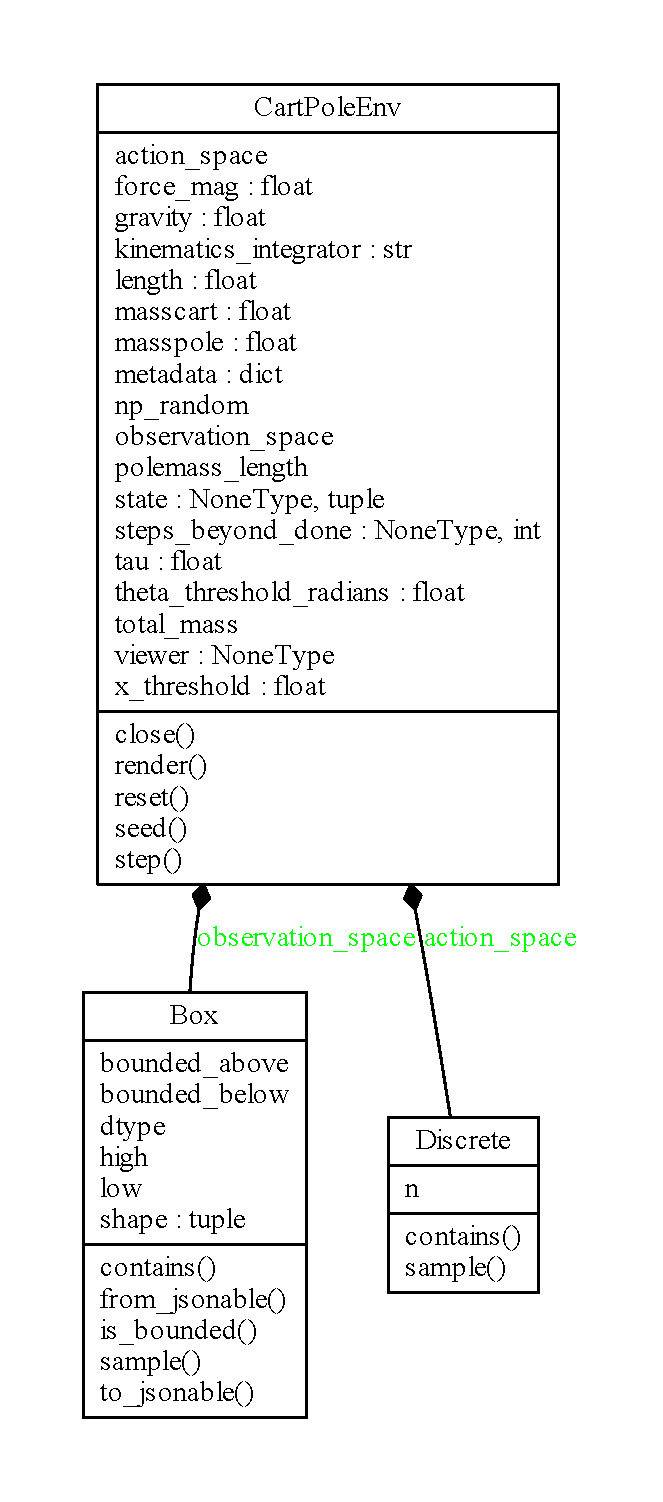
\includegraphics[width=0.5\linewidth]{02_desenvolvimento/02_PInv_Fig_ClassUML.pdf}
\caption{Diagrama de classes para o ambiente de simulação do pêndulo invertido, gerado com o utilitário \textit{pyreverse}.}\label{fig:2gym-umlclasse}
\end{figure}

Na Figura \ref{fig:2gym-umlclasse}, é possível verificar que os objetos \textit{observation\_space} e \textit{action\_space} pertencem às classes \textit{Box} e \textit{Discrete}, respectivamente, e compõem o ambiente de simulação. Essas classes determinam quais são as observações e ações possíveis na simulação, isto é, impõe restrições às ações que o agente pode tomar e à observação recebida. Na simulação do pêndulo invertido, as ações estão restritas aos valores inteiros $0$ e $1$, por exemplo, indicando a aplicação da força para a esquerda ou para a direita. Os métodos disponíveis são utilizados para realizar a interação do agente com o ambiente. As principais funções existentes são detalhadas a seguir:

\begin{enumerate}[label=\alph*)]
\item \textbf{\underline{make(\textit{nome})}}:
\begin{itemize}[label=\raisebox{0.25ex}{\tiny$\bullet$}]
\item \textbf{Descrição}: cria um objeto em que ocorre a simulação.
\item \textbf{Argumento}: (\textit{String}) nome do ambiente de simulação. Ex: 'CartPole-v1'
\item \textbf{Retorno}: (\textit{Env}) Ambiente de simulação.
\end{itemize}
\item \textbf{\underline{reset(\textit{ambiente})}}:
\begin{itemize}[label=\raisebox{0.25ex}{\tiny$\bullet$}]
\item \textbf{Descrição}: inicia um episódio de simulação, com valores iniciais aleatórios dentro de uma faixa específica.
\item \textbf{Argumento}: (\textit{Env}) o objeto (ambiente de simulação) que será inicializado.
\item \textbf{Retorno}: (\textit{Box}) observação (objeto) que contém o valor das variáveis de estado.
\end{itemize}
\item \textbf{\underline{step(\textit{ambiente}, \textit{ação})}}:
\begin{itemize}[label=\raisebox{0.25ex}{\tiny$\bullet$}]
\item \textbf{Descrição}: realiza a \textit{ação} no sistema.
\item \textbf{Argumento}: (\textit{Env}, \textit{Int}) objeto com o ambiente de simulação e ação discreta do agente.
\item \textbf{Retorno}: (Tupla) uma tupla que contém: observação (após a ação do agente), recompensa, indicação de término do episódio e informações adicionais.
\end{itemize}
\item \textbf{\underline{render(\textit{ambiente}, \textit{modo})}}:
\begin{itemize}[label=\raisebox{0.25ex}{\tiny$\bullet$}]
\item \textbf{Descrição}: renderiza o ambiente de simulação.
\item \textbf{Argumento}: (\textit{Env, String}) ambiente a ser simulado e o modo de exibição.
\item \textbf{Retorno}: objeto de renderização.
\end{itemize}
\end{enumerate}

As funções descritas são métodos que atuam no ambiente de simulação. A utilização dessas funções pode ser exemplificada no fluxograma da Figura \ref{fig:2gym-ciclogym}.

\begin{figure}[H]
\centering
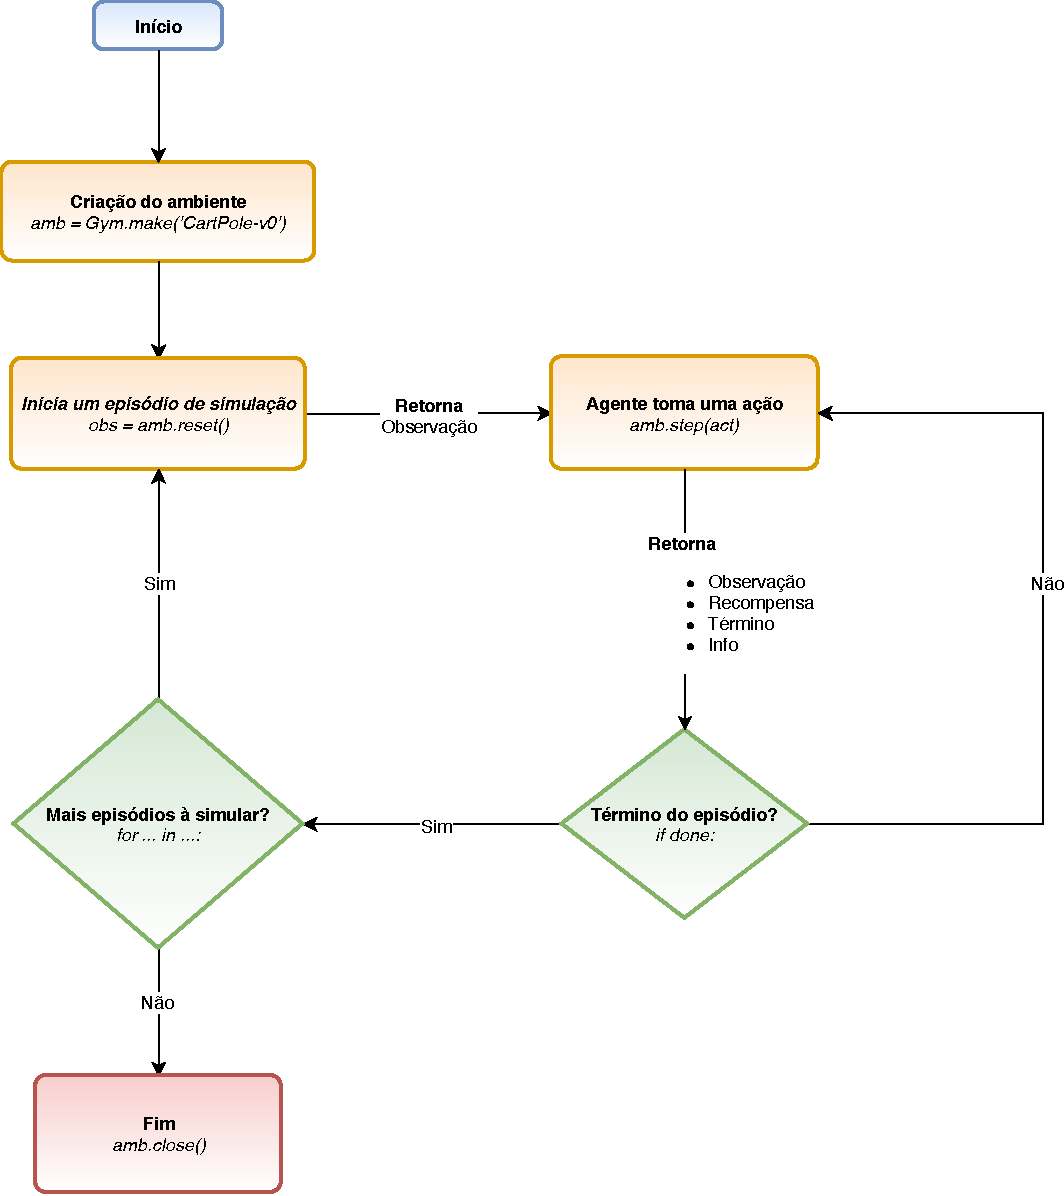
\includegraphics[width=1\linewidth]{02_desenvolvimento/02_PInv_Fig_CicloGym.pdf}
\caption{Forma geral de um algoritmo para realização de uma simulação no \textit{OpenAi Gym}.}\label{fig:2gym-ciclogym}
\end{figure}

É realizado, a seguir, uma análise breve de cada objeto da interação demonstrada na Figura \ref{fig:2gym-ciclogym}, com o objetivo de facilitar a criação do algoritmo.

O principal objeto é o retornado pela função \textit{step}. Trata-se de uma tupla de quatro objetos, os quais o agente utilizará para obter informações sobre o sistema, quais sejam:

\begin{itemize}[label=\raisebox{0.25ex}{\tiny$\bullet$}]
\item \textit{Observação}: lista indexável (Figura \ref{fig:2gym-observacao}) que contém o valor das variáveis de estado do sistema logo após a \textit{ação} do agente.
\begin{figure}[H]
\centering
\includegraphics[width=0.6\linewidth]{02_desenvolvimento/02_PInv_Fig_Observacao.png}
\caption{\textit{Box} é uma classe que permite a criação de conjuntos multidimensionais, no ambiente do pêndulo invertido é apenas uma lista (unidimensional).}\label{fig:2gym-observacao}
\end{figure}
\item \textit{Recompensa}: valor retornado pelo sistema após ter sofrido uma \textit{ação} do agente. Pode apresentar os valores $0$ ou $1$, para o ambiente do pêndulo invertido (Figura \ref{fig:2gym-recompensa}).
\begin{figure}[!h]
\centering
\includegraphics[width=0.15\linewidth]{02_desenvolvimento/02_PInv_Fig_Recompensa.png}
\caption{Recompensa recebida pelo agente.}\label{fig:2gym-recompensa}
\end{figure}
\item \textit{Término}: valor lógico (Figura \ref{fig:2gym-termino}) que indica se o episódio de simulação terminou ou não, de acordo com os critérios estabelecidos.
\begin{figure}[!h]
\centering
\includegraphics[width=0.10\linewidth]{02_desenvolvimento/02_PInv_Fig_Termino.png}
\caption{Valor lógico que indica se o episódio terminou ou não.}\label{fig:2gym-termino}
\end{figure}
\item \textit{Info}: fornece informações adicionais sobre a simulação ao programador. Geralmente, é utilizada para \textit{debugging}.
\end{itemize}

Ao longo deste capítulo foi possível estudar a implementação da simulação de sistemas dinâmicos na biblioteca \textit{Gym}. Esta é uma etapa essencial para verificar o desempenho das soluções encontradas ao longo da execução do algoritmo. O próximo capítulo aborda outros aspectos da programação genética, através da biblioteca DEAP.
\section{DEAP: IMPLEMENTAÇÃO DOS AGENTES}\label{sec:3deap-implagentes}

No capítulo anterior, foi abordada a utilização da biblioteca Gym para simular a interação de um sistema com um agente. Neste capítulo, o objetivo é verificar as funcionalidades providas pela biblioteca DEAP e como essas ferramentas foram utilizadas para representar indivíduos de uma população.

DEAP é uma biblioteca em \textit{Python} que promove a criação de protótipos e ideias na área da
computação evolutiva, com mecanismos que permitem a paralelização de tarefas. Suas áreas de aplicação, além da
programação genética, incluem: algoritmos genéticos, estratégias evolucionárias e otimização por enxame de partículas~\cite{deapdocs}.

Como dito, este trabalho, é voltado para a sua aplicação em PG.\@
O objetivo é implementar uma população de indivíduos,
representados como árvores ou listas de tamanho variável, que
representarão leis de controle para um sistema dinâmico.

Este capítulo descreve a implementação da população e dos indivíduos que a compõem, utilizando as ferramentas proporcionadas pela biblioteca. São analisados os parâmetros essenciais para a representação da solução, isto é, o tamanho da população, o número máximo de níveis das árvores, entre outros aspectos. Em seguida, é implementada a avaliação e seleção de indivíduos. Por fim, são definidos os operadores genéticos e o critério de término.

Já que a biblioteca DEAP será abordada ao longo deste capítulo, é proveitoso ter uma
visão geral das funcionalidades de cada módulo da biblioteca, explicitados na Figura~\ref{fig:3deap-modulos}.

\begin{figure}[H]
	\centering
	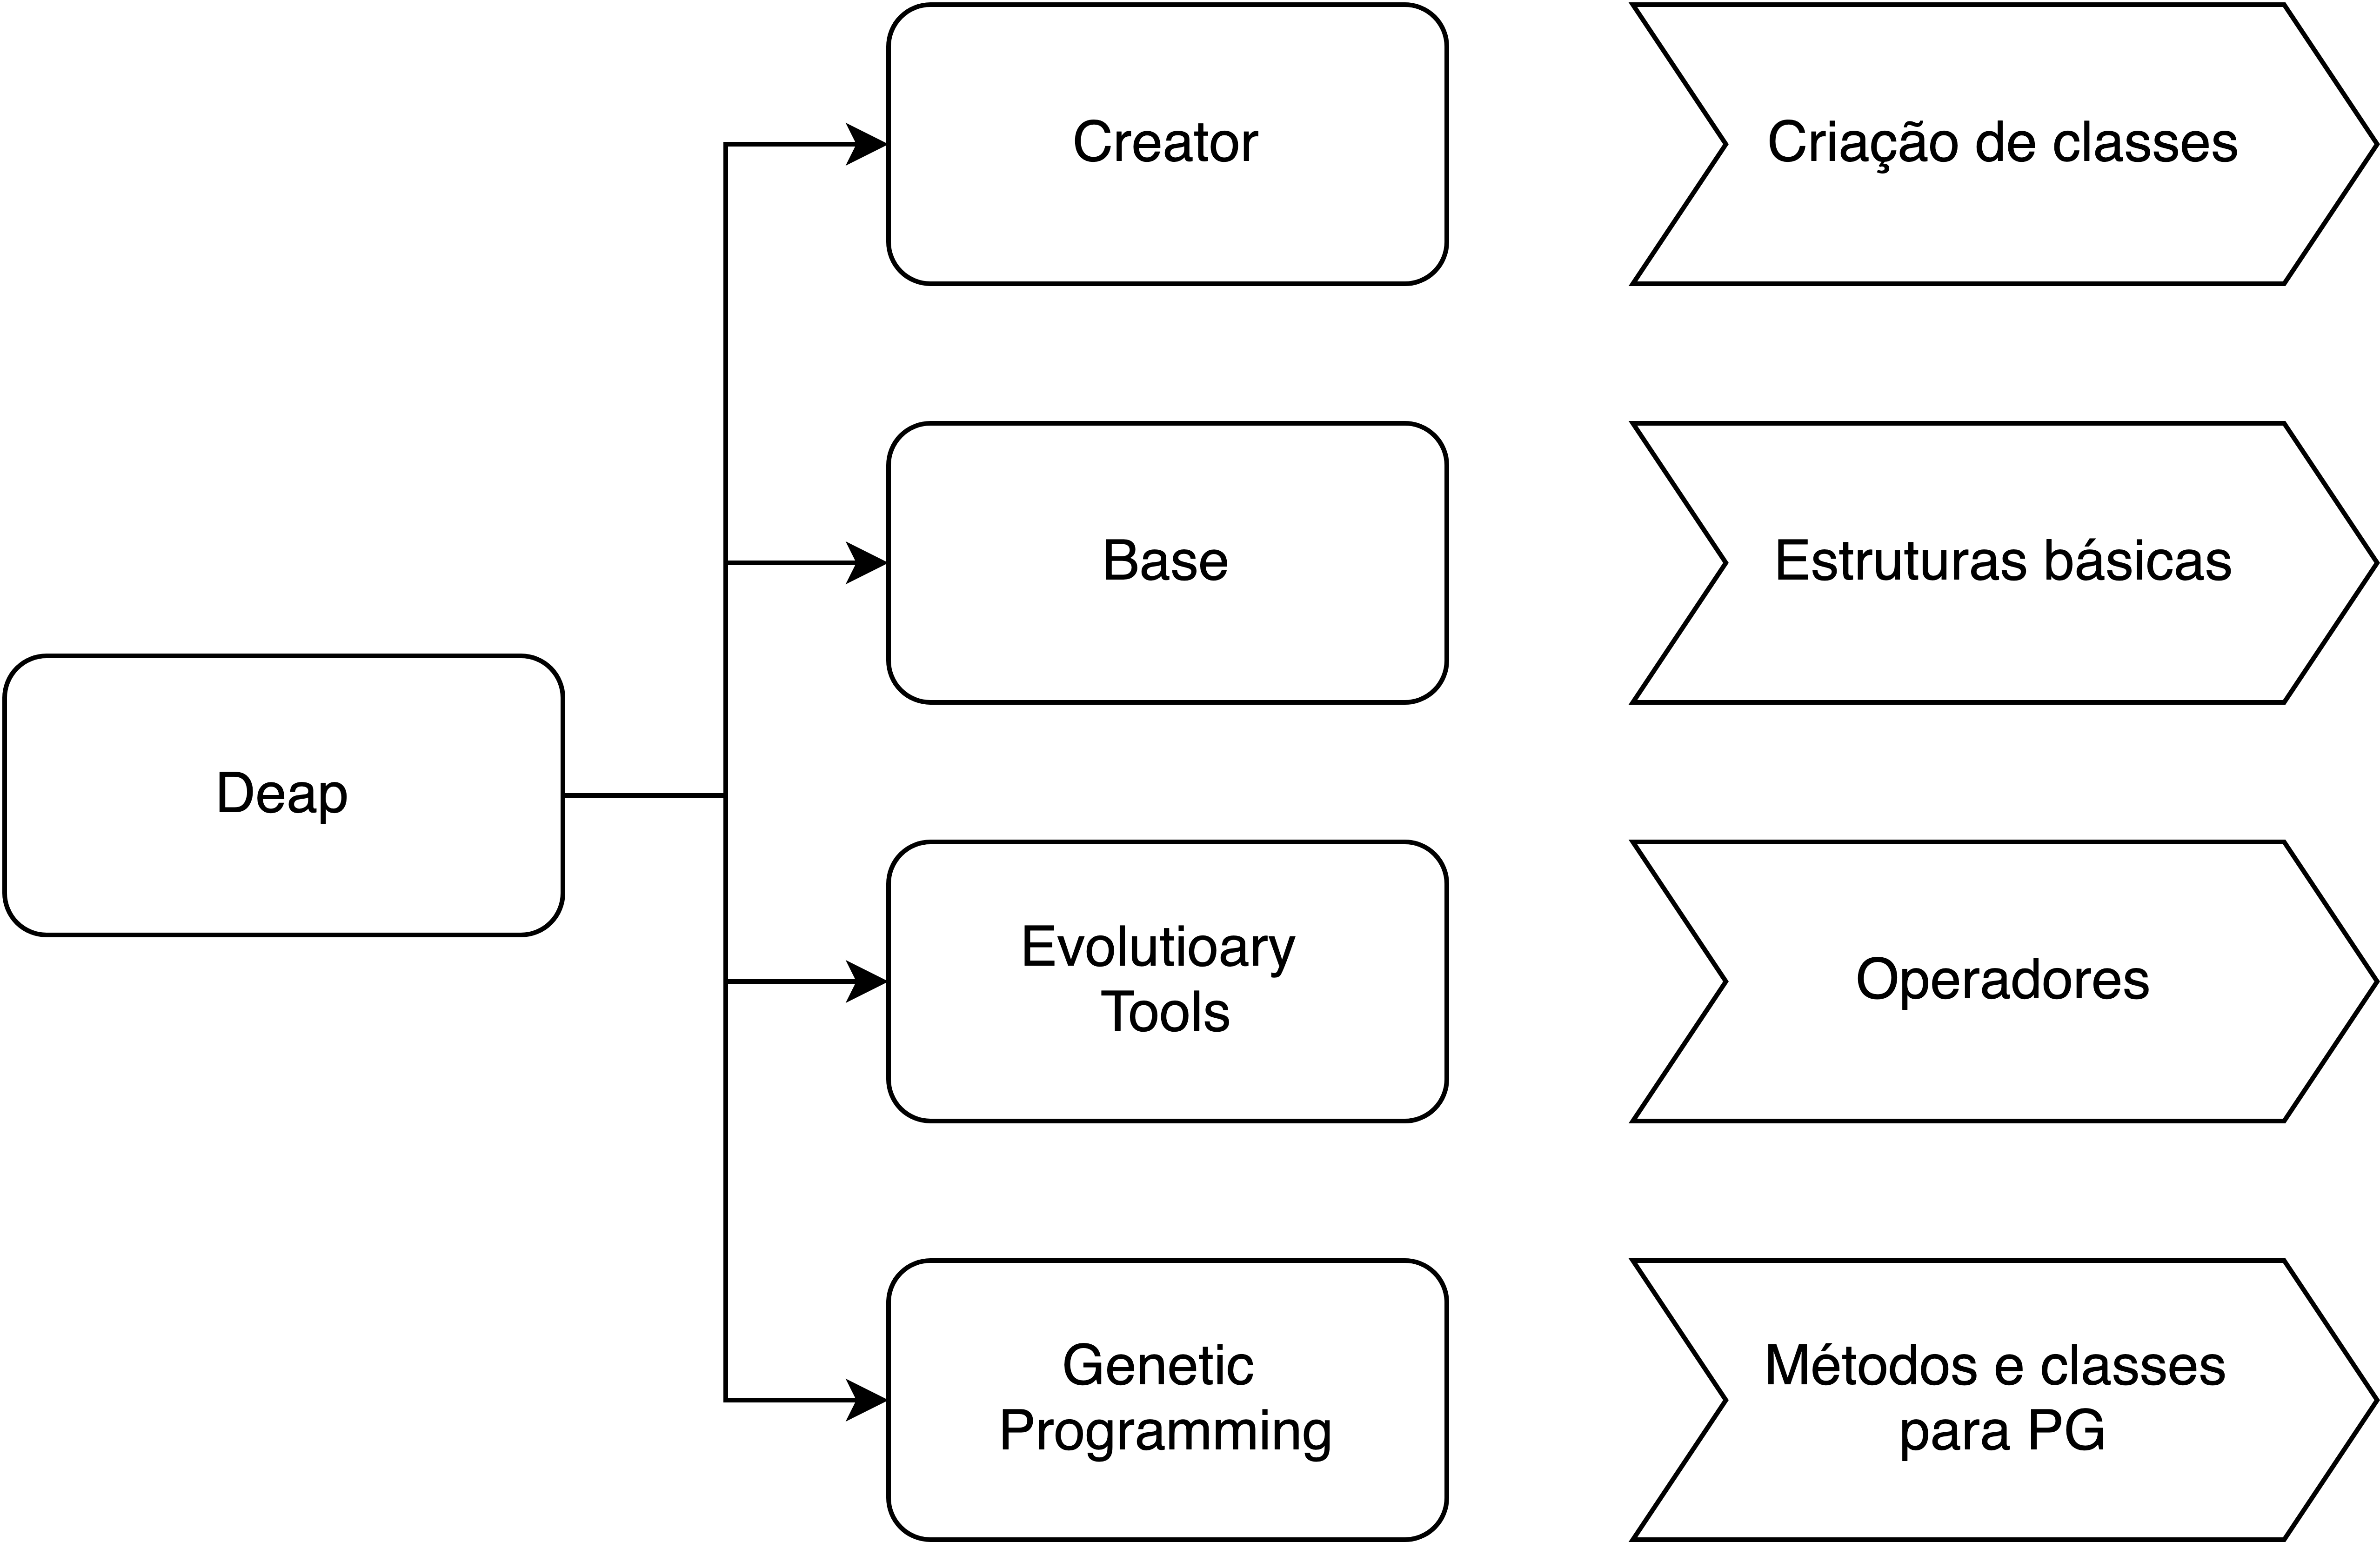
\includegraphics[width=0.7\linewidth]{02_desenvolvimento/03_Deap_Fig_Modulos.png}
	\caption{Módulos da biblioteca DEAP e suas funcionalidades.}\label{fig:3deap-modulos}
\end{figure}

\subsection{REPRESENTAÇÃO E INICIALIZAÇÃO}\label{ssec:3deap-represinic}

No Capítulo \ref{sec:1pg-apg}, a lista dos principais parâmetros que definem uma
implementação de PG é fornecida.\@ Neste capítulo, foi realizado um estudo dos aspectos referentes à representação de cada indivíduo e sua respectiva inicialização, tornando possível a criação de uma população inicial aleatória pronta para sofrer transformações ao longo do ciclo evolutivo.

\subsubsection{Representação}\label{sssec:3deap-representacao}

Para representar um indivíduo na PG deve-se definir: o conjunto de operações e o conjunto de variáveis terminais, denominados por $\mathcal{O}$ e $\mathcal{V}$, respectivamente. Geralmente essas duas entidades são agregadas em único conjunto denominado \textit{primitivo}. Logo, pode-se definir como \textit{conjunto primitivo} $\mathcal{P}$ o grupo que contém todas as funções (de diferentes aridades) e variáveis terminais que compõem os indivíduos da população.

As variáveis terminais podem ser \underline{constantes} ou \underline{entradas} vindas do sistema. As entradas são informações sobre as variáveis de estado do sistema. Geralmente, as constates são valores aleatórios, dentro de uma faixa, gerados na inicialização dos indivíduos. A existência de constantes aleatórias permite uma exploração maior do espaço de buscas, uma vez que as operações que atuam sobre esses números podem moldar coeficientes de uma lei de controle ótima para o problema.

Para o estudo de caso básico (pêndulo invertido), as variáveis terminais utilizadas estão descritas na Tabela \ref{tab:3deap-varterm}.

\begin{table}[H]
	\centering
	\begin{tabular}{l|l|l} \toprule
		{Variável Terminal} & {Significado} & {Tipo}\\ \midrule
		{$s$} & {Posição do carro} & {Entrada}\\
		{$\dot{s}$} & {Velocidade do carro} & {Entrada}\\
		{$\theta$} & {Ângulo do bastão} & {Entrada}\\
		{$\dot{\theta}$} & {Velocidade angular do bastão} & {Entrada}\\
		{$R$} & {Número gerado aleatoriamente ($-1,0<R<1,0$)} & {Constante}
		\\ \bottomrule
	\end{tabular}
	\caption{Variáveis terminais.}\label{tab:3deap-varterm}
\end{table}

Os operadores utilizados estão descritos na Tabela \ref{tab:3deap-operadores}, e foram escolhidos com base na literatura abordada (\cite{duriez17bookMlc}, \cite{koza92bookGp} e \cite{poli08GpFieldGuide}).

\begin{table}[H]
	\centering
	\begin{tabular}{l|l|l|l} \toprule
		\addlinespace[0.4ex] {Operador} & {Símbolo} & {Resultado} & {Aridade}\\ \midrule
		\addlinespace[0.4ex] {Soma} & {$+$} & {$a+b$} & {2} \\
		\addlinespace[0.4ex] {Subtração} & {$-$} & {$a-b$} & {2} \\
		\addlinespace[0.4ex] {Multiplicação} & {$\times$} & {$a\cdot b$} & {2} \\
		\addlinespace[0.4ex] {Divisão} & {$\div$} & {$a/b$} & {2} \\
		\addlinespace[0.4ex] {Raiz Quadrada} & {$\sqrt{}$} & {$\sqrt a$} & {1} \\
		%\addlinespace[0.4ex] {Raiz Cúbica} & {$\sqrt[3]{}$} & {$\sqrt[3] a$} & {1} \\
		\addlinespace[0.4ex] {Seno} & {$\sin$} & {$\cos{(a)}$} & {1} \\
		\addlinespace[0.4ex] {Comparação} & {$>$} & {\makecell{$a$, se $a\ge b$\\$b$, se $a<b$}} & {2} \\
		\addlinespace[0.4ex] {Sinal} & {sgn} & {\makecell{$1$, se $a\ge 0$\\$-1$, se $a<0$}} & {1}
		\\ \bottomrule
	\end{tabular}
	\caption{Conjunto de operadores lógicos e matemáticos.}\label{tab:3deap-operadores}
\end{table}

\begin{table}[H]
	\centering
	\begin{tabular}{l|l|l|l} \toprule
		{Operador} & {Símbolo} & {Resultado} & {Aridade}\\ \midrule
		{Soma} & {$+$} & {$a+b$} & {2} \\
		{Subtração} & {$-$} & {$a-b$} & {2} \\
		{Multiplicação} & {$\times$} & {$a\cdot b$} & {2} \\
		{Divisão} & {$\div$} & {$a/b$} & {2} \\
		{Raiz Quadrada} & {$\sqrt{}$} & {$\sqrt a$} & {1} \\
		%\addlinespace[0.4ex] {Raiz Cúbica} & {$\sqrt[3]{}$} & {$\sqrt[3] a$} & {1} \\
		{Seno} & {$\sin$} & {$\cos{(a)}$} & {1} \\
		{Comparação} & {$>$} & {\makecell{$a$, se $a\ge b$\\$b$, se $a<b$}} & {2} \\
		{Sinal} & {sgn} & {\makecell{$1$, se $a\ge 0$\\$-1$, se $a<0$}} & {1}
		\\ \bottomrule
	\end{tabular}
	\caption{Conjunto de operadores lógicos e matemáticos.}\label{tab:3deap-operadores}
\end{table}

A operação de divisão geralmente é implementada de modo que o denominador possa assumir o valor zero, para evitar possíveis erros durante a execução do programa. Neste caso, o valor retornado será igual a 1.

Um problema se apresenta ao analisar uma possível lei de controle gerada através das funções da Tabela~\ref{tab:3deap-operadores} com as variáveis terminais da Tabela~\ref{tab:3deap-varterm}: os valores que resultam da avaliação da expressão são contínuos. O ambiente do pêndulo invertido impõe uma restrição às ações, através do objeto \textit{action space}. Mais especificamente, estas devem ser valores discretos: $0$ ou $1$.

Já que os indivíduos são expressões matemáticas que produzem resultados numéricos variados, uma possível solução seria definir que a saída produzida será $1$, caso o número produzido na avaliação do indivíduo seja positivo e $0$, caso contrário. Este processo pode ser observado na Figura~\ref{fig:03deap-wrapper}.

\begin{figure}[H]
	\centering
	\includegraphics[width=0.55\linewidth]{02_desenvolvimento/03_Deap_Fig_Wrapper.png}
	\caption{A saída depende do sinal da expressão que resulta da avaliação do indivíduo.}\label{fig:03deap-wrapper}
\end{figure}

Com isso, fica claro que a ação realizada pelo indivíduo está contida
no espaço de ações possíveis, determinado pelo ambiente de simulação.

É necessário agrupar as operações e variáveis
terminais em um conjunto único. O DEAP provê
funcionalidades que permitem a criação de um conjunto primitivo. A
partir da classe \textit{PrimitiveSet} é possível criar tal grupo e incluir funções e variáveis terminais.

\classdef{PrimitiveSet}{name, arity, prefix}{
	Cria um conjunto primitivo de nome \textit{name} com \textit{arity} entradas. Geralmente, \textit{arity} será igual ao número de variáveis fornecidas na observação de estado da simulação. É possível adicionar um prefixo \textit{prefix} à nomeação de cada entrada.}

O nome \textit{main} foi dado ao conjunto primitivo criado, por convenção. Para o problema do pêndulo invertido, por exemplo, a aridade do conjunto primitivo é quatro, isto é, o número de variáveis de estado. É conveniente renomear as entradas alterando o prefixo para facilitar o entendimento (em condições normais, as variáveis da Tabela~\ref{tab:3deap-varterm} seriam nomeadas ARG0, ARG1, ARG2 e ARG3, por exemplo).

Após a criação do conjunto primitivo, a partir da classe descrita, é
possível adicionar a esse objeto as funções da Tabela~\ref{tab:3deap-operadores} e a constante efêmera da Tabela~\ref{tab:3deap-varterm}. As outras variáveis terminais, que correspondem às leituras dos sensores, são definidas como \textbf{entradas} e são adicionadas na
criação do conjunto $\mathcal{P}$.

\metdef{addPrimitive}{op, arity, name}{PrimitiveSet}{
	Adiciona uma operação lógica/matemática \textit{op} ao conjunto primitivo, sob o nome \textit{name}. O parâmetro \textit{arity}, neste caso, define o número de argumentos da função.}

\metdef{addEphemeral}{name, constant}{PrimitiveSet}{Adiciona a
	\textit{constante} ao conjunto primitivo sob o nome \textit{name}.}

A seguir, um atributo de aptidão é adicionado ao indivíduo em sua inicialização.

\subsubsection{Aptidão}\label{sssec:3deap-aptidao}

Ao longo da Capítulo \ref{sec:1pg-apg}, foi visto que existem diversos métodos de representar a aptidão de um indivíduo. Em problemas de controle, é comum expressar esse critério de desempenho como funções custo, semelhantes à Equação \ref{eq:1pg-funcaoCusto}. Um indivíduo apto, portanto, seria caracterizado por um valor baixo de aptidão, ou seja, desejaríamos \underline{minimizar} esta quantidade. Entretanto, seria possível elaborar uma função de aptidão a ser \underline{maximizada}. Para o problema do pêndulo invertido, por exemplo, basta que essa função represente o tempo total do episódio de simulação atingido por um indivíduo. Dessa forma, uma solução com desempenho insatisfatório causaria rapidamente o fim do episódio de simulação (pois o critério de término está relacionado à instabilidade do sistema), e consequentemente, um valor de aptidão baixo seria atribuído a este indivíduo.

O DEAP proporciona uma classe base denominada \textit{Fitness} com um atributo \textit{weight} (peso). O peso indica se a aptidão deve ser maximizada ou minimizada. Um peso positivo, por exemplo, indica que o objetivo do ciclo evolutivo é gerar indivíduos com a aptidão maior possível.

O atributo peso permite facilmente comparar dois indivíduos, pois é possível ignorar a implementação da função de avaliação, ou seja, o maior valor numérico de aptidão indica o indivíduo mais apto, seja o objetivo a maximização ou minimização desta quantidade. Além disso, este componente permite implementar funções de aptidão com múltiplos objetivos.

A biblioteca conta também com uma função de criação de classes, a partir de outras, denominada \textit{create} da biblioteca \textit{creator}.

\fundef{create}{name, base, attributes}{
	Cria a classe com o nome \textit{name} a partir da classe \textit{base} com os atributos adicionais \textit{attributes}.}

Já que o ambiente de simulação proporcionado pela biblioteca Gym provê uma recompensa unitária a cada intervalo de tempo discreto em que o episódio não termina, é possível calcular a aptidão de um indivíduo como a soma de recompensas acumulada ao longo do tempo. Como a busca é por indivíduos com o máximo de aptidão, essa classe pode ser nomeada \textit{AptidaoMax}.

\subsubsection{Inicialização}\label{sssec:3deap-inicializacao}

Os indivíduos de uma população possuem uma estrutura semelhante a uma árvore, cujo conteúdo pertence a um conjunto primitivo de operadores e variáveis terminais e que possuem um atributo de aptidão, que caracteriza o desempenho da solução no sistema. Tais características de um indivíduo foram implementadas nas Seções~\ref{sssec:3deap-representacao} e~\ref{sssec:3deap-aptidao}, restando, portanto, criar uma estrutura de dados que possa ser inicializada de forma aleatória utilizando o conjunto primitivo e que possua um atributo de aptidão.

As principais escolhas associadas a esta etapa estão relacionadas à profundidade das árvores representando os indivíduos e o método de inicialização, ou seja, como essas árvores seriam geradas.

No Capítulo~\ref{sec:1pg-apg} foi definido como $D_{\min}$ a profundidade mínima da árvore que representa um indivíduo inicializado, isto é, que faz parte da população inicial. $D_{\max}$ foi estabelecido como a profundidade máxima de um indivíduo inicializado, ou seja, a maior distância da raiz a uma variável terminal.

Foram escolhidos os valores 2 e 5 para $D_{\min}$ e $D_{\max}$, respectivamente, para o problema do pêndulo invertido. Na Figura \ref{fig:3deap-profundidade} pode-se ver alguns exemplos de indivíduos inicializados com valores extremos de profundidade da árvore.

\begin{figure}[H]
	\centering
	\includegraphics[width=0.6\linewidth]{02_desenvolvimento/03_Deap_Fig_Profundidade}
	\caption{As linhas pontilhadas indicam a maior distância entre a \textit{raiz} e uma \textit{variável terminal}. Este exemplo utiliza o conjunto primitivo $\mathcal{P}$ definido anteriormente.}\label{fig:3deap-profundidade}
\end{figure}

Pode-se notar que uma expressão pode conter diferentes profundidades, com o valor entre os extremos pré-estabelecidos. Por exemplo, na Figura \ref{fig:3deap-profundidade}, o indivíduo da direita possui caminhos com comprimento mínimo apesar de conter um caminho de profundidade máxima. Se partirmos do princípio de que a criação dos indivíduos se inicia a partir da raiz, o que determina a profundidade máxima do indivíduo a ser criado é a escolha: o próximo nó é um operador ou uma variável terminal?

No processo de criação de árvores a partir da raiz, é possível fazer com que todos os caminhos possíveis da árvore sejam o maior possível, $D_{\max}$. Este método de inicialização é chamado de \textit{full}~\cite{koza92bookGp}. Os indivíduos também podem ser gerados com caminhos de comprimento aleatório (dentro da faixa estipulada), isto é: a única restrição é que cada caminho deveria ter um comprimento $l_i$ tal que $D_{\min} \le l_i \le D_{\max}$. Este método é conhecido como \textit{grow}.

Koza~\cite{koza92bookGp} sugere um método híbrido, frequentemente empregado na literatura abordada, denominado \textit{ramped half-and-half}. Nessa abordagem são gerados $N$ indivíduos para cada nível máximo de profundidade $D'_{max}=D_{\min}\ldots D_{\max}$, de forma que, para cada nível, metade dos indivíduos são gerados através do método full e a outra metade é gerada pela rotina grow.

A biblioteca DEAP provê os três métodos de inicialização, porém apenas a rotina \textit{ramped half-and-half} será utilizada, já que provê grande diversidade de estruturas iniciais. Este método é implementado pela função descrita abaixo, do módulo \textit{gp}.

\fundef{genHalfAndHalf}{pset, min, max}{
	Gera uma expressão (árvore) através do conjunto primitivo \textit{pset} pelo método grow ou full, utilizando os valores \textit{min} e \textit{max} de comprimento mínimo e máximo, respectivamente.}

As expressões geradas pela função descrita acima possuem estrutura recursiva semelhante à forma de árvore vista, construída a partir do conjunto primitivo, porém não há associação dessa estrutura com uma aptidão própria.

Os indivíduos são representandos, de fato, utilizando a expressão gerada pela função acima, com o atributo \textit{AptidaoMax} criado anteriormente.

A classe \textit{PrimitiveTree} proporciona diversos métodos para essas expressões: é possível verificar a profundidade da árvore, o operador correspondente à raiz ou até procurar funções dentro da própria árvore. Portanto, é proveitoso que utilizemos essa classe como base para a representação de indivíduos.

Utilizando novamente a função \textit{create} é possível criar uma nova classe \textit{Individuo} baseado na classe PrimitiveTree com os atributo AptidaoMax e ConjPrim (conjunto primitivo), isto é, fornecemos como características adicionais uma aptidão a ser maximizada e um conjunto primitivo, a cada indivíduo.

A seguir trataremos da criação de múltiplas instâncias de indivíduos que irão compor uma população. A representação da população em si também será abordada.

\subsubsection{População}\label{sssec:3deap-populacao}

Em relação à população, apenas um parâmetro será abordado, no momento: o número de indivíduos. É notável a importância deste parâmetro para a evolução de programas~\cite{koza92bookGp}.

Em geral, a dificuldade de determinação do tamanho ótimo da população aumenta com a complexidade do problema. Em contrapartida, a eficiência da programação genética é mais sensível ao tamanho populacional para problemas de menor complexidade~\cite{alan06PopSize}.

A PG se mostra robusta em uma variedade de problemas e a determinação precisa dos parâmetros não é necessária, pois tipicamente os resultados obtidos serão satisfatórios. É prática comum o uso de populações com, no mínimo, 500 indivíduos~\cite{poli08GpFieldGuide}.

A inicialização de uma população envolve a criação de instâncias da classe \textit{Individuo} criada anteriormente. Para auxiliar na criação da população inicial, podemos utilizar a função \textit{register} do módulo \textit{evolutionary tools}, que auxilia na criação de funções com argumentos fixos.

Mais especificamente, a classe \textit{Toolbox} permite agrupar diversas funções em um único objeto. É possível, então, fornecer um objeto desta classe (que efetivamente significa ``caixa de ferramentas'') a um algoritmo que implementa o ciclo genético de forma completa ou parcial.

\fundef{register}{alias, fun, args}{
	Registra uma rotina de nome \textit{alias} que funciona como a função \textit{fun} chamada com os argumentos \textit{args}.}

Se o \textit{alias} da rotina registrada corresponder a \textbf{mate} ou \textbf{mutate}, está indicado que esta função implementa um cruzamento ou mutação, respectivamente. Alguns algoritmos que realizam o ciclo genético iterativo buscam dentro do objeto Toolbox as funções chamadas \textit{mate} ou \textit{mutate}, ao realizar as operações de cruzamento ou mutação.

As expressões recursivas geradas com a função genHalfAndHalf se assemelham muito aos objetos da classe \textit{PrimitiveTree}. De fato, a representação interna dos dois objetos são listas ordenadas de operações e variáveis terminais do conjunto primitivo.

Para atribuir os elementos retornados de uma função geradora de listas (como o método genHalfAndHalf) à outro objeto representado por uma lista (como a classe criada Individuo), utilizamos a função \textit{initIterate}.

\fundef{initIterate}{container, generator}{
	Armazena o conteúdo gerado pela função \textit{generator} no objeto de tipo ou classe \textit{container}.}

A criação da população consiste no processo iterativo de criação de indivíduos colocando-os em um objeto de
armazenamento. Tal processo iterativo de armazenamento pode ser obtido através da função \textit{initRepeat}.

\fundef{initRepeat}{container, fun, n}{
	Chama a função de geração de objetos \textit{fun}, \textit{n} vezes, preenchendo um objeto de tipo/classe \textit{container}.}

É possível então armazenar a população de indivíduos em uma lista a partir do tipo básico \textit{list},
ao chamar a função de geração de indivíduos $500$ vezes.

Com isso, todas as funções necessárias para inicializar uma população completa foram abordadas. 

\subsection{AVALIAÇÃO DE INDIVÍDUOS}\label{ssec:3deap-avalind}

Com a criação da população inicial abordada ao longo do Capítulo \ref{ssec:3deap-represinic}, é necessário avaliar cada indivíduo de acordo com uma função de aptidão. Essa avaliação deve ocorrer logo após a criação da população e depois de cada aplicação de operadores genéticos, isto é, cada geração necessita de uma avaliação completa de todos os seus membros.

A função de aptidão utiliza os resultados da interação do indivíduo com o sistema dinâmico, através da simulação. De maneira geral, a partir dos conceitos apresentados na Figura~\ref{fig:2gym-ciclogym}, a função de avaliação utiliza, como um dos argumentos, uma observação do sistema. Por exemplo, no sistema do pêndulo invertido, uma função de avaliação possível seria a soma das diferenças, ao longo do tempo, do ângulo atual $\theta(t)$ em relação à referência, $\theta=0$.

Uma das vantagens da biblioteca Gym é a implementação das recompensas, que auxiliam no cálculo da função de aptidão. De certa forma, a recompensa é uma função de aptidão, e pode, portanto, ser utilizada para o cálculo do desempenho do indivíduo. Para generalizar a implementação da função de aptidão para os ambientes da biblioteca Gym, é possível definir:

\begin{align}\label{eq:3deap-calcaptidaotot}
\begin{split}
A(t) &= f_a(O(t), r(t))\\\\
A_{tot} &= \sum_{t=0}^{T}A(t)
\end{split}
\end{align}

Onde $T$ representa o término da simulação, $O(t)$ é a observação e $r(t)$ a recompensa, no instante $t$. Para o problema do pêndulo invertido, o cálculo da aptidão de um indivíduo é simples:

\begin{align}\label{eq:3deap-calcaptidaototpendinv}
\begin{split}
A(t) &= f_a(r(t))=1,\,\forall t<T\\\\
A_{tot} &= \sum_{t=0}^{T} 1
\end{split}
\end{align}

Basta, portanto, iniciar um episódio com $A_{tot}=0$ e somar $1$ a cada instante de tempo em que não ocorre o término da simulação.

No Capítulo \ref{ssec:2gym-openaigym}, foi visto que os valores iniciais das variáveis de estado são aleatórios e restritos a uma faixa específica. Caso o cálculo da aptidão de um indivíduo seja realizado com base em apenas uma simulação, é possível que o valor atribuído não reflita a real capacidade da lei de controle em relação à todas as situações inicias possíveis. Realizar a simulação em diversos episódios auxilia na convergência da busca por um indivíduo que resolva o problema para \underline{qualquer} condição inicial.

Em geral, a amostragem estocástica que utiliza apenas um episódio para a avaliação do indivíduo não gera resultados confiáveis. Essa afirmação pode ser provada através de conceitos estatísticos \cite{giacobini2002fitlimit}. Para o problema do pêndulo invertido, é possível considerar, por exemplo, a utilização de 10 episódios para a avaliação de um indivíduo. Nesse caso, a aptidão de uma solução será uma média, conforme indica a Equação \ref{eq:3deap-media}.

\begin{align}\label{eq:3deap-media}
\begin{split}
\bar{A} &= \dfrac{1}{nep}\sum_{ep=1}^{nep} A_{tot}^{ep}\\\\
\bar{A} &= \dfrac{1}{10}\sum_{ep=1}^{10} A_{tot}^{ep}
\end{split}
\end{align}

Onde $A_{tot}^{ep}$ representa a aptidão do indivíduo no episódio $ep$ e $nep$ é o número de episódios ou simulações.

Avaliar um indivíduo, em suma, significa utilizar a lei de controle (representada em forma de árvore) no sistema dinâmico, em diversos episódios. Como o número que resulta de uma árvore, em um instante de tempo $t$, depende do valor atual de cada variável de estado, fica claro que a função de controle $f_c$ tem como argumento $O(t)$. Por exemplo, a Equação \ref{eq:3deap-controle} representa uma função de controle genérica de um indivíduo, para o problema do pêndulo invertido.

\begin{align}\label{eq:3deap-controle}
\begin{split}
f_c(t) &= f_c(O(t)) = f_c(s, \dot{s}, \theta, \dot{\theta})
\end{split}
\end{align}

$O(t)$ representa precisamente as entradas do sistema, utilizadas como variáveis terminais, de acordo com a Tabela~\ref{tab:3deap-varterm}. É necessário, portanto, transformar a representação de um indivíduo, em forma de árvore, em uma função de controle que receba como argumentos as variáveis terminais de entrada. A função \textit{compile} do módulo \textit{gp} realiza esta tarefa.

\fundef{compile}{expr, pset}{Retorna uma função de $n$ argumentos, ao avaliar a expressão \textit{expr} no contexto do conjunto primitivo \textit{pset}, ou um valor numérico, caso o número de entradas seja nulo.}

No início da avaliação de cada indivíduo, o mesmo é compilado, e a função de controle gerada é utilizada em cada episódio de simulação, a cada instante de tempo.

A função de avaliação será registrada no objeto da classe Toolbox, sob o nome de \textit{evaluate} (avalia). Dessa forma, a função de avaliação de uma população pode ser chamada automaticamente em cada iteração do ciclo evolutivo, para cada indivíduo.

\subsection{SELEÇÃO DE INDIVÍDUOS}\label{ssec:3deap-selecind}

Ao longo do Capítulo \ref{sec:1pg-apg} foi mencionado o papel da seleção realizada na população. De forma
geral, esse processo busca inspiração na seleção natural descrita por Darwin. Ao longo deste capítulo, o objetivo é analisar as principais formas de implementar este procedimento na população da PG.

Um dos principais conceitos referentes ao método de seleção é a \textit{pressão de seleção}, que indica o
quão favorecidos os indivíduos mais aptos serão. Isto é, quanto maior a pressão de seleção, mais discriminante
será o ambiente, o que pode levar a uma rápida perda de diversidade da população~\cite{poli08GpFieldGuide}.

O método conhecido como \textit{roulette wheel} associa a cada indivíduo uma probabilidade de ser
selecionado, de modo que, quanto maior sua aptidão, maior a probabilidade. Por este motivo, esse método também
é chamado de \textit{fitness proportionate} (proporcional à aptidão). Esse processo exerce uma pressão de seleção
grande à população e possui um custo computacional maior se comparado ao que será utilizado.

O método chamado de \textit{torneio} foi descrito brevemente na
Capítulo \ref{sec:1pg-apg}. São escolhidos aleatoriamente dois ou mais indivíduos na população e
suas aptidões são comparadas. É possível selecionar \textit{n} indivíduos; dessa forma, o torneio apresenta diversos níveis e o indivíduo de
melhor desempenho será selecionado dentre o conjunto de \textit{n} soluções. Uma das
principais vantagens desse método é a facilidade de sua implementação e baixo custo computacional. Aliado a isto, esse método exerce baixa pressão de seleção, gerando populações diversificadas.

O DEAP promove o método descrito acima com o controle de um processo indesejável, chamado de
\textit{bloat}. Esse fenômeno é caracterizado por um crescimento excessivo do comprimento dos indivíduos,
sem retorno significativo em termos de desempenho \cite{poli08GpFieldGuide}. O método de seleção
\textit{selDoubleTournament} promove dois torneios: um baseado na aptidão e outro no tamanho
dos indivíduos, de forma que os membros de menor comprimento tenham chances
maiores de serem selecionados para participar do torneio de aptidão. A ordem em que cada tipo de comparação ocorre aparenta não
ter significância \cite{deapdocs}. Segue uma descrição da função selDoubleTournament:

\fundef{selDoubleTournament}{indList, k, fitSize, lenSize, fitFirst, fitness}
{Seleciona \textit{k} indivíduos de uma lista \textit{indList} a partir de um torneio
	com \textit{fitSize} indivíduos. Caso \textit{fitFirst} seja falso, participantes do campeonato de aptidão serão selecionados após um a comparação de dois indivíduos aleatórios da população, em que o menor será selecionado com uma probabilidade \textit{lenSize/2}, quando $lenSize\in [1,2]$}

Seguindo o mesmo conceito da implementação da função de avaliação, a função de seleção é registrada na caixa de ferramentas, sob o nome \textit{select}.

\subsection{OPERADORES GENÉTICOS}\label{ssec:3deap-opgeneticos}

Este capítulo discute a aplicação dos operadores genéticos (cruzamento, mutação e
replicação) nos indivíduos selecionados. Além disso, são definidas as probabilidades associadas a
cada operação.

\subsubsection{Replicação}\label{sssec:3deap-replicacao}

A replicação é o operador mais simples de ser implementado
pois consiste apenas na cópia de um indivíduo para a próxima geração. A importância desse operador
reside em garantir uma estabilidade no processo de convergência \cite{duriez17bookMlc}, mais
especificamente, esse mecanismo permite que parte da população permaneça nas proximidades de mínimos
locais do espaço de busca. Os outros operadores, mutação e cruzamento irão, por sua vez, realizar os
conceitos discutidos no Capítulo \ref{sec:1pg-apg} de busca global e local, respectivamente.

\subsubsection{Mutação}\label{sssec:3deap-mutacao}

A mutação é um operador genético eficiente e sua importância foi demonstrada por Kotzing et al. \cite{kotzing14mut}. Uma de suas principais utilidades reside em promover a necessária variabilidade na população, além de realizar buscas amplas por regiões de convergência. A operação de mutação utilizada começa selecionando um ponto aleatório dentro da
árvore de representação do indivíduo. Tal ponto pode ser uma função ou
variável terminal. Ocorre a substituição do nó por um ramo gerado aleatoriamente por uma função.

A função utilizada para gerar essas expressões, descrita a seguir, é igual à utilizada para inicializar indivíduos; a mudança reside nos comprimentos mínimo e máximo.


\fundef{mutUniform}{individual, expr, pset}{
	Seleciona um ponto aleatório em um indivíduo \textit{individual}, e
	substitui esse ponto por uma sub-árvore gerada com a expressão
	\textit{expr}, utilizando os operadores de \textit{pset}.}

A partir da classe Toolbox, abordada no Capítulo \ref{sssec:3deap-populacao}, é possível registrar uma função que implementa a mutação. Basicamente essa função chamará \textit{mutUniform} com alguns argumentos fixos. Para que seja possível utilizar a mesma função de mutação em algoritmos que realizam as iterações do ciclo evolutivo, é proveitoso nomeá-la \textit{mutate}.

Como uma ferramenta adicional para o controle de \textit{bloat}, é possível alterar o funcionamento da função descrita acima para descartar automaticamente indivíduos com comprimento máximo maior que um certo limite.

O conceito de \textit{decoração} em Python, que altera o funcionamento de uma determinada função, é implementado na biblioteca por meio do método \textit{decorate}. É possível, portanto, eliminar indivíduos mutantes cujo comprimento máximo ultrapasse um limite estabelecido.

Com isso, caso um indivíduo criado a partir de uma mutação possua um comprimento máximo de árvore maior que $17$, valor de referência utilizado em \cite{koza92bookGp}, este será automaticamente removido. O objetivo desse procedimento é controlar o processo de \textit{bloat}, mencionado anteriormente.

\subsubsection{Cruzamento}\label{sssec:3deap-crossover}

Cruzamento é o operador genético capaz de explorar estruturas aptas e realizar a otimização local \cite{duriez17bookMlc}. Geralmente, a probabilidade de realizar esta operação é maior, se comparada às outras duas já abordadas, por se tratar do principal mecanismo de busca local.

O cruzamento de um ponto, assim como definido na Figura \ref{fig:1pg-excruzamento}, é implementado na biblioteca através da seguinte função \textit{cxOnePoint}:

\fundef{cxOnePoint}{ind1, ind2}{
	Executa uma operação de cruzamento entre os indivíduos \textit{ind1} e \textit{ind2}, selecionando aleatoriamente um ponto da árvore de cada um. Retorna uma tupla de dois indivíduos.}

Através do mesmo princípio de implementação da mutação, a operação de cruzamento é adicionada à caixa de ferramentas, sob o nome de \textit{mate}. O controle de bloat, com o mesmo limite estático de comprimento dos indivíduos, também é implementado.

\subsubsection{Seleção Aleatória do Operador}\label{sssec:3deap-selecOperadorGen}

Não foi mencionado até o momento, em termos práticos, como associar a cada operador genético uma probabilidade característica, permitindo a seleção aleatória de uma operação. Com base na Figura \ref{fig:1pg-ciclosimples}, verifica-se que os operadores genéticos atuam em indivíduos selecionados. Como aplicar um operador genético de forma aleatória será um dos tópicos abordados nesta etapa.

É interessante notar que existem duas abordagens fundamentais com relação à aplicação dos operadores. A primeira, objeto de estudo deste trabalho, funciona exatamente como descrito na Figura \ref{fig:1pg-ciclocompleto}: o indivíduo selecionado sofre uma, e apenas uma, operação genética. Não é possível que um indivíduo sofra mutação e replicação no mesmo ciclo, por exemplo. Além disso, não é possível que o indivíduo selecionado \textbf{não} sofra ação, de qualquer um dos operadores genéticos. Já que o indivíduo pode sofrer variação por meio de apenas um operador genético \textbf{ou} outro, esse processo é denominado \textit{varOr} no DEAP, união das palavras \textit{variation} e \textit{or}.

A segunda abordagem, denominada \textit{varAnd}, realiza a variação de um indivíduo com, possivelmente, mais de uma operação genética, isto é, o indivíduo pode sofrer mutação \textbf{e} cruzamento, no mesmo ciclo. É possível, inclusive, que o indivíduo selecionado não sofra qualquer alteração.

Para a abordagem \textit{varOr} utilizada, basta que sejam selecionadas as probabilidades dos operadores de mutação e cruzamento. Como a soma de $P_c$, $P_m$ e $P_r$ deve ser igual a $1$, de imediato a probabilidade de replicação será $1-P_c-P_m$.

\subsection{CICLO ITERATIVO}\label{ssec:3deap-cicloiter}

Ao longo deste capítulo foram criadas as ferramentas necessárias para a inicialização e modificação de uma população de indivíduos. Mais especificamente, foram tratados os problemas de representação, inicialização, seleção e operações genéticas. Este capítulo trata da interação desses componentes, em um processo iterativo, com o objetivo de implementar o ciclo evolutivo completo.

Basicamente, o propósito é implementar o processo descrito no fluxograma da Figura~\ref{fig:1pg-ciclosimples}. A biblioteca fornece algoritmos que realizam o processo iterativo evolutivo, utilizando as funções registradas na classe Toolbox. Esses algoritmos se encontram no módulo \textit{Algorithms} e permitem a simplificação do código criado. A função que se assemelha ao ciclo descrito na Figura~\ref{fig:1pg-ciclocompleto} é a \textit{eaMuPlusLambda}, descrita a seguir:

\fundef{eaMuCommaLambda}{population, toolbox, mu, lambda, cxpb, mutpb, ngen[, stats, halloffame, verbose]}{
	Repete \textit{ngen} vezes o ciclo: aplica a função de avaliação (\textit{evaluate}) na população (\textit{population}), aplica a função de seleção (\textit{select}) escolhendo \textit{mu} indivíduos, em seguida recompõe a população original de \textit{lambda} membros através da função \textit{VarOr} (variação do indivíduo selecionado com uma das operações genéticas).}

É necessário fornecer como argumento o objeto Toolbox, já que o mesmo possui as funções registradas: evaluate, select, mate e mutate. As probabilidades associadas a cada operador genético são definidas na própria chamada da função, através dos argumentos \textit{cxpb} e \textit{mutpb}, que indicam, respectivamente, as chances de ocorrência das operações de cruzamento e mutação.

O número de gerações (\textit{ngen}) define o critério de término do ciclo iterativo. Esse número será alterado de acordo com a complexidade do problema. Os outros parâmetros (stats, halloffame e verbose) auxiliam a obtenção de estatísticas relacionadas ao processo evolutivo artificial.

Finalmente, a função eaMuCommaLambda também cuida do paralelismo da avaliação dos indivíduos. Já que a simulação de cada solução não depende de outra, é possível agilizar a execução do algoritmo nesta etapa, que é justamente a de maior custo computacional.
\section{ESTUDOS DE CASO}\label{sec:4ec-estudosdecaso}

Ao longo do Capítulo~\ref{sec:3deap-implagentes} foram abordados os principais aspectos da implementação da PG, através da biblioteca DEAP. Principalmente, a implementação da: representação e inicialização de indivíduos, avaliação, seleção e alteração dos membros da população. O que se espera de cada iteração da programação genética são valores crescentes de aptidão.

Diversos problemas são abordados ao longo deste capítulo. Para cada caso, uma tabela é apresentada com os principais parâmetros do ciclo evolucionário. Além disso, alguns aspectos adicionais particulares a cada caso serão incluídos, como, por exemplo, a função de avaliação.

Abaixo, é incluída uma breve explicação de cada parâmetro e sua implementação.

\begin{itemize}[label=\raisebox{0.25ex}{\tiny$\bullet$}]
	\item \textit{Tamanho da população ($tam\_pop$)}: O número de indivíduos da população.
	\item \textit{Probabilidade de cruzamento ($pb\_cx$)}: probabilidade de que a operação escolhida seja cruzamento.
	\item \textit{Probabilidade de mutação ($pb\_mut$)}: probabilidade de que a operação escolhida seja mutação.
	\item \textit{Número de gerações ($n\_geracoes$)}: quantas vezes o ciclo de avaliação, seleção e variação da população ocorrerá.
	\item \textit{Tipo de aptidão ($tipo\_apt$)}: define se deseja-se minimizar ou maximizar uma medida de aptidão. Ex: $1$ indica que o objetivo é maximizar a função de aptidão. O valor $-1$ aponta o contrário.
	\item \textit{Número de entradas ($n\_entradas$)}: número de variáveis de estado.
	\item \textit{Faixa para a constante efêmera ($faixa\_cst$)}: valor mínimo e máximo que limitam os valores possíveis para a variável terminal de valor aleatório.
	\item \textit{Número de simulações ($n\_episodios$)}: número de episódios (simulações) para avaliação de cada indivíduo.
	\item \textit{Tamanho do torneio de aptidão ($camp\_apt$)}: número de indivíduos que irão compor o torneio de aptidão.
	\item \textit{Tamanho do torneio de comprimento ($camp\_d$)}: pressão de seleção sobre indivíduos aspirantes ao torneio de aptidão (valor entre $1$ e $2$).
	\item \textit{Operações}: operações que compõe os nós não-terminais da árvore.
	\item \textit{Comprimento mínimo e máximo de inicialização ($d\_min$, $d\_max$)}: comprimentos mínimos e máximos possíveis dos indivíduos inicializados.
	\item \textit{Comprimento máximo de mutação ($max\_d\_mut$)}: A função geradora de expressões será diferente para a mutação. O comprimento mínimo será sempre zero, entretanto o máximo irá variar, dependendo da complexidade da solução esperada.
	\item \textit{Limite de comprimento dos indivíduos ($limite\_d$)}: comprimento máximo dos indivíduos gerados através das operações de mutação e cruzamento (controle de bloat).
\end{itemize}

As seguintes estatísticas relacionadas à evolução da população e à execução do programa são obtidas:

\begin{enumerate}[label=\alph*)]
	\item \underline{Em relação à aptidão: } este é o principal parâmetro a ser observado e a expectativa é que essa medida aumente ao longo do tempo. Ao longo de cada geração, as seguintes medidas de aptidão serão obtidas.
	\begin{itemize}[label=\raisebox{0.25ex}{\tiny$\bullet$}]
		\item \textit{Mínimo: } valor de aptidão do indivíduo de pior desempenho.
		\item \textit{Máximo: } valor de aptidão do indivíduo de melhor desempenho.
		\item \textit{Média: } valor médio de aptidão da população.
	\end{itemize}
	\item \underline{Em relação ao comprimento: } Medida que indica o maior comprimento (ou profundidade) da árvore, conforme aponta a Figura \ref{fig:3deap-profundidade}. As medidas relacionadas a esse parâmetro, ao longo de cada geração, serão:
	\begin{itemize}[label=\raisebox{0.25ex}{\tiny$\bullet$}]
		\item \textit{Mínimo: } valor mínimo de profundidade encontrado na geração.
		\item \textit{Máximo: } valor máximo de profundidade encontrado na geração.
		\item \textit{Média: } valor médio de profundidade da população.
	\end{itemize}
	\item \underline{Em relação à complexidade: } esta medida indica o número total de nós em um indivíduo (operadores e variáveis terminais), em cada geração.
	\begin{itemize}[label=\raisebox{0.25ex}{\tiny$\bullet$}]
		\item \textit{Mínimo: } menor número de nós encontrado em um indivíduo na população.
		\item \textit{Máximo: } maior número de nós encontrado em um indivíduo na população.
		\item \textit{Média: } número médio de nós da população, para cada indivíduo.
	\end{itemize}
\end{enumerate}

Foi realizada uma comparação da PG com dois algoritmos de aprendizagem profunda por reforço: \textbf{DQN} (\textit{Deep Q-Learning}) \cite{silver2013dqn} e \textbf{DDPG} (\textit{Deep Deterministic Policy Gradient}) \cite{lili2015ddpg}.

\subsection{Pêndulo Invertido}\label{ssec:4ec-cartpole}

O problema básico que foi escolhido para servir de exemplo, para a aplicação da PG, foi o pêndulo invertido. Os parâmetros utilizados apresentam-se na Tabela \ref{tab:4ec-param-cartpole}.

\begin{table}[H]
	\centering
	\begin{tabular}{l|l} \toprule
		{Parâmetro} & {Valor} \\ \midrule
		{Tamanho da População} & {500} \\
		{Probabilidade de Cruzamento} & {0,75} \\
		{Probabilidade de Mutação} & {0,05} \\
		{Número de Gerações} & {15} \\
		{Número de Entradas} & {4} \\
		{Faixa para Constante Efêmera} & {(-1, 1)} \\
		{Número de Simulações} & {10} \\
		{Tamanho do Torneio de Aptidão} & {6} \\
		{Tamanho do Torneio de Comprimento} & {1,2} \\
		{Operações} & {$+,\,-,\,\times,\,\div,\,\sqrt{},\,\sin,\,>$, sgn} \\
		{Comprimento Mínimo e Máximo de Inicialização} & {(1, 3)} \\
		{Comprimento Máximo de Mutação} & {5} \\
		{Limite de Comprimento dos Indivíduos} & {17} \\
		\bottomrule
	\end{tabular}
	\caption{Parâmetros da PG para o problema do pêndulo invertido.}\label{tab:4ec-param-cartpole}
\end{table}

A função de cálculo de aptidão, é tal como descrita na Equação \ref{eq:3deap-calcaptidaototpendinv}, isto é, a média do tempo total em que o bastão permanece equilibrado, em vários episódios, respeitando os limites estabelecidos na Tabela \ref{tab:2gym-observacao}. Já que a simulação tem uma duração limite de 500 passos de tempo, a aptidão máxima possível é 500. Como as condições iniciais são aleatórias, a medida de desempenho é realizada através da aptidão média obtida em vários episódios (parâmetro representado pelo número de simulações).

Utilizando os dados da Tabela \ref{tab:4ec-param-cartpole}, o algoritmo foi executado 10 vezes em sequência e a média das estatísticas foram obtidas. O algoritmo completo encontra-se no apêndice \ref{apendice:codigos}.

\begin{figure}[H]
	\centering
	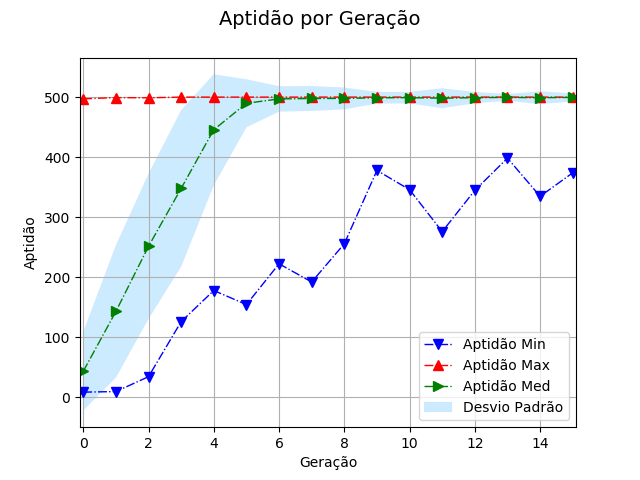
\includegraphics[width=0.8\textwidth]{02_desenvolvimento/04_EC_Fig_CartpoleAptGer.png}
	\caption{Média da aptidão de todos os indivíduos por geração (verde). Valor máximo de aptidão observado em cada geração (vermelho). Menor aptidão observada em cada geração (azul).}
	\label{fig:4ec-cartpoleaptger}
\end{figure}

Observa-se no gráfico da Figura \ref{fig:4ec-cartpoleaptger}, que na primeira geração alguns indivíduos já são capazes de obter a aptidão máxima. Isto se deve, em parte, ao grande número de indivíduos (500) gerados aleatoriamente, o que funciona, de certa forma, como uma busca exaustiva.

Entretanto, ainda é possível observar o aumento da aptidão média e mínima ao longo das gerações. O gráfico da Figura \ref{fig:4ec-cartpoleapthist} mostra o número de indivíduos que atingiram uma determinada faixa de aptidão, em algumas geração.

\begin{figure}[H]
	\centering
	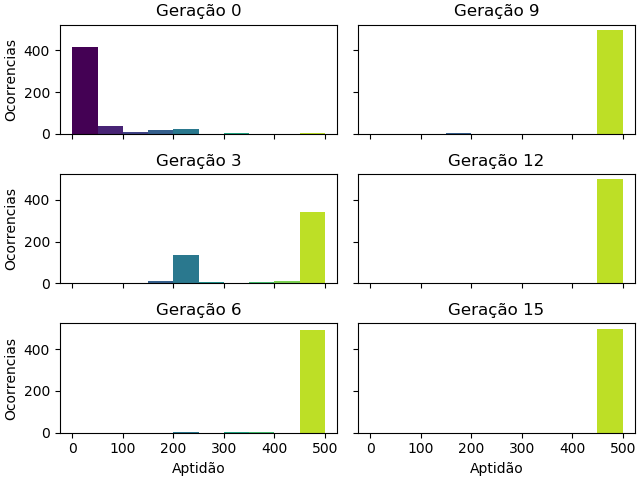
\includegraphics[width=0.8\textwidth]{02_desenvolvimento/04_EC_Fig_CartpoleAptHist.png}
	\caption{Número de indivíduos, em algumas gerações, que obtiveram cada faixa de aptidão.}
	\label{fig:4ec-cartpoleapthist}
\end{figure}

Conforme visto no Capítulo \ref{ssec:3deap-opgeneticos}, existe uma tendência de aumento do comprimento dos indivíduos ao longo do processo. O gráfico da Figura \ref{fig:4ec-cartpolecompr} mostra a média do comprimento de cada indivíduo em cada geração, assim como os valores mínimos e máximos observados. Já que todas as estatísticas foram obtidas através do valor médio em 10 execuções do algoritmo, o gráfico contém valores fracionários.

\begin{figure}[H]
	\centering
	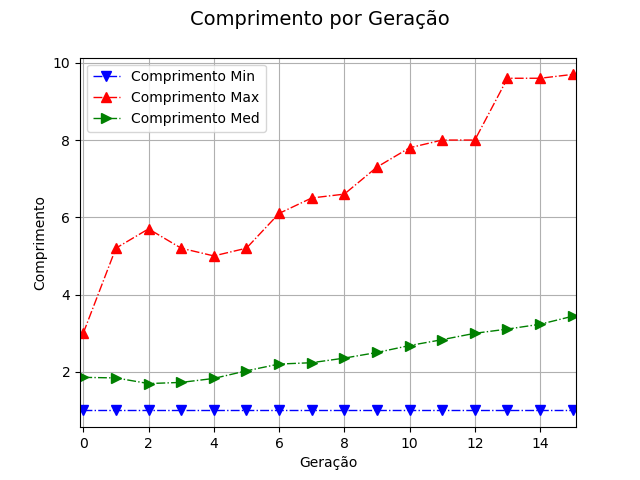
\includegraphics[width=0.8\textwidth]{02_desenvolvimento/04_EC_Fig_CartpoleCompr.png}
	\caption{Comprimento dos indivíduos por geração.}
	\label{fig:4ec-cartpolecompr}
\end{figure}

A complexidade dos indivíduos ao longo do processo pode ser observada no gráfico da Figura \ref{fig:4ec-cartpolecompl}.

\begin{figure}[H]
	\centering
	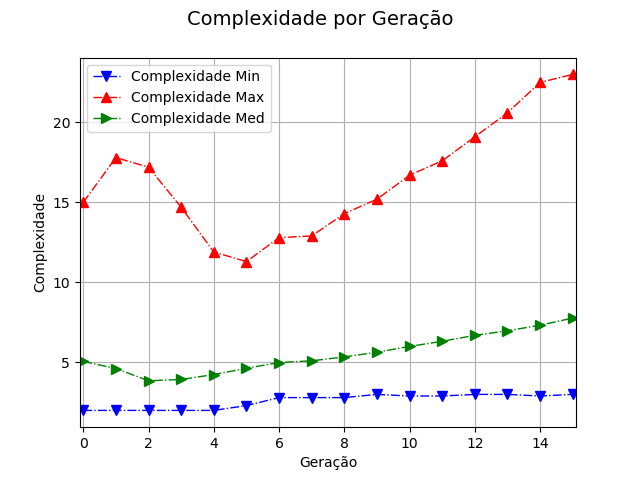
\includegraphics[width=0.8\textwidth]{02_desenvolvimento/04_EC_Fig_CartpoleCompl.png}
	\caption{Complexidade dos indivíduos em cada geração. }
	\label{fig:4ec-cartpolecompl}
\end{figure}

Foi possível observar que, alguns operadores e variáveis, pertencentes ao conjunto primitivo, são mais eficientes para a resolução do problema e tendem a aparecer com maior frequência à medida que a população se torna mais apta. Foi realizada a contagem dos operadores e variáveis de cada indivíduo pertencente à geração final, o resultado pode ser verificado no gráfico da Figura \ref{fig:4ec-cartpoleoper}.

\begin{figure}[H]
	\centering
	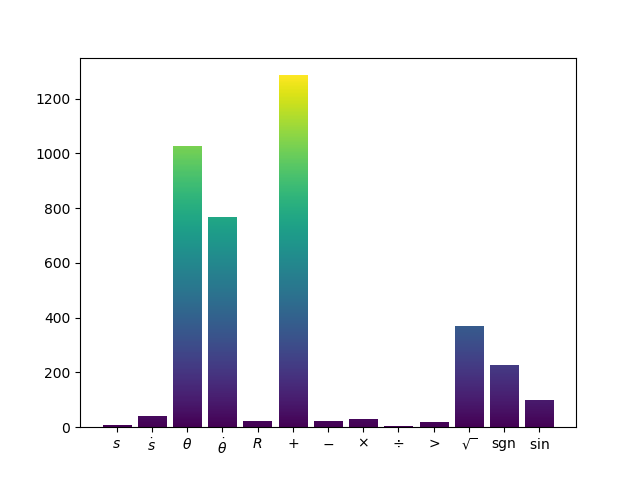
\includegraphics[width=0.8\textwidth]{02_desenvolvimento/04_EC_Fig_CartpoleOper.png}
	\caption{Número de ocorrências dos operadores e variáveis terminais, nos indivíduos da última geração.}
	\label{fig:4ec-cartpoleoper}
\end{figure}

Através do objeto \textit{hall da fama}, foi possível armazenar os indivíduos mais aptos que existiram na população ao longo de todo o processo de evolução. Esse objeto é atualizado a cada geração, de modo que o primeiro indivíduo possui a maior aptidão encontrada durante toda a execução do algoritmo evolucionário. Além disso, por ser um objeto de tamanho fixo, os indivíduos de gerações mais antigas possuem prioridade.

Na Figura \ref{fig:4ec-cartpoleindiv1}, é possível ver o primeiro indivíduo do hall da fama. Já que na geração inicial alguns indivíduos obtiveram a aptidão máxima, a solução da Figura \ref{fig:4ec-cartpoleindiv1} tem prioridade sobre as outras. O pequeno comprimento do indivíduo indica que, de fato, pertence às primeiras gerações.

\begin{figure}[H]
	\centering
	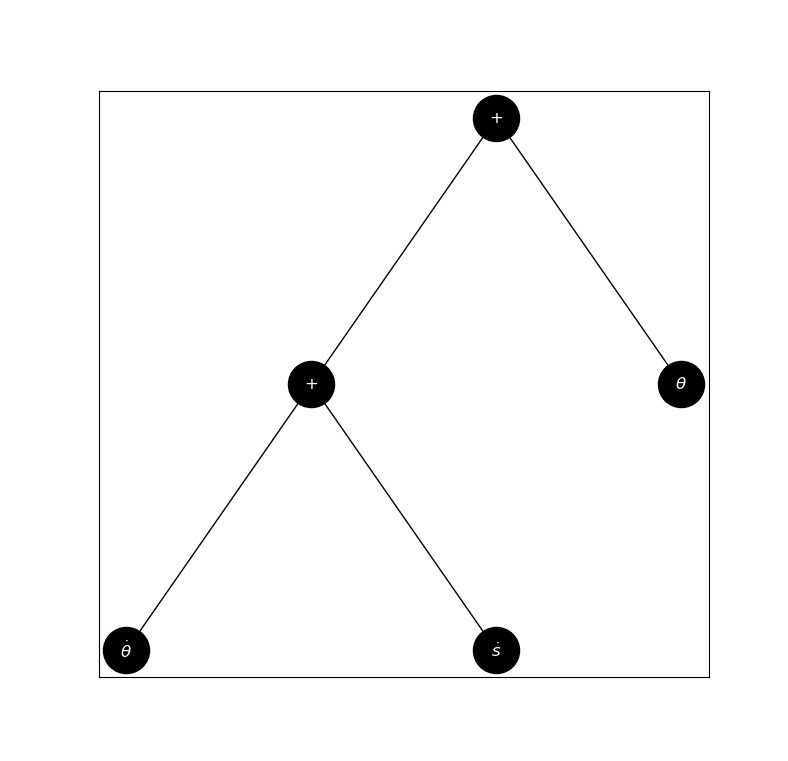
\includegraphics[width=\textwidth]{02_desenvolvimento/04_EC_Fig_CartpoleIndiv1.png}
	\caption{Primeiro indivíduo do hall da fama, na primeira execução do algoritmo.}
	\label{fig:4ec-cartpoleindiv1}
\end{figure}

É possível perceber indivíduos de maior comprimento, nas posições finais do hall da fama, como, por exemplo, na Figura \ref{fig:4ec-cartpoleindiv2}.

\begin{figure}[H]
	\centering
	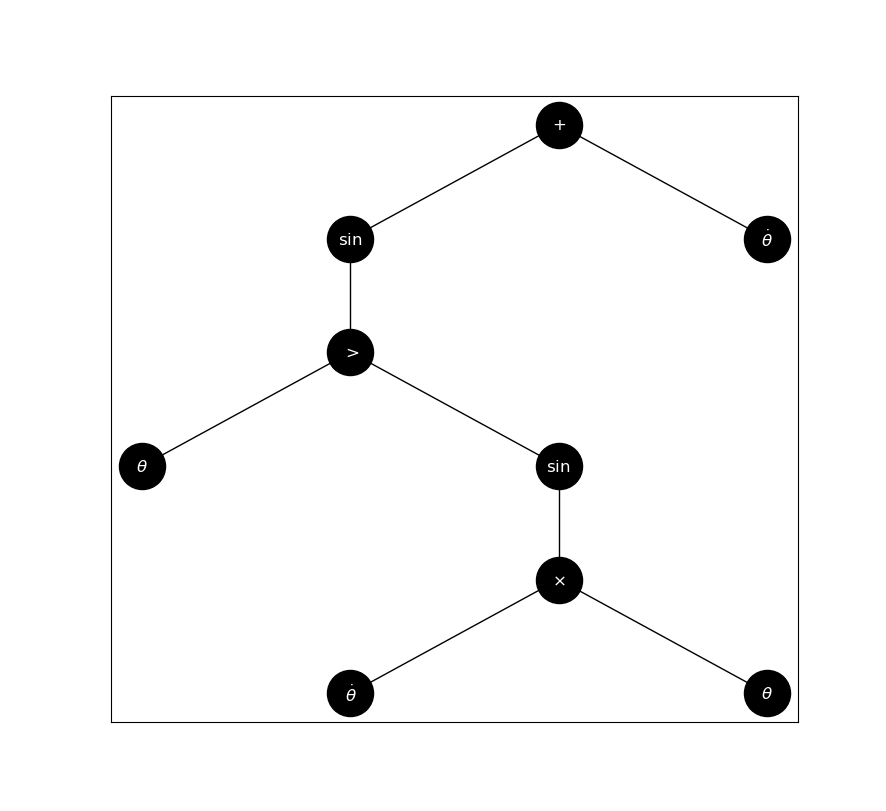
\includegraphics[width=\textwidth]{02_desenvolvimento/04_EC_Fig_CartpoleIndiv2.png}
	\caption{Vigésimo terceiro indivíduo do hall da fama, na primeira execução do algoritmo.}
	\label{fig:4ec-cartpoleindiv2}
\end{figure}

Já que múltiplos indivíduos obtiveram um bom desempenho em cada geração, incluindo as iniciais, é interessante notar o comprimento desses indivíduos mais aptos, especificamente. Pode-se observar que a tendência de aumento do comprimento dos indivíduos ao longo das gerações é preservada.

\begin{figure}[H]
	\centering
	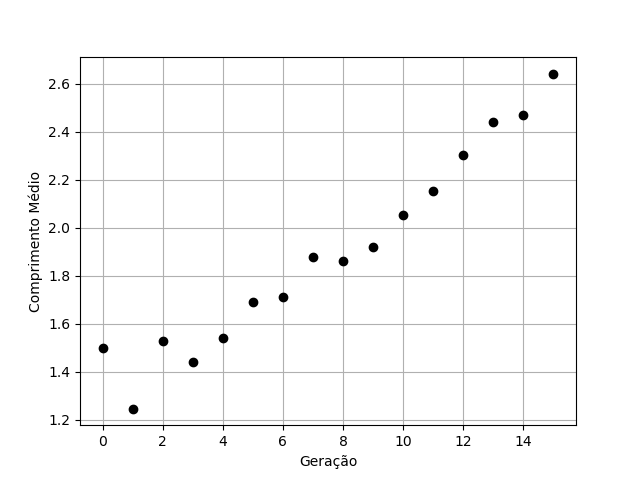
\includegraphics[width=0.7\textwidth]{02_desenvolvimento/compr_medio.png}
	\caption{Comprimento médio dos indivíduos que obtiveram aptidão maior que 400.}
	\label{fig:4ec-cartpolegrafaval}
\end{figure}

A Figura \ref{fig:4ec-cartpolegrafaval} mostra os gráficos relacionados à atuação do indivíduo da Figura \ref{fig:4ec-cartpoleindiv1}, em um único episódio. O eixo \textit{ação} indica o controle aplicado no sistema, a partir do \textit{resultado} obtido no cálculo da expressão matemática que representa um indivíduo.

\begin{figure}[H]
	\centering
	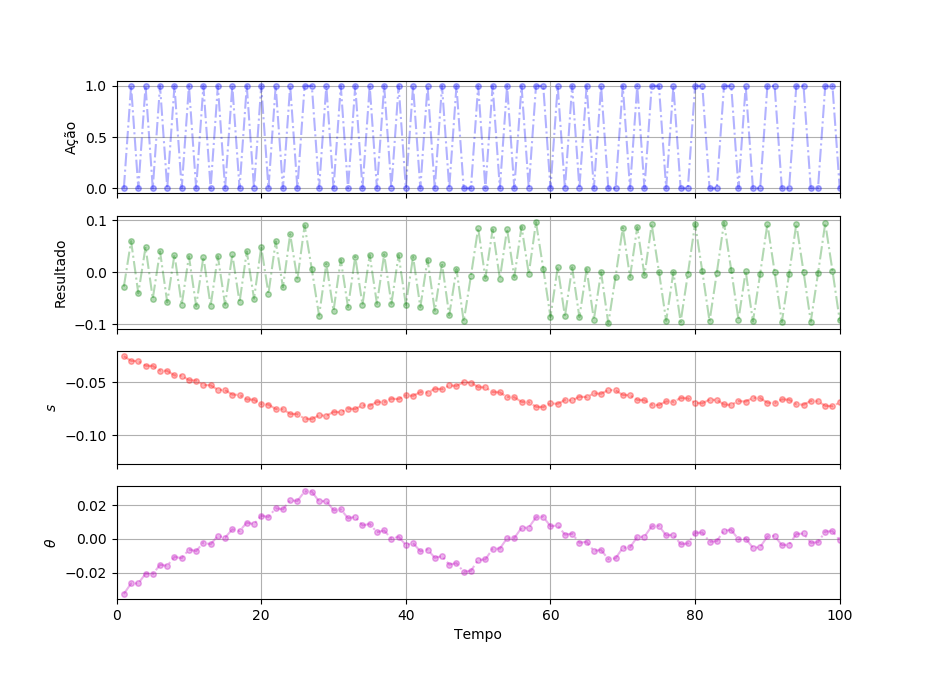
\includegraphics[width=\textwidth]{02_desenvolvimento/04_EC_Fig_CartpoleGraficosAval.png}
	\caption{Controle do sistema pelo indivíduo da Figura \ref{fig:4ec-cartpoleindiv1}. O pêndulo é levado rapidamente a um estado de baixa oscilação.}
	\label{fig:4ec-cartpolegrafaval}
\end{figure}

Foi possível observar que os indivíduos aptos pertencentes ao hall da fama são capazes de manter um valor baixo de oscilação do ângulo, ao redor do zero, entretanto, algumas soluções causavam a posição do carrinho a tender para um dos extremos, o que levava ao término antecipado do episódio.

Já que as aptidões dos indivíduos foram estimadas a partir de 10 simulações, é possível que as melhores soluções tenham sido beneficiadas por condições iniciais vantajosas. Não é possível, entretanto, aumentar o número de simulações sem que haja um aumento considerável no tempo de execução do algoritmo.

Dessa forma, é interessante verificar a aptidão dos indivíduos do hall da fama, em um grande número de episódios. Portanto, busca-se o indivíduo mais apto ao avaliar cada membro do hall da fama em 100 simulações.

A situação inicial do ambiente é determinada de forma aleatória, dentro de uma faixa específica característica de cada problema na biblioteca Gym. As condições iniciais de cada ambiente podem ser observadas no apêndice \ref{apendice:cond-iniciais}.

É proveitoso realizar a comparação desses resultados com a abordagem proposta pelo algoritmo DQN, uma vez que o critério de desempenho é o mesmo, isto é, a média de recompensa acumulada em vários episódios. O tempo médio de execução do algoritmo de PG foi \SI{334}{s}. O agente DQN é treinado, aproximadamente, pelo mesmo tempo. Em seguida, as recompensas médias acumuladas por episódio, em 100 simulações são comparadas. Destaca-se que a avaliação da PG foi realizada pelo indivíduo mais apto do hall da fama, quando cada membro é submetido à 100 episódios.

Utilizando a biblioteca \textit{stable-baselines} \cite{stable-baselines}, o agente DQN foi treinado por \SI{334}{s} (código encontra-se no apêndice). O gráfico da Figura \ref{fig:4ec-cartpoledqndiverg} mostra a recompensa obtida pelo agente ao longo do treinamento.

\begin{figure}[H]
	\centering
	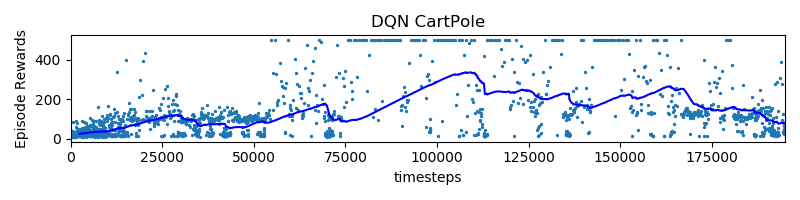
\includegraphics[width=0.85\textwidth]{02_desenvolvimento/04_EC_Fig_CartpoleDQNDiverg.png}
	\caption{Recompensa média acumulada em função do número de passos de simulação. A linha contínua representa a média móvel.}
	\label{fig:4ec-cartpoledqndiverg}
\end{figure}

Na Figura \ref{fig:4ec-cartpoledqndiverg} é possível notar a degradação da recompensa média acumulada a partir dos 110000 passos de simulação. Já que esse comportamento foi observado, o algoritmo foi executado novamente com o número de passos totais reduzido. O resultado pode ser verificado na Figura \ref{fig:4ec-cartpoledqngraf}.

\begin{figure}[H]
	\centering
	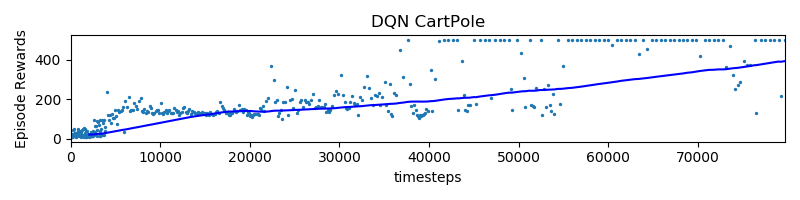
\includegraphics[width=0.85\textwidth]{02_desenvolvimento/04_EC_Fig_CartpoleDQNGraf.png}
	\caption{Recompensa média ao longo dos passos de simulação. A linha azul contínua indica a média móvel.}
	\label{fig:4ec-cartpoledqngraf}
\end{figure}

A Tabela \ref{tab:4ec-cartpolecomp} sumariza uma breve comparação entre o desempenho da programação genética com o algoritmo DQN, em termos de custos computacionais.

\begin{table}[H]
	\centering
	\begin{tabular}{SSS} \toprule
		{} & {{PG}} & {{DQN}} \\ \midrule
		{{Desempenho}} & {497} & {500} \\
		{{Tempo de execução (s)}} & {334} & {280} \\
		{{Passos de simulação}} & {16647338} & {80000} \\
		{{Número de episódios}} & {65095} & {450\footnotemark} \\
		\bottomrule
	\end{tabular}
	\caption{Comparação entre a programação genética e DQN, para o problema do pêndulo invertido.}\label{tab:4ec-cartpolecomp}
\end{table}

\footnotetext[1]{Valor estimado.}

A Figura \ref{fig:4ec-cartpoledqnvargraf} mostra a atuação do agente DQN, ao longo de um episódio.

\begin{figure}[H]
	\centering
	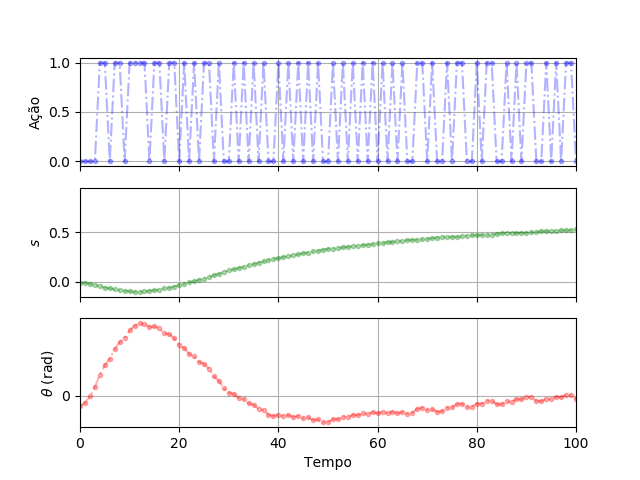
\includegraphics[width=0.85\textwidth]{02_desenvolvimento/04_EC_Fig_CartpoleDQNVarGraf.png}
	\caption{Posição do carrinho e ângulo do bastão, em função do tempo, com a atuação do agente DQN.}
	\label{fig:4ec-cartpoledqnvargraf}
\end{figure}

Observa-se, por fim, que as duas abordagens foram capazes de encontrar soluções satisfatórias para o problema. A seguir, serão abordados outros problemas que envolvem pêndulos e sua estabilização.

\subsection{Pêndulo \textit{Swing-up}}\label{ssec:4ec-pendulum}

O próximo sistema abordado está disponível na biblioteca Gym, na seção \textit{classic control}, direcionada à implementação de ambientes de simulações para problemas clássicos de controle. Conforme a abordagem do problema anterior, são introduzidos os critérios de término do episódio, as variáveis de estado observáveis e a implementação da recompensa. A formulação da função de aptidão, a partir da recompensa disponível, também é abordada.

A dinâmica envolve um bastão com uma de suas extremidades fixas, sendo possível a atuação do agente a partir da aplicação de um torque, em qualquer sentido, buscando a manutenção da extremidade livre na posição mais alta. A Figura \ref{fig:4ec-pendulumenv} ilustra o problema.

\begin{figure}[H]
	\centering
	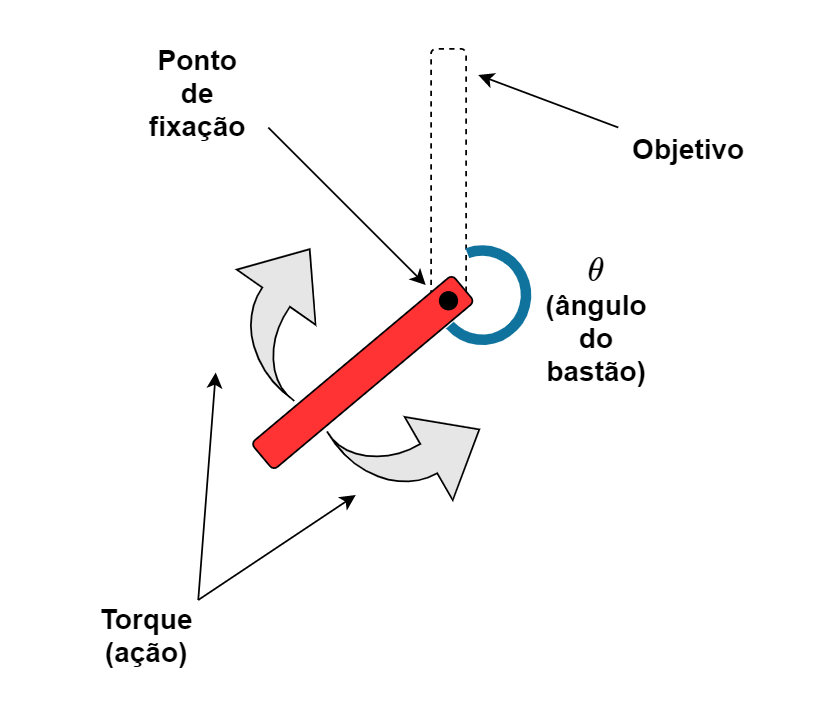
\includegraphics[width=0.7\textwidth]{02_desenvolvimento/04_EC_Fig_PendulumEnv2.png}
	\caption{Pêndulo \textit{Swing-up}.}
	\label{fig:4ec-pendulumenv}
\end{figure}

A seguir são enumerados alguns aspectos que aumentam a complexidade do problema, além de outras diferenças fundamentais do ambiente, em comparação com o pêndulo invertido:

\begin{itemize}[label=\raisebox{0.25ex}{\tiny$\bullet$}]
	\item O ponto de equilíbrio é estável.
	\item O torque aplicado em um único sentido, a partir da posição de repouso, não permite alcançar o objetivo em um movimento contínuo (o bastão precisa adquirir momento para superar a força gravitacional).
	\item As ações possíveis se dão no espaço contínuo.
	\item As recompensas são implementadas a partir de uma função custo.
\end{itemize}

A Tabela \ref{tab:4ec-pendulumvarestado} apresenta as variáveis que indicam o estado do sistema e que são fornecidas como uma \textit{observação}, após cada ação do agente. Já que o ponto de equilíbrio do sistema é estável, o único critério de término é o tempo de simulação. Com base na documentação da biblioteca Gym \cite{openaigym}, isto ocorre após 200 passos de simulação.

\begin{table}[H]
	\centering
	\caption{Variáveis que compõem a observação do pêndulo swing-up.}
	\label{tab:4ec-pendulumvarestado}
	\begin{tabular}{l|l} \toprule
		{Variável} & {Significado}\\ \midrule
		{$\cos(\theta)$} & {Cosseno do ângulo do bastão} \\
		{$\sin(\theta)$} & {Seno do ângulo do bastão} \\
		{$\dot{\theta}$} & {Velocidade angular do bastão} \\
		\bottomrule
	\end{tabular}
\end{table}

Seguindo a abordagem do Capítulo \ref{ssec:3deap-avalind}, é criada uma função de aptidão para o indivíduo. A recompensa a cada instante de tempo é uma função custo, segundo a Equação \ref{eq:4ec-pendulumrewardfunction}.

\begin{align}\label{eq:4ec-pendulumrewardfunction}
\begin{split}
r(t) = - \left[(\theta(t))^2 + 0,1(\dot\theta(t))^2+0,001(a(t))^2\right]\qquad &-\pi \le \theta \le \pi\\\\
&-2 \le a(t) \le 2
\end{split}
\end{align}

A variável $a(t)$ representa a ação (torque) do agente, no instante de tempo $t$. Foi mencionado no Capítulo \ref{sec:1pg-apg} a possibilidade de projetar a função de aptidão utilizando uma penalização por desvios de um estado de referência. Desta forma, o desempenho de um indivíduo é dado pela soma dos custos (implementados como recompensas negativas) em vários episódios:

\begin{align}\label{eq:4ec-pendulumaptidao}
\begin{split}
A(t) &= r(t) = - \left[\left[\theta(t)\right]^2 + 0,1\left[\dot\theta(t)\right]^2+0,001\left[a(t)\right]^2\right]\\\\
A_{tot}^{ep} &= \sum_{t=0}^{T} A(t) = - \sum_{t=0}^{T} \left[
\left[\theta(t)\right]^2 + 0,1\left[\dot\theta(t)\right]^2+0,001\left[a(t)\right]^2
\right]\qquad T \le 200\\\\
\bar{A} &= \dfrac{1}{nep}\sum_{ep=1}^{nep} A_{tot}^{ep} =
-\dfrac{1}{nep}\sum_{ep=1}^{nep}\sum_{t=0}^{T} \left[
\left[\theta(t)\right]^2 + 0,1\left[\dot\theta(t)\right]^2+0,001\left[a(t)\right]^2
\right]
\end{split}
\end{align}

De forma maneira similar ao problema anterior, o objetivo é \underline{maximizar} a aptidão média na Equação \ref{eq:4ec-pendulumaptidao}.

Buscando demonstrar a robustez da PG, poucas mudanças foram realizadas nos parâmetros da Tabela \ref{tab:4ec-param-cartpole}, mais especificamente, foram alterados: o número de entradas, comprimentos de inicialização e o comprimento máximo de mutação.

\begin{table}[H]
	\centering
	\begin{tabular}{l|l} \toprule
		{Parâmetro} & {Valor} \\ \midrule
		{Tamanho da População} & {500} \\
		{Probabilidade de Cruzamento} & {0,75} \\
		{Probabilidade de Mutação} & {0,05} \\
		{Número de Gerações} & {15} \\
		{Número de Entradas} & {3} \\
		{Faixa para Constante Efêmera} & {(-1, 1)} \\
		{Número de Simulações} & {10} \\
		{Tamanho do Campeonato de Aptidão} & {6} \\
		{Tamanho do Campeonato de Comprimento} & {1,2} \\
		{Operações} & {$+,\,-,\,\times,\,\div,\,\sqrt{},\,\sin,\,>$, sgn} \\
		{Comprimento Mínimo e Máximo de Inicialização} & {(2, 5)} \\
		{Comprimento Máximo de Mutação} & {7} \\
		{Limite de Comprimento dos Indivíduos} & {17} \\
		\bottomrule
	\end{tabular}
	\caption{Parâmetros da programação genética aplicada ao pêndulo swing-up.}\label{tab:4ec-pendulumparam}
\end{table}

É interessante destacar que o problema do Capítulo \ref{ssec:4ec-cartpole} utilizava ações discretas. Logo, bastava mapear os valores que resultavam da compilação das árvores em ações: números positivos produziam uma força para a direita no carrinho, enquanto os negativos geravam uma ação no sentido contrário.

Neste problema, o espaço de ações é contínuo, portanto é necessário apenas garantir que o resultado matemático da compilação de um indivíduo obedeça aos limites de torque, definidos na Equação \ref{eq:4ec-pendulumrewardfunction}. Isto pode ser concebido pela utilização da função \textit{clip}, cujo comportamento é demonstrado na Figura \ref{fig:4ec-pendulumclip}.

\begin{figure}[H]
	\centering
	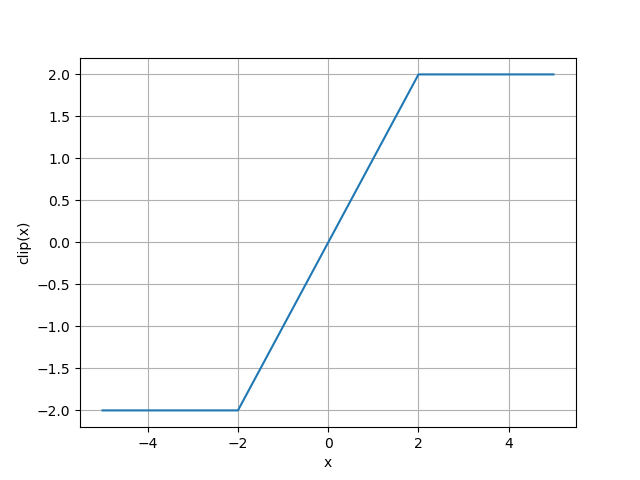
\includegraphics[width=0.82\textwidth]{02_desenvolvimento/04_EC_Fig_PendulumClipFun.png}
	\caption{Função \textit{clip}.}
	\label{fig:4ec-pendulumclip}
\end{figure}

Essa função funcionará como \textit{wrapper}, isto é, um mapeamento de um valor numérico em uma ação admissível.

Novamente, o algoritmo foi executado 10 vezes e a média das estatísticas foram obtidas. A começar pela aptidão ao longo das gerações, onde é possível perceber que a busca inicial da primeira geração, através da inicialização, não pôde obter um resultado satisfatório, como no problema anterior. As próximas gerações encontram uma solução eficaz para o pêndulo, conforme pode ser visto nas Figuras \ref{fig:4ec-pendulumaptger} e \ref{fig:4ec-pendulumapthist}.

\begin{figure}[H]
	\centering
	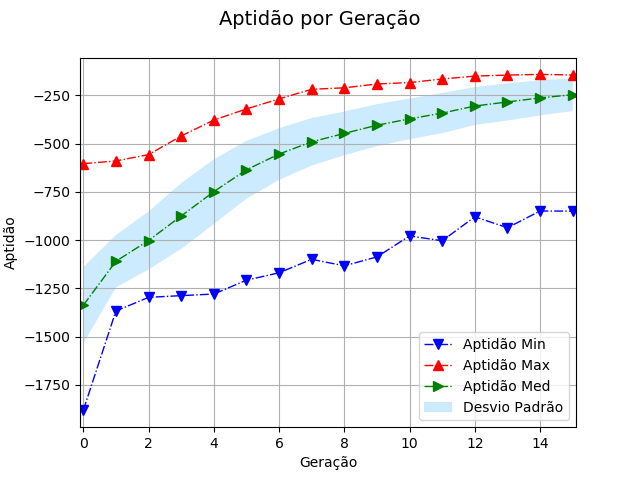
\includegraphics[width=0.85\textwidth]{02_desenvolvimento/04_EC_Fig_PendulumAptGer.png}
	\caption{Aptidão dos indivíduos, ao longo das gerações.}
	\label{fig:4ec-pendulumaptger}
\end{figure}

\begin{figure}[H]
	\centering
	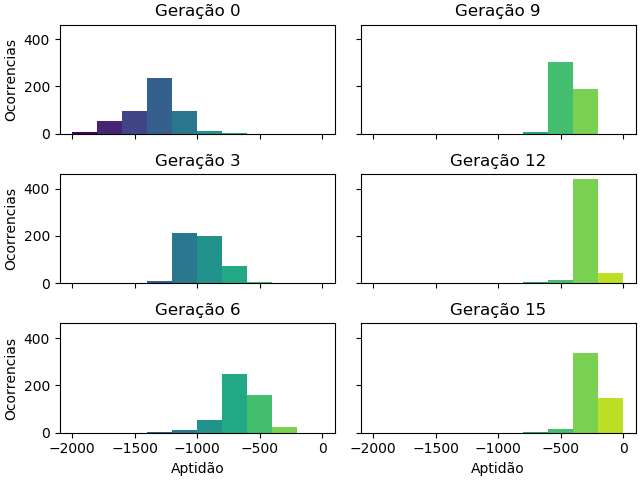
\includegraphics[width=0.85\textwidth]{02_desenvolvimento/04_EC_Fig_PendulumAptHist.png}
	\caption{Histograma da aptidão dos indivíduos.}
	\label{fig:4ec-pendulumapthist}
\end{figure}

O comprimento e a complexidade dos indivíduos da população, ao longo das gerações, podem ser vistos nas Figuras \ref{fig:4ec-pendulumcompr} e \ref{fig:4ec-pendulumcompl}, respectivamente.

\begin{figure}[H]
	\centering
	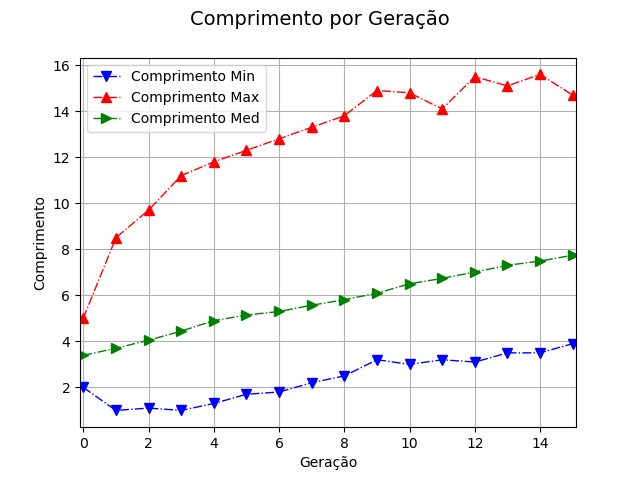
\includegraphics[width=0.85\textwidth]{02_desenvolvimento/04_EC_Fig_PendulumCompr.png}
	\caption{Comprimento dos indivíduos.}
	\label{fig:4ec-pendulumcompr}
\end{figure}

\begin{figure}[H]
	\centering
	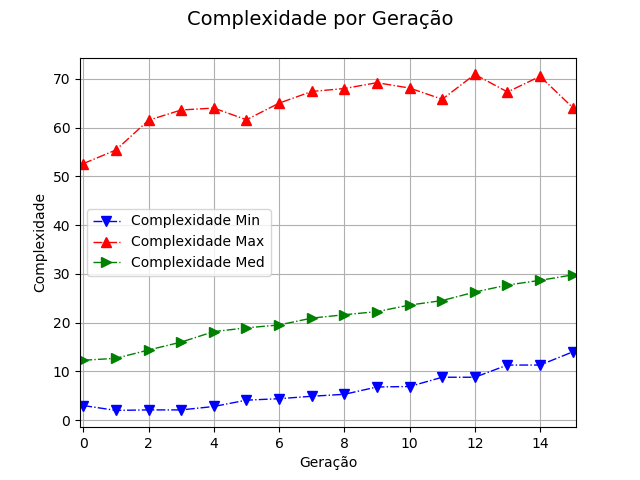
\includegraphics[width=0.85\textwidth]{02_desenvolvimento/04_EC_Fig_PendulumCompl.png}
	\caption{Complexidade dos indivíduos.}
	\label{fig:4ec-pendulumcompl}
\end{figure}

A Figura \ref{fig:4ec-pendulumoper} mostra o número de ocorrências dos operadores e variáveis terminais, na população da última geração.

\begin{figure}[H]
	\centering
	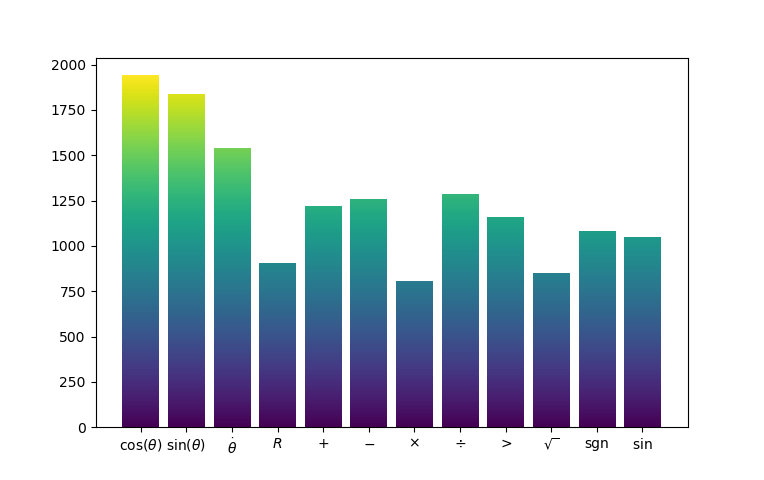
\includegraphics[width=0.85\textwidth]{02_desenvolvimento/04_EC_Fig_PendulumOper.png}
	\caption{Histograma de operadores e variáveis terminais, na última geração.}
	\label{fig:4ec-pendulumoper}
\end{figure}

O indivíduo de maior aptidão, na primeira execução, é mostrado na Figura \ref{fig:4ec-pendulumindiv1}.

\begin{figure}[H]
	\centering
	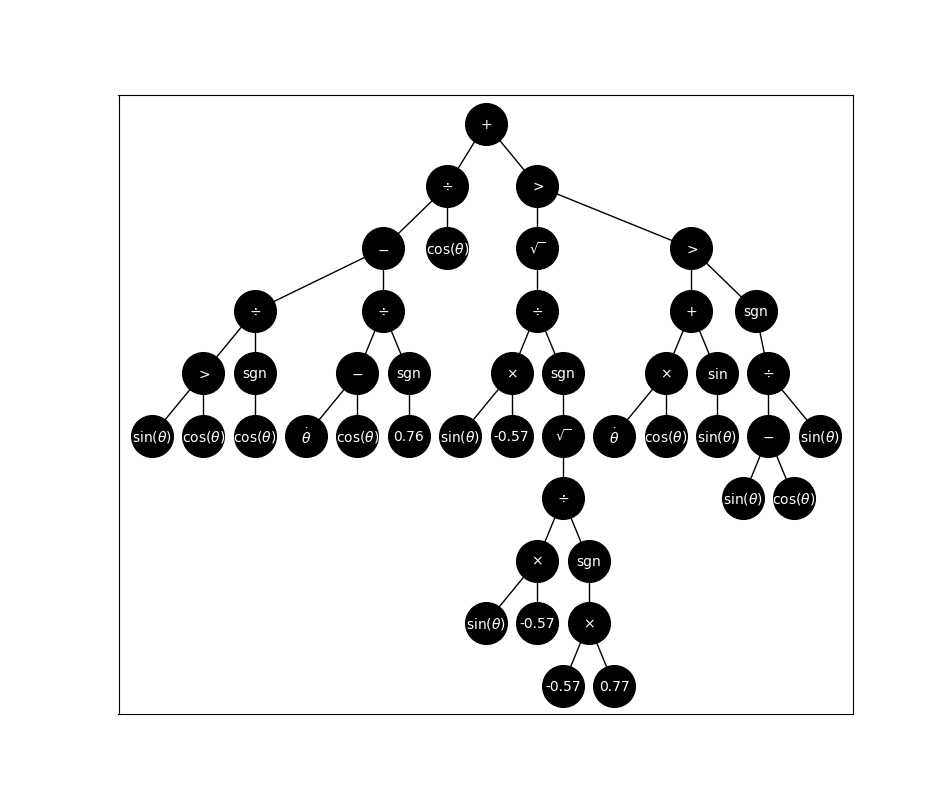
\includegraphics[width=\textwidth]{02_desenvolvimento/04_EC_Fig_PendulumIndiv1.png}
	\caption{Primeiro integrante do hall da fama.}
	\label{fig:4ec-pendulumindiv1}
\end{figure}

O segundo integrante do hall da fama, na primeira execução, é mostrado na Figura \ref{fig:4ec-pendulumindiv2}.

\begin{figure}[H]
	\centering
	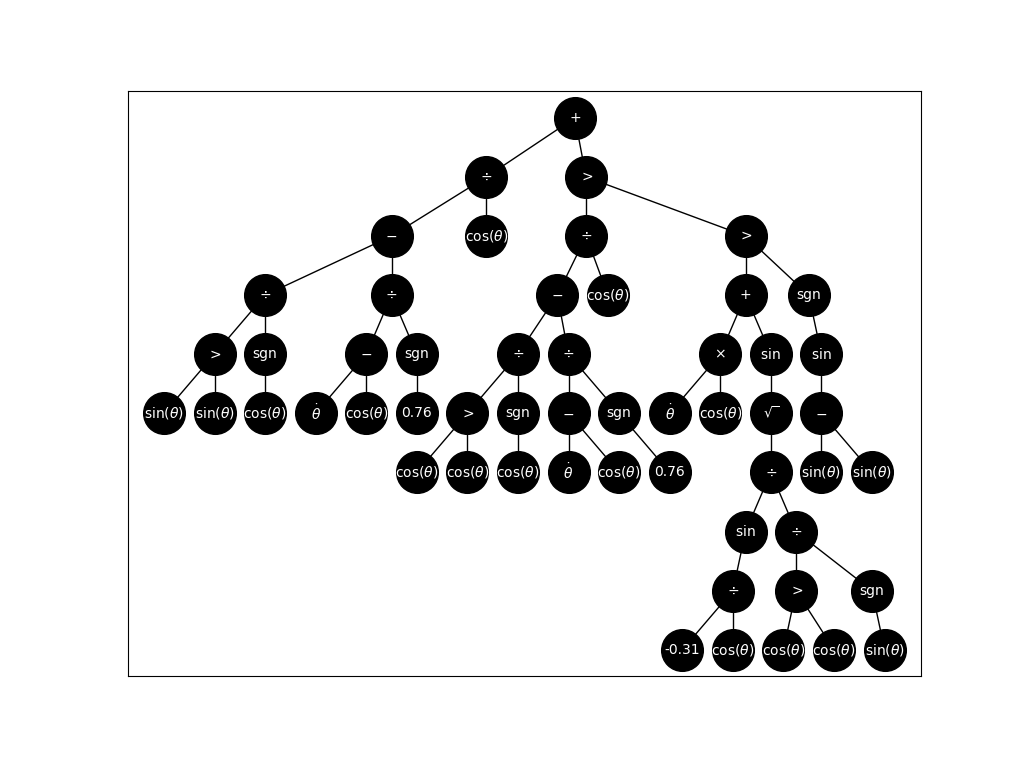
\includegraphics[width=\textwidth]{02_desenvolvimento/04_EC_Fig_PendulumIndiv2.png}
	\caption{Segundo integrante do hall da fama.}
	\label{fig:4ec-pendulumindiv2}
\end{figure}

A Figura \ref{fig:4ec-pendulumgraficosaval} mostra as ações, o ângulo e velocidade angular do bastão, quando o sistema é submetido ao controle do indivíduo da Figura \ref{fig:4ec-pendulumindiv1}, em um único episódio.

\begin{figure}[H]
	\centering
	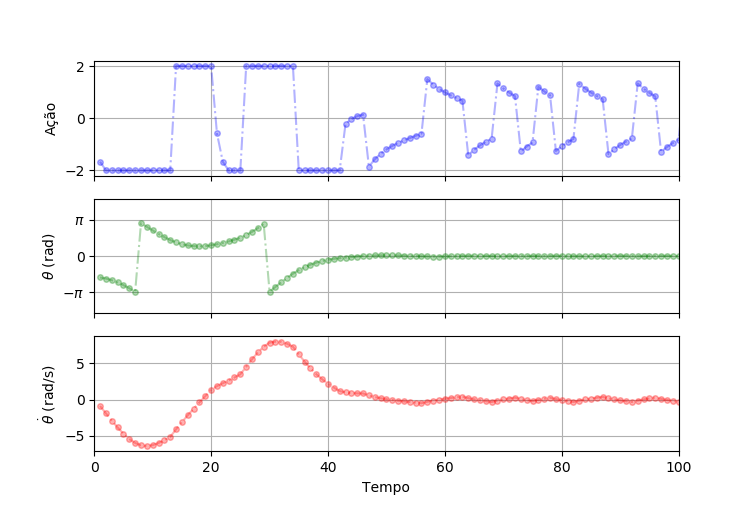
\includegraphics[width=0.95\textwidth]{02_desenvolvimento/04_EC_Fig_PendulumGraficosAval.png}
	\caption{Controle exercido pelo indivíduo da Figura \ref{fig:4ec-pendulumindiv1}.}
	\label{fig:4ec-pendulumgraficosaval}
\end{figure}

As transições bruscas no ângulo $\theta$ indicam a passagem da extremidade livre do pêndulo no ponto mais baixo, onde a função adquiri o maior valor absoluto. Após alguns instantes, o ângulo do bastão oscila em torno do zero de forma estável.

Utilizando a mesma metodologia do Capítulo \ref{ssec:4ec-cartpole}, é feita a avaliação em 100 episódios dos indivíduos do hall da fama. O maior valor de aptidão obtido é comparado com a recompensa acumulada de um agente treinado com o algoritmo DDPG, que pode ser visto como uma extensão do algoritmo DQN para ambientes com ações no espaço contínuo. Novamente, a medida de desempenho de um agente é obtida através função de recompensa disponibilizada pelo ambiente de simulação. Com isso, é possível realizar uma comparação direta entre as duas abordagens.

A Figura \ref{fig:4ec-pendulumddpggraf} mostra o agente DDPG sendo treinado em 100000 passos de tempo.

\begin{figure}[H]
	\centering
	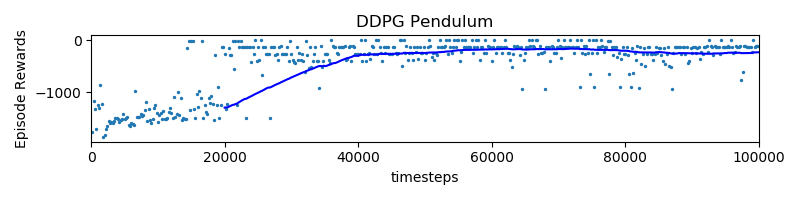
\includegraphics[width=0.9\textwidth]{02_desenvolvimento/04_EC_Fig_PendulumDDPGGraf.png}
	\caption{Evolução da recompensa acumulada para o agente DDPG no pêndulo swing-up.}
	\label{fig:4ec-pendulumddpggraf}
\end{figure}

A atuação do agente em um episódio pode ser vista na Figura \ref{fig:4ec-pendulumddpgvargraf}.

\begin{figure}[H]
	\centering
	\includegraphics[width=0.9\textwidth]{02_desenvolvimento/04_EC_Fig_PendulumDDPGVarGraf.png}
	\caption{Dinâmica do pêndulo swing-up sob ação do agente DDPG.}
	\label{fig:4ec-pendulumddpgvargraf}
\end{figure}

\begin{table}[H]
	\centering
	\begin{tabular}{l|l|l} \toprule
		{} & {PG} & {{DDPG}} \\ \midrule
		{Desempenho} & {-230} & {-253} \\
		{Tempo de execução (s)} & {1649} & {194} \\
		{Passos de simulação} & {13034400} & {100000} \\
		{Número de episódios} & {65172} & {500} \\
		\bottomrule
	\end{tabular}
	\caption{Comparação entre a programação genética e DDPG para o pêndulo swing-up.}\label{tab:4ec-pendulumcomp}
\end{table}

É possível notar a partir da Tabela \ref{tab:4ec-pendulumcomp} que as duas abordagens são capazes de resolver o problema de controle proposto.

\subsection{Pêndulo Duplo Invertido}\label{ssec:4ec-dp}

Este problema é similar ao pêndulo invertido, pois a estabilização do bastão envolve a movimentação do veículo (que contém o ponto de fixação) sobre uma trilha. A diferença reside na existência de um outro bastão, fixado na extremidade antes livre, aumentando consideravelmente a complexidade do problema. As Figuras \ref{fig:4ec-dpenv} e \ref{fig:4ec-dpenv2} mostram o sistema proposto.

\begin{figure}[H]
	\centering
	\includegraphics[width=0.8\textwidth]{02_desenvolvimento/04_EC_Fig_DPEnv.png}
	\caption{Renderização 3D do sistema pêndulo duplo invertido.}
	\label{fig:4ec-dpenv}
\end{figure}

\begin{figure}[H]
	\centering
	\includegraphics[width=0.8\textwidth]{02_desenvolvimento/04_EC_Fig_DPEnv2.png}
	\caption{Ângulos $\theta$, $\gamma$ e a posição do veículo ($s$).}
	\label{fig:4ec-dpenv2}
\end{figure}

A observação do sistema é composta de 11 variáveis:

\begin{table}[H]
	\centering
	\caption{Variáveis disponibilizadas como observação do pêndulo duplo invertido.}
	\label{tab:4ec-dpvarestado}
	\begin{tabular}{l|l} \toprule
		{Variável} & {Significado}\\ \midrule
		{$s$} & {Posição do carrinho} \\
		{$\sin(\theta)$} & {Seno do ângulo do bastão inferior} \\
		{$\sin{(\gamma)}$} & {Seno do ângulo do bastão superior} \\
		{$\cos(\theta)$} & {Cosseno do ângulo do bastão inferior} \\
		{$\cos(\gamma)$} & {Cosseno do ângulo do bastão superior} \\
		{$\dot{s}$} & {Velocidade do carrinho} \\
		{$\dot{\theta}$} & {Velocidade angular do bastão inferior} \\
		{$\dot{\gamma}$} & {Velocidade angular do bastão superior} \\
		{$f_r(s)$} & {Força de restrição em função da posição} \\
		{$f_r(\theta)$} & {Força de restrição em função de $\theta$} \\
		{$f_r(\gamma)$} & {Força de restrição em função de $\gamma$} \\
		\bottomrule
	\end{tabular}
\end{table}

Conforme a abordagem realizada até o momento, todas as variáveis da Tabela \ref{tab:4ec-dpvarestado} fazem parte do conjunto primitivo. Os outros parâmetros foram mantidos iguais ao do problema anterior (Tabela \ref{tab:4ec-pendulumparam}).

A função de recompensa do ambiente de simulação, a cada instante de tempo, pode ser vista na Equação \ref{eq:4ec-dprewardfunction}.

\begin{align}\label{eq:4ec-dprewardfunction}
\begin{split}
r(t) &= 10 - d_p(t) - v_p(t)\\\\
d_p(t) &= 0,01\left[s(t)\right]^2 + \left[y(t)-2\right]^2\\\\
v_p(t) &= 0,001\left[\dot{\theta}(t)\right]^2 + 0,005\left[\dot{\gamma}(t)\right]^2
\end{split}
\end{align}

Na Equação \ref{eq:4ec-dprewardfunction}, $d_p(t)$ e $v_p(t)$ são penalidades dadas em função da distância e das velocidades angulares dos bastões, respectivamente. A variável $y$ representa a altura da extremidade livre do bastão superior. Além de auxiliar no cálculo do custo, a quantidade $y$ também auxilia na verificação do término do episódio. Mais especificamente, a simulação encerra após 1000 passos de tempo ou quando a variável $y$ assume valores menores ou iguais a 1.

Naturalmente, a função de recompensa mostrada na Equação \ref{eq:4ec-dprewardfunction} será utilizada para o cálculo da aptidão de um indivíduo, utilizando a mesma formulação da Equação \ref{eq:4ec-pendulumaptidao}.

\begin{align}\label{eq:4ec-dpaptidao}
\begin{split}
A(t) &= r(t) = 10 - d_p(t) - v_p(t)\\\\
A_{tot}^{ep} &= \sum_{t=0}^{T} A(t) = - \sum_{t=0}^{T} \left[
10 - d_p(t) - v_p(t)
\right]\qquad T \le 1000\\\\
\bar{A} &= \dfrac{1}{nep}\sum_{ep=1}^{nep} A_{tot}^{ep} =
-\dfrac{1}{nep}\sum_{ep=1}^{nep}\sum_{t=0}^{T}
\left[
10 - d_p(t) - v_p(t)
\right]
\end{split}
\end{align}

Como o espaço de ações é contínuo, foi utilizada a função clip, da Figura \ref{fig:4ec-pendulumclip}, como wrapper para o resultado produzido pelas árvores. Entretanto, os valores extremos serão $-1$ e $1$, e não $-2$ e $2$.

As Figuras \ref{fig:4ec-dpapthist} a \ref{fig:4ec-dpcompl} mostram os resultados obtidos, através da média de 10 execuções do algoritmo.

\begin{figure}[H]
	\centering
	\includegraphics[width=0.8\textwidth]{02_desenvolvimento/04_EC_Fig_DPAptHist.png}
	\caption{Histograma da aptidão dos indivíduos, em algumas gerações, para o pêndulo duplo invertido.}
	\label{fig:4ec-dpapthist}
\end{figure}

\begin{figure}[H]
	\centering
	\includegraphics[width=0.8\textwidth]{02_desenvolvimento/04_EC_Fig_DPAptGer.png}
	\caption{Medidas de aptidão da população, em cada geração.}
	\label{fig:4ec-dpaptger}
\end{figure}

\begin{figure}[H]
	\centering
	\includegraphics[width=0.8\textwidth]{02_desenvolvimento/04_EC_Fig_DPCompr.png}
	\caption{Medidas de comprimento da população, ao longo das gerações.}
	\label{fig:4ec-dpcompr}
\end{figure}

\begin{figure}[H]
	\centering
	\includegraphics[width=0.8\textwidth]{02_desenvolvimento/04_EC_Fig_DPCompl.png}
	\caption{Medidas de complexidade dos indivíduos, em função das gerações.}
	\label{fig:4ec-dpcompl}
\end{figure}

\begin{figure}[H]
	\centering
	\includegraphics[width=\textwidth]{02_desenvolvimento/04_EC_Fig_DPOperHist.png}
	\caption{Número de ocorrências dos operadores e variáveis terminais, na última geração.}
	\label{fig:4ec-dpoperhist}
\end{figure}

Para cada indivíduo do hall da fama foram realizadas 100 simulações, com o intuito de verificar a solução mais apta e generalista. O indivíduo da Figura \ref{fig:4ec-dpindiv1} obteve uma aptidão média de 7794.

\begin{figure}[H]
	\centering
	\includegraphics[width=0.9\textwidth]{02_desenvolvimento/04_EC_Fig_DPIndiv1}
	\caption{Indivíduo mais apto da primeira execução do algoritmo.}
	\label{fig:4ec-dpindiv1}
\end{figure}

Os gráficos da Figura \ref{fig:4ec-dpvargraf} mostram os ângulos e a posição do carrinho, quando a solução da Figura \ref{fig:4ec-dpindiv1} atua em um episódio.

\begin{figure}[H]
	\centering
	\includegraphics[width=0.9\textwidth]{02_desenvolvimento/04_EC_Fig_DPVarGraf}
	\caption{Avaliação do melhor indivíduo observado na primeira execução.}
	\label{fig:4ec-dpvargraf}
\end{figure}

O gráfico da Figura \ref{fig:4ec-dpddpgtrain} mostra um agente sendo treinado com o algoritmo DDPG, por 400000 passos de simulação. A recompensa média acumulada pelo agente, em 100 episódios, pode ser vista na Tabela \ref{tab:4ec-dpcomp}, junto à outras estatísticas relacionadas ao custo computacional.

\begin{figure}[H]
	\centering
	\includegraphics[width=\textwidth]{02_desenvolvimento/04_EC_Fig_DPDDPGTrain}
	\caption{Evolução da recompensa acumulada do agente DDPG. A linha azul representa a média móvel.}
	\label{fig:4ec-dpddpgtrain}
\end{figure}

\begin{table}[H]
	\centering
	\begin{tabular}{l|l|l} \toprule
		{} & {{PG}} & {{DDPG}} \\ \midrule
		{{Desempenho}} & {7794} & {9019} \\
		{{Tempo de execução (s)}} & {2406} & {1230} \\
		{{Passos de simulação}} & {10392643} & {400000} \\
		{{Número de episódios}} & {64989} & {1230} \\
		\bottomrule
	\end{tabular}
	\caption{Comparação entre PG e DDPG para o pêndulo duplo invertido.}\label{tab:4ec-dpcomp}
\end{table}

\subsection{Carro na Ladeira}\label{ssec:4ec-mc}

O problema do carro na ladeira foi descrito inicialmente por Andrew Moore \cite{moore1990efficient} e se tornou um dos problemas mais importantes na teoria de aprendizagem por reforço. O problema consiste em um carro cujo objetivo é chegar ao topo de uma montanha, com uma determinada velocidade. Entretanto, o motor não é forte o suficiente a ponto de permitir que o carro chegue no objetivo em um único movimento. É necessário, portanto, que o carro ganhe energia ao se locomover na direção contrária. A Figura \ref{fig:4ec-mcenv} ilustra o problema.

\begin{figure}[H]
	\centering
	\includegraphics[width=0.8\textwidth]{02_desenvolvimento/04_EC_Fig_MCEnv.png}
	\caption{Problema do carro na ladeira.}
	\label{fig:4ec-mcenv}
\end{figure}

A implementação do ambiente na biblioteca permite definir qual a velocidade que o carro precisa ter ao chegar no topo da montanha. A configuração padrão, que será utilizada, não impõe um valor mínimo de velocidade. Dessa forma, basta que o carro chegue à posição indicada pela bandeira, na Figura \ref{fig:4ec-mcenv}.

A observação do ambiente é simples, e consiste apenas na posição e velocidade do carro, conforme a Tabela \ref{tab:4ec-mcvarestado} indica. O agente recebe uma penalização unitária, conforme indica a Equação \ref{eq:4ec-mcrewardfunction}, a cada instante de tempo. Desta forma, a busca é por indivíduos que cheguem ao objetivo no menor tempo possível.

\begin{table}[H]
	\centering
	\caption{Variáveis de estado para o problema do carro na ladeira.}
	\label{tab:4ec-mcvarestado}
	\begin{tabular}{l|l} \toprule
		{Variável} & {Significado}\\ \midrule
		{$s$} & {Posição do carro.} \\
		{$\dot{s}$} & {Velocidade do carro} \\
		\bottomrule
	\end{tabular}
\end{table}

\begin{equation}\label{eq:4ec-mcrewardfunction}
r(t) = -1
\end{equation}

O espaço de ações é discreto e indica uma força que atua no veículo, de acordo com a Equação \ref{eq:4ec-mcactions}.

\begin{equation}\label{eq:4ec-mcactions}
a(t) =
\begin{cases}
0 \quad \longrightarrow \quad \text{Força aplicada à esquerda}\\
1 \quad \longrightarrow \quad \text{Não aplica força}\\
2 \quad \longrightarrow \quad \text{Força aplicada à direita}\\
\end{cases}
\end{equation}

No capítulo \ref{ssec:4ec-cartpole} foi visto como transformar um número no espaço contínuo, retornado pela função de controle de um indivíduo, em uma ação mapeada em números inteiros. Com um conjunto de duas ações possíveis, bastava mapear números positivos à uma ação e negativos à outra. No problema atual, existem três ações possíveis, portanto, é definida uma faixa de valores para a situação em que não se aplica força , isto é, quando $a(t)$ vale $1$. Este artifício pode ser conferido na Equação \ref{eq:4ec-mcwrapper}, onde $num(t)$ representa a saída da função de controle do indivíduo, no instante $t$.

\begin{equation}\label{eq:4ec-mcwrapper}
	a(t)=\begin{cases}
	0,\qquad\text{se $num(t) \le$ -0,5}\\
	1,\qquad\text{se -0,5 $< num(t) \le$ 0,5}\\
	2,\qquad\text{se 0,5 $< num(t)$}
	\end{cases}
\end{equation}

Utilizando a mesma abordagem dos problemas anteriores, a aptidão de um indivíduo será a média da recompensa acumulada, em um determinado número de episódios.

\begin{equation}\label{eq:4ec-mcaptidao}
\bar{A} =
\dfrac{1}{nep}\sum_{ep=1}^{nep}\sum_{t=0}^{T} r(t)
\end{equation}

A Tabela \ref{tab:4ec-mcparam} mostra os parâmetros utilizados na execução da PG.

\begin{table}[H]
	\centering
	\begin{tabular}{l|l} \toprule
		{Parâmetro} & {Valor} \\ \midrule
		{Tamanho da População} & {500} \\
		{Probabilidade de Cruzamento} & {0,70} \\
		{Probabilidade de Mutação} & {0,10} \\
		{Número de Gerações} & {15} \\
		{Número de Entradas} & {4} \\
		{Faixa para Constante Efêmera} & {(-1, 1)} \\
		{Número de Simulações} & {10} \\
		{Tamanho do Campeonato de Aptidão} & {6} \\
		{Tamanho do Campeonato de Comprimento} & {1,2} \\
		{Operações} & {$+,\,-,\,\times,\,\div,\,\sqrt{},\,\sin,\,>$, sgn} \\
		{Comprimento Mínimo e Máximo de Inicialização} & {(2, 5)} \\
		{Comprimento Máximo de Mutação} & {9} \\
		{Limite de Comprimento dos Indivíduos} & {17} \\
		\bottomrule
	\end{tabular}
	\caption{Parâmetros utilizados para o problema do carro na ladeira.}\label{tab:4ec-mcparam}
\end{table}

Os resultados obtidos são mostrados nas Figuras \ref{fig:4ec-mcapthist} a \ref{fig:4ec-mcoperhist}.

\begin{figure}[H]
	\centering
	\includegraphics[width=0.8\textwidth]{02_desenvolvimento/04_EC_Fig_MCAptHist.png}
	\caption{Histograma da aptidão dos indivíduos, em algumas gerações, para o pêndulo duplo invertido.}
	\label{fig:4ec-mcapthist}
\end{figure}

\begin{figure}[H]
	\centering
	\includegraphics[width=0.8\textwidth]{02_desenvolvimento/04_EC_Fig_MCAptGer.png}
	\caption{Aptidão da população.}
	\label{fig:4ec-mcaptger}
\end{figure}

\begin{figure}[H]
	\centering
	\includegraphics[width=0.8\textwidth]{02_desenvolvimento/04_EC_Fig_MCCompr.png}
	\caption{Comprimento dos indivíduos.}
	\label{fig:4ec-mccompr}
\end{figure}

\begin{figure}[H]
	\centering
	\includegraphics[width=0.8\textwidth]{02_desenvolvimento/04_EC_Fig_MCCompl.png}
	\caption{Complexidade da população.}
	\label{fig:4ec-mccompl}
\end{figure}

\begin{figure}[H]
	\centering
	\includegraphics[width=0.8\textwidth]{02_desenvolvimento/04_EC_Fig_MCOperHist.png}
	\caption{Ocorrências dos operadores e variáveis terminais, na última geração.}
	\label{fig:4ec-mcoperhist}
\end{figure}

O melhor indivíduo foi obtido ao simular a atuação de todas as soluções do hall da fama, em 100 episódios. A Figura \ref{fig:4ec-mcindiv1} mostra a composição do indivíduo.

\begin{figure}[H]
	\centering
	\includegraphics[width=0.8\textwidth]{02_desenvolvimento/04_EC_Fig_MCIndiv1.png}
	\caption{Melhor indivíduo da primeira execução.}
	\label{fig:4ec-mcindiv1}
\end{figure}

\begin{figure}[H]
	\centering
	\includegraphics[width=0.8\textwidth]{02_desenvolvimento/04_EC_Fig_MCVarAval}
	\caption{Atuação do indivíduo da Figura \ref{fig:4ec-mcindiv1} em um episódio aleatório.}
	\label{fig:4ec-mcvaraval}
\end{figure}

Como o espaço de ações é discreto, um agente foi treinado utilizando o algoritmo DQN. A Figura \ref{fig:4ec-mcdqntrain} mostra a recompensa acumulada pelo agente DQN ao longo do tempo de execução. A Tabela \ref{tab:4ec-mccomp} sumariza os resultados encontrados com a PG, comparado à outra abordagem.

\begin{figure}[H]
	\centering
	\includegraphics[width=0.9\textwidth]{02_desenvolvimento/04_EC_Fig_MCDQNTrain.png}
	\caption{Agente DQN e a recompensa acumulada ao longo dos passos de tempo.}
	\label{fig:4ec-mcdqntrain}
\end{figure}

\begin{table}[H]
	\centering
	\begin{tabular}{l|l|l} \toprule
		{} & {{PG}} & {{DQN}} \\ \midrule
		{{Desempenho}} & {-108} & {-140} \\
		{{Tempo de execução (s)}} & {79} & {311} \\
		{{Passos de simulação}} & {966211} & {80000} \\
		{{Número de episódios}} & {6514} & {450\footnotemark} \\
		\bottomrule
	\end{tabular}
	\caption{Comparação entre PG e DQN para o problema do carro na ladeira.}\label{tab:4ec-mccomp}
\end{table}

\footnotetext[2]{Valor aproximado.}

É possível perceber, em termos de tempo de execução, que a PG se mostrou bem superior ao algoritmo DQN.


\subsection{Veículo Terrestre Autônomo}\label{ssec:4ec-carrinho}

O último problema abordado trata do planejamento de trajetória para um veículo autônomo semelhante a um automóvel de passeio. O veículo é propelido através do torque aplicado às rodas dianteiras, as quais também dão direção ao movimento permitindo a mudança de orientação do veículo em trajetórias curvas.

A cinemática do veículo é dada pela Equação \ref{eq:4ec-carrinhosisteq}, nas quais a velocidade $v$ e a orientação $\phi$ das rodas dianteiras são os sinais de controle do movimento, enquanto $x$, $y$ e $\theta$ representam as coordenadas do centro de gravidade do veículo (origem do sistema de coordenadas fixo ao veículo) com relação a um sistema de coordenadas fixo de referência e a orientação entre ambos, respectivamente. L é a distância entre os eixos traseiro e dianteiro. 

\begin{align}\label{eq:4ec-carrinhosisteq}
\begin{split}
\dot{x_c}&=v\cos(\theta+\beta)\\
\dot{y_c}&=v\sin(\theta+\beta)\\
\dot{\theta}&=\dfrac{v\cos\beta\tan\phi}{L}\\
\beta&=\arctan\left(\dfrac{\tan\phi}{2}\right)
\end{split}
\end{align}

A Figura \ref{fig:4ec-carrinhofigsisteq} apresenta o modelo cinemático de ``bicicleta'' em que se baseia a Equação \ref{eq:4ec-carrinhosisteq}. Neste modelo, é realizada uma simplificação da cinemática de veículos de passeio, ao considerar que as rodas dos eixos frontrais e traseiros se unem no centro geométrico de cada eixo. Dessa forma, considera-se a existência de apenas duas rodas no veículo, equiparando-se a uma bicicleta, conforme indica a Figura \ref{fig:4ec-carrinhofigsisteq}. Apesar de sua simplicidade, o modelo se mostra eficiente para veículos com baixa aceleração \cite{bicicleta}. Supõe-se, na Equação \ref{eq:4ec-carrinhosisteq}, que o centro de gravidade do veículo coincide com o centro geométrico do mesmo.

\begin{figure}[H]
	\centering
	\includegraphics[width=0.7\textwidth]{02_desenvolvimento/04_EC_Fig_CarrinhoModeloBic}
	\caption{Modelo de bicicleta com o ponto de referência no centro de gravidade.}
	\label{fig:4ec-carrinhofigsisteq}
\end{figure}

%Um protótipo de um veículo terrestre autônomo foi construído por estudantes do curso de Engenharia Elétrica da Universidade do Estado do Rio de Janeiro e se apresenta na Figura \ref{fig:4ec-carrinhofoto}. As simulações realizadas neste trabalho utilizam as limitações físicas observadas, de forma superficial, no protótipo 

O objetivo do experimento é verificar a capacidade de gerar funções temporais para os sinais de controle que levem o veículo de uma pose inicial para uma pose final, através da programação genética.

%O objetivo desse experimento é verificar se o algoritmo de programação genética pode controlar as entradas $v$ e $\phi$ (ou $\dot{v}$ e $\dot{\phi}$), ao longo do tempo, permitindo que o carro atinja uma determinada posição (e orientação, possivelmente). Considera-se, também, a situação em que a posição inicial do carro é aleatória, dentro de um limite estabelecido.
%
%A Figura \ref{fig:04ec-carrinhovisaogeral} apresenta a visão geral do problema.
%
%\begin{figure}[H]
%	\centering
%	\includegraphics[width=\textwidth]{02_desenvolvimento/04_EC_Fig_CarrinhoVisaoGeral.pdf}
%	\caption{O ponto azul indica a parte frontal do robô. As rodas são representadas pelas elipses amarelas, enquanto a elipse laranja indica uma roda fictícia, utilizada pelo modelo cinemático para simplificar a dinâmica do sistema.}
%	\label{fig:04ec-carrinhovisaogeral}
%\end{figure}
%
%A simulação inicia com o carro em uma posição e orientação (\textit{pose}) possivelmente aleatória, definida pelos limites inferior e superior: ($X_0-\delta_x$, $Y_0-\delta_y$, $\theta_0-\delta_\theta$) e ($X_0+\delta_x$, $Y_0+\delta_y$, $\theta_0+\delta_\theta$), respectivamente.
%
%A posição alvo é representada pelo círculo vermelho, na Figura \ref{fig:04ec-carrinhovisaogeral}. Quando o centro do robô entra em contato com a área interna do alvo, considera-se que o objetivo foi atingido. Dessa forma, o raio do alvo representa a tolerância. Este artifício permite verificar se o objetivo foi alcançado, enquanto a simulação ocorre.

O problema foi implementado a partir da biblioteca Gym. Portanto, foi necessário definir:

\begin{enumerate}[label=\alph*)]
	
	\item \underline{As variáveis que são fornecidas como observação do sistema:}
	
	A Tabela \ref{tab:4ec-carrinhovarestado} apresenta as variáveis que compõe a observação do sistema e que são utilizadas como variáveis terminais. 
	
	\begin{table}[H]
		\centering
		\caption{Variáveis que fornecem informações sobre o sistema para o agente.}
		\label{tab:4ec-carrinhovarestado}
		\begin{tabular}{l|l} \toprule
			{Variável} & {Significado}\\ \midrule
			{$x$} & {Projeção horizontal da distância entre o veículo e o alvo} \\
			{$y$} & {Projeção vertical da distância entre o veículo e o alvo} \\
			{$\theta$} & {Orientação do robô} \\
			{$\dot{x}$} & {Componente de velocidade linear em $x$} \\
			{$\dot{y}$} & {Componente de velocidade linear em $y$} \\
			{$\dot{\theta}$} & {Taxa de variação de orientação do veículo} \\
			{$v$} & {Velocidade do veículo} \\
			{$\phi$} & {Orientação do eixo frontal}\\
			\bottomrule
		\end{tabular}
	\end{table}
	
	Nota-se na Tabela \ref{tab:4ec-carrinhovarestado} que, diferentemente da Equação \ref{eq:4ec-carrinhosisteq}, as coordenadas $x$ e $y$ representam distâncias em relação ao centro geométrico do veículo. Isto é, o agente recebe uma informação, a cada passo de simulação, que não inclui precisamente as variáveis de estado que implementam a simulação cinemática do veículo. As variáveis da Tabela \ref{tab:4ec-carrinhovarestado} podem ser visualizadas na Figura \ref{fig:4ec-carrinhovisaogeral}.
	
	\begin{figure}[H]
		\centering
		\includegraphics[width=0.75\textwidth]{02_desenvolvimento/04_EC_Fig_CarrinhoVisaoGeral2}
		\caption{Visão geral das variáveis fornecidas ao agente e outras informações sobre a implementação da simulação do veículo autônomo.}
		\label{fig:4ec-carrinhovisaogeral}
	\end{figure}
	
	\item \underline{Os limites de cada variável:}
	
	Ao definir os limites de cada variável terminal da Tabela \ref{tab:4ec-carrinhovarestado}, foi possível implementar critérios de término para o episódio, simplificando o custo computacional associado à avaliação dos indivíduos. 
	
%	Além disso, é necessário definir limites físicos para as taxas de variação de $x$, $y$ e $\theta$, o que irá garantir a fidelidade da simulação em relação à situação real. Os limites físicos utilizados são aproximações do que foi observado no robô real. 
	
	Na Tabela \ref{tab:4ec-carrinholimvariaveis}, $L$ é um limite espacial, definido para cada caso particular. Isto é, a criação do ambiente permite impor uma distância máxima em relação ao alvo, impedindo a continuação da simulação para os indivíduos que se distanciem muito do objetivo. Não se mostrou necessário impôr limites para as outras variáveis que compõe a observação.
	
	\begin{table}[H]
		\centering
		\caption{Limites definidos para algumas variáveis da Tabela \ref{tab:4ec-carrinhovarestado}.}
		\label{tab:4ec-carrinholimvariaveis}
		\begin{tabular}{l|l|l} \toprule
			{Variável} & {Mínimo} & {Máximo} \\ \midrule
			{$x$} & {-L \si{m}} & {L \si{m}} \\
			{$y$} & {-L \si{m}} & {L \si{m}} \\
			\bottomrule
		\end{tabular}
	\end{table}
	
	\item \underline{O limite de cada variável de controle:}
	
	Os limites estabelecidos para as variáveis de controle são aproximações do que foi observado em um protótipo do veículo terrestre autônomo, apresentado na Figura \ref{fig:4ec-carrinhofoto}, construído por estudantes do curso de Engenharia Elétrica na Universidade do Estado do Rio de Janeiro. A aceleração observada é condizente com a suposição da Equação \ref{eq:4ec-carrinhosisteq}. Além de permitir uma estimação das restrições de um veículo autônomo de pequeno porte, o protótipo pode servir futuramente como um veículo de testes para algoritmos de planejamento de trajetória.
	
	\begin{figure}[H]
		\centering
		\includegraphics[width=0.5\textwidth]{02_desenvolvimento/04_EC_Fig_CarrinhoFoto.jpeg}
		\caption{Protótipo do veículo autônomo.}
		\label{fig:4ec-carrinhofoto}
	\end{figure}
	
	As Tabelas \ref{tab:4ec-carrinholimacoes1} e \ref{tab:4ec-carrinholimacoes2} apresentam as restrições definidas para a simulação, quando as variáveis de controle são $v$ e $\phi$ ou $\dot{v}$ e $\dot{\phi}$, respectivamente.
	
	\begin{table}[H]
		\centering
		\caption{Limites para as variáveis de controle $v$ e $\phi$.}
		\label{tab:4ec-carrinholimacoes1}
		\begin{tabular}{l|l|l} \toprule
			{Variável} & {Mínimo} & {Máximo}\\ \midrule
			{$v$} & {-0,1 \si{m/s}} & {0,1 \si{m/s}} \\
			{$\phi$} & {-0,5 \si{rad/s}} & {0,5 \si{rad/s}} \\
			\bottomrule
		\end{tabular}
	\end{table}

	\begin{table}[H]
		\centering
		\caption{Restrições ao controle exercido por meio das variáveis $\dot{v}$ e $\dot{\phi}$.}
		\label{tab:4ec-carrinholimacoes2}
		\begin{tabular}{l|l|l} \toprule
			{Variável} & {Mínimo} & {Máximo}\\ \midrule
			{$\dot{v}$} & {-0,1 \si{m/s}} & {0,1 \si{m/s}} \\
			{$\dot{\phi}$} & {-0,5 \si{rad/s}} & {0,5 \si{rad/s}} \\
			\bottomrule
		\end{tabular}
	\end{table}
	
	\item \underline{A função de recompensa:}
	
	Para os casos em que se deseja apenas chegar ao alvo, independentemente da orientação do robô no local, a função de recompensa é:
	
%	\begin{equation}\label{eq:4ec-carrinhorecompsemang}
%	r(t)=
%	\begin{cases}
%	-10000\,\text{caso o veículo ultrapasse dos limites estabelecidos na Tabela \ref{tab:4ec-carrinholimvariaveis} \\
%	2000\,\text{se $d\le R$, onde R é a tolerância.}\\
%	-d\,,\qquad\text{caso contrário. Onde $d$ é a distância entre o robô e o alvo.}
%	\end{cases}
%	\end{equation}
%	
%	\begin{equation}
%		\begin{cases}
%		-10000\\
%		2000\\
%		-d
%		\end{cases}
%	\end{equation}
	
	\begin{align}\label{eq:4ec-carrinhorecompsemang}
	\begin{split}
	r(t)=\begin{cases}
	-1000\,,\hspace{2cm} O(t)\notin\mathcal{S}_O\\
	2000\,,\hspace{2.5cm} d\le R\\
	-d
	\end{cases}
	\end{split}
	\end{align}
	
	Quando deseja-se considerar a orientação do robô na posição do alvo, a função de recompensa será:
	
	\begin{align}\label{eq:4ec-carrinhorecompcomang}
	\begin{split}
	r(t)=\begin{cases}
	-1000\,,\hspace{2cm} O(t)\notin\mathcal{S}_O\\
	2000\cdot|\theta_{ref}-\theta|\,,\hspace{0.6cm} d\le R\\
	-d
	\end{cases}
	\end{split}
	\end{align}
	
	Nota-se que $\mathcal{S}_O$ representa o espaço de observação, isto é, o conjunto de valores das variáveis de estado que não causam o término do episódio, conforme estabelecido na Tabela \ref{tab:4ec-carrinholimvariaveis}.
	
	\item \underline{Os critérios de término do episódio:}
	
	Naturalmente, deve haver um tempo limite para cada simulação. Além disso, caso o veículo não obedeça os limites estabelecidos na Tabela \ref{tab:4ec-carrinholimvariaveis} ou atinja o alvo, dentro da tolerância estabelecida, o episódio de simulação é terminado automaticamente. 
	
\end{enumerate}

A partir dessas características, os métodos da biblioteca Gym (Capítulo \ref{ssec:2gym-openaigym}) foram implementados, incluindo a função \textit{render}, que permite visualizar a simulação em tempo real, através de um vídeo.

\begin{figure}[H]
	\centering
	\includegraphics[width=0.6\textwidth]{02_desenvolvimento/04_EC_Fig_CarrinhoRender.png}
	\caption{\textit{Frame} do vídeo em um episódio de simulação.}
	\label{fig:4ec-carrinhorender}
\end{figure}

Existe uma particularidade na aplicação da PG neste problema: cada indivíduo deve produzir dois valores de controle. Nos casos anteriores abordados, havia uma única ação, o que tornou a aplicação da PG imediata, já que cada árvore produz um único resultado numérico.

Para contornar este problema, é utilizada a programação genética \textit{multigênica}, onde cada indivíduo é composto de duas árvores: uma responsável pelo controle de $v$ (ou $\dot{v}$) e outra para a variável $\phi$ (ou $\dot{\phi}$). As operações genéticas são aplicadas em cada árvore do indivíduo. Especificamente, para a operação de cruzamento, a recombinação ocorre entre árvores que controlam a mesma variável.

Para que os valores de controle produzidos pelos indivíduos respeitem os limites estabelecidos nas Tabelas \ref{tab:4ec-carrinholimacoes1} e \ref{tab:4ec-carrinholimacoes2}, o valor resultante da avaliação da árvore é truncado com a função \textit{clip} (Figura \ref{fig:4ec-pendulumclip}).

Algumas situações específicas relacionadas a este problema foram abordadas, em ordem de complexidade.

\begin{enumerate}[label=Problema \arabic*)]
	\item A partir de uma posição inicial \textbf{fixa}, chegar ao alvo com \textbf{qualquer} orientação ao controlar as entradas $v$ e $\phi$. Admite-se a possibilidade de variação instantânea dessas variáveis.
	\item A partir de uma posição inicial \textbf{fixa}, chegar ao alvo com uma orientação \textbf{definida} ao controlar as entradas $v$ e $\phi$. Admite-se a possibilidade de variação instantânea dessas variáveis.
	\item A partir de uma posição inicial \textbf{aleatória}, chegar ao alvo com \textbf{qualquer} orientação ao controlar as entradas $\dot{v}$ e $\dot{\phi}$.
	\item A partir de uma posição inicial \textbf{aleatória}, chegar ao alvo com uma orientação \textbf{definida} ao controlar as entradas $\dot{v}$ e $\dot{\phi}$.
\end{enumerate}

Para os problemas 3 e 4, a aleatoriedade da posição inicial é estabelecida a partir dos parâmetros $\delta_x$, $\delta_y$ e $\delta_\theta$, apresentados na Figura \ref{fig:4ec-carrinhovisaogeral}.

\subsubsection{Problema 1}\label{sssec:4ec-carrinhoprob1}

Neste caso, não há um objetivo associado à orientação do veículo e a pose inicial é fixa. Portanto, não é necessário que a avaliação de um indivíduo ocorra em vários episódios. A visão geral do problema pode ser vista na Figura \ref{fig:4ec-carrinhoprob1visaogeral}.

\begin{figure}[H]
	\centering
	\includegraphics[width=0.8\textwidth]{02_desenvolvimento/04_EC_Fig_CarrinhoProb1VisaoGeral.pdf}
	\caption{Primeira situação.}
	\label{fig:4ec-carrinhoprob1visaogeral}
\end{figure}

Os parâmetros utilizados para a programação genética são apresentados na Tabela \ref{tab:4ec-carrinhoprob1parampg}.

\begin{table}[H]
	\centering
	\begin{tabular}{l|l} \toprule
		{Parâmetro} & {Valor} \\ \midrule
		{Tamanho da População} & {500} \\
		{Probabilidade de Cruzamento} & {0,75} \\
		{Probabilidade de Mutação} & {0,05} \\
		{Número de Gerações} & {15} \\
		{Número de Entradas} & {6} \\
		{Faixa para Constante Efêmera} & {(-1, 1)} \\
		{Número de Simulações} & {1} \\
		{Tamanho do Campeonato de Aptidão} & {6} \\
		{Operações} & {$+,\,-,\,\times,\,\div,\,\sqrt{},\,\sin,\,>$, sgn} \\
		{Comprimento Mínimo e Máximo de Inicialização} & {(2, 5)} \\
		{Comprimento Máximo de Mutação} & {7} \\
		{Limite de Comprimento dos Indivíduos} & {17} \\
		\bottomrule
	\end{tabular}
	\caption{Parâmetros utilizados para o problema 1 do carro robô.}\label{tab:4ec-carrinhoprob1parampg}
\end{table}

Em conformidade com a abordagem utilizada até o momento, a aptidão é calculada a partir de uma função de recompensa (Equação \ref{eq:4ec-carrinhorecompsemang}).

\begin{align}\label{eq:4ec-carrinhoprob1aptidao}
\begin{split}
&A(t) = r(t),\,\,\forall t<T\\\\
&A_{tot} = \sum_{t=0}^{T} r(t),\,\qquad r(t) =
\begin{cases}
-1000\,,\qquad O(t)\notin\mathcal{S}_O\\
2000\,,\qquad\hspace{1.25em} d\le R\\
-d
\end{cases} \\
&\bar{A} = A_{tot}
\end{split}
\end{align}

Os gráficos relacionados à aptidão dos indivíduos, ao longo das gerações, podem ser visto nas Figuras \ref{fig:4ec-carrinhoprob1aptger} e \ref{fig:4ec-carrinhoprob1apthist}. As aptidões positivas indicam, necessariamente, que o indivíduo chegou ao local alvo. Dentre esses, os que alcançam o objetivo no menor tempo devem apresentar um desempenho melhor.

\begin{figure}[H]
	\centering
	\includegraphics[width=0.8\textwidth]{02_desenvolvimento/04_EC_Fig_CarrinhoProb1AptGer.png}
	\caption{Aptidão dos indivíduos.}
	\label{fig:4ec-carrinhoprob1aptger}
\end{figure}

É possível perceber, na Figura \ref{fig:4ec-carrinhoprob1aptger}, que na terceira geração alguns indivíduos já são capazes de alcançar o local alvo.

\begin{figure}[H]
	\centering
	\includegraphics[width=0.8\textwidth]{02_desenvolvimento/04_EC_Fig_CarrinhoProb1AptHist.png}
	\caption{Histograma das aptidões.}
	\label{fig:4ec-carrinhoprob1apthist}
\end{figure}

O indivíduo que obteve melhor desempenho pode ser visto na Figura \ref{fig:4ec-carrinhoprob1arvore}. A trajetória deste indivíduo é apresentada na Figuras \ref{fig:4ec-carrinhoprob1trajgraf}.

\begin{figure}[H]
	\centering
	\includegraphics[width=0.99\textwidth]{02_desenvolvimento/04_EC_Fig_CarrinhoProb1Arvores.png}
	\caption{Árvores de controle do melhor indivíduo encontrado.}
	\label{fig:4ec-carrinhoprob1arvore}
\end{figure}

%\begin{figure}[H]
%	\centering
%	\includegraphics[width=0.8\textwidth]{02_desenvolvimento/04_EC_Fig_CarrinhoProb1TrajRender.pdf}
%	\caption{Trajetória exibida pelo melhor indivíduo.}
%	\label{fig:4ec-carrinhoprob1trajrender}
%\end{figure}

\begin{figure}[H]
	\centering
	\includegraphics[width=0.8\textwidth]{02_desenvolvimento/04_EC_Fig_CarrinhoProb1TrajGraf.png}
	\caption{Trajetória do indivíduo de melhor desempenho. As setas indicam a orientação do veículo ao longo da trajetória.}
	\label{fig:4ec-carrinhoprob1trajgraf}
\end{figure}

%É possível observar que a árvore que controla a velocidade gera sempre uma constante que, ao ser fornecida como entrada para a função \textit{clip}, produz a maior taxa de variação da posição em relação ao tempo permitida. Consequentemente, o indivíduo chega mais rápido ao local alvo. Este fenômeno pode ser observado na Figura \ref{fig:4ec-carrinhoprob1vargraf}.

A Figura \ref{fig:4ec-carrinhoprob1vargraf} ilustra o controle exercido pelo melhor indivíduo durante a simulação.

\begin{figure}[H]
	\centering
	\includegraphics[width=0.8\textwidth]{02_desenvolvimento/04_EC_Fig_CarrinhoProb1VarGraf.png}
	\caption{Saída das funções de controle ao longo da simulação.}
	\label{fig:4ec-carrinhoprob1vargraf}
\end{figure}

Os dados relativos à execução do algoritmo podem ser vistos na Tabela \ref{tab:4ec-carrinhoprob1custocomp}.

\begin{table}[H]
	\centering
	\begin{tabular}{l|l} \toprule
		% {} & {\textbf{PG}} \\ \midrule
		{{Tempo de execução (h:m:s)}} & {00:34:26} \\\midrule
		{{Passos de simulação}} & {5062016} \\\midrule
		{{Número de episódios}} & {6503} \\
		\bottomrule
	\end{tabular}
	\caption{Problema 1 - custo computacional.}\label{tab:4ec-carrinhoprob1custocomp}
\end{table}

Para este problema inicial, fica claro que a programação genética multigênica pode gerar um indivíduo capaz de guiar o veículo até o alvo.

\subsubsection{Problema 2}\label{sssec:4ec-carrinhoprob2}

Neste problema é tratado o caso em que o robô deve chegar ao lugar desejado com uma determinada orientação. A única diferença na implementação do algoritmo, para este caso, reside na mudança da função de recompensa (Equação \ref{eq:4ec-carrinhorecompcomang}). Será considerado um ângulo desejado igual ao de partida, isto é, zero.

\begin{figure}[H]
	\centering
	\includegraphics[width=0.8\textwidth]{02_desenvolvimento/04_EC_Fig_CarrinhoProb2VisaoGeral.pdf}
	\caption{Visão geral do problema 2.}
	\label{fig:4ec-carrinhoprob2visaogeral}
\end{figure}

A função de recompensa deve levar em conta o ângulo de orientação, quando o robô chega ao alvo. Portanto, utiliza-se a Equação \ref{eq:4ec-carrinhorecompcomang}, com $\theta_{ref}=0$. A aptidão de um indivíduo é tal como descrita na Equação \ref{eq:4ec-carrinhoprob2aptidao}

\begin{align}\label{eq:4ec-carrinhoprob2aptidao}
\begin{split}
&A(t) = r(t),\,\forall t<T\\\\
&A_{tot} = \sum_{t=0}^{T} r(t),\,\qquad r(t) =
\begin{cases}
-1000\,,\qquad\hspace{1em} O(t)\notin\mathcal{S}_O\\
2000\cdot|\theta|\,,\qquad\hspace{0.45em} d\le R\\
-d\qquad
\end{cases} \\
&\bar{A} = A_{tot}
\end{split}
\end{align}

Foram utilizados os mesmos parâmetros do caso anterior (Tabela \ref{tab:4ec-carrinhoprob1parampg}) para a obtenção dos resultados a seguir:

\begin{figure}[H]
	\centering
	\includegraphics[width=0.8\textwidth]{02_desenvolvimento/04_EC_Fig_CarrinhoProb2AptGer.png}
	\caption{Aptidão dos indivíduos.}
	\label{fig:4ec-carrinhoprob2aptger}
\end{figure}

\begin{figure}[H]
	\centering
	\includegraphics[width=0.8\textwidth]{02_desenvolvimento/04_EC_Fig_CarrinhoProb2AptHist.png}
	\caption{Histograma das aptidões.}
	\label{fig:4ec-carrinhoprob2apthist}
\end{figure}

\begin{figure}[H]
	\centering
	\includegraphics[width=\textwidth]{02_desenvolvimento/04_EC_Fig_CarrinhoProb2Arvores.png}
	\caption{Indivíduo que obteve melhor desempenho.}
	\label{fig:4ec-carrinhoprob2arvores}
\end{figure}

%\begin{figure}[H]
%	\centering
%	\includegraphics[width=0.8\textwidth]{02_desenvolvimento/04_EC_Fig_CarrinhoProb2TrajRender.pdf}
%	\caption{Trajetória do indivíduo da Figura \ref{fig:4ec-carrinhoprob2arvores}.}
%	\label{fig:4ec-carrinhoprob2trajrender}
%\end{figure}

É possível perceber nas Figuras \ref{fig:4ec-carrinhoprob2trajgraf} e \ref{fig:4ec-carrinhoprob2vargraf} que o indivíduo, quando o veículo está próximo ao objetivo, gera valores para $v$ e $\phi$ que alternam entre o mínimo e máximo permitidos, causando uma mudança brusca na orientação do veículo sem grandes alterações na sua posição.

\begin{figure}[H]
	\centering
	\includegraphics[width=0.8\textwidth]{02_desenvolvimento/04_EC_Fig_CarrinhoProb2TrajGraf.png}
	\caption{Trajetória do indivíduo da Figura \ref{fig:4ec-carrinhoprob2arvores}.}
	\label{fig:4ec-carrinhoprob2trajgraf}
\end{figure}

\begin{figure}[H]
	\centering
	\includegraphics[width=0.8\textwidth]{02_desenvolvimento/04_EC_Fig_CarrinhoProb2VarGraf.png}
	\caption{Funções temporais geradas.}
	\label{fig:4ec-carrinhoprob2vargraf}
\end{figure}

O custo computacional, associado à execução do algoritmo, pode ser visto na Tabela \ref{tab:4ec-carrinhoprob2custocomp}.

\begin{table}[H]
	\centering
	\begin{tabular}{l|l} \toprule
		{{Tempo de execução (h:m:s)}} & {00:35:43} \\\midrule
		{{Passos de simulação}} & {5290938} \\\midrule
		{{Número de episódios}} & {6452} \\
		\bottomrule
	\end{tabular}
	\caption{Problema 2: custo computacional.}\label{tab:4ec-carrinhoprob2custocomp}
\end{table}

Na Figura \ref{fig:4ec-carrinhoprob2trajgraf} é possível notar que o objetivo proposto foi alcançado.

\subsubsection{Problema 3}\label{sssec:4ec-carrinhoprob3}

Neste problema é considerado o caso em que a pose inicial do robô é aleatória, tornando-o semelhante aos problemas iniciais da biblioteca Gym. Não há um objetivo associado à orientação do robô, ou seja, a função de recompensa utilizada é a Equação \ref{eq:4ec-carrinhorecompsemang}. O controle é exercido por meio das variáveis $\dot{v}$ e $\dot{\phi}$, portanto, a simulação possui uma maior conformidade com a situação real.

Devido à aleatoriedade da pose inicial, é necessário aumentar o número de simulações para cada indivíduo, o que garante que os indivíduos selecionados tenham uma boa capacidade de generalização. A Figura \ref{fig:4ec-carrinhoprob3visaogeral} mostra o problema proposto.

\begin{figure}[H]
	\centering
	\includegraphics[width=0.85\textwidth]{02_desenvolvimento/04_EC_Fig_CarrinhoProb3VisaoGeral.pdf}
	\caption{Visão geral do problema 3.}
	\label{fig:4ec-carrinhoprob3visaogeral}
\end{figure}

Pode-se perceber na Figura \ref{fig:4ec-carrinhoprob3visaogeral} os valores iniciais possíveis para a posição e orientação do robô.

Os parâmetros da programação genética são os mesmos da Tabela \ref{tab:4ec-carrinhoprob1parampg}, com exceção do \textbf{número de simulações} definido como \textbf{30} e o \textbf{número de gerações, 30}. 

A função de aptidão deve levar em conta todos os episódios de simulação do indivíduo:, conforme indica a Equação \ref{eq:4ec-carrinhoprob3aptidao}.

\begin{align}\label{eq:4ec-carrinhoprob3aptidao}
	\begin{split}
	&A(t) = r(t),\,\forall t<T\\\\
	&A_{tot}^{ep} = \sum_{t=0}^{T} r(t),\,\qquad r(t) =  
		\begin{cases}
		-1000\,,\qquad O(t)\notin\mathcal{S}_O\\
		2000\,,\qquad\hspace{1.25em} d\le R\\
		-d
		\end{cases}	\\
	&\bar{A} = \sum_{ep=1}^{40}A_{tot}^{ep}
	\end{split}
\end{align}

As Figuras \ref{fig:4ec-carrinhoprob3aptger} e \ref{fig:4ec-carrinhoprob3apthist} mostram as estatísticas relacionadas à aptidão da população. 

% Independe do modo que a aptidao é calculada, apenas do que é obtido de forma automatica. Independe do Q learning, independe da forma de obtencao da recompensa. Nao pode ser confundido com a forma 

\begin{figure}[H]
	\centering
	\includegraphics[width=0.8\textwidth]{02_desenvolvimento/04_EC_Fig_CarrinhoProb3AptGer.png}
	\caption{Aptidão da população ao longo de 30 gerações.}
	\label{fig:4ec-carrinhoprob3aptger}
\end{figure}

\begin{figure}[H]
	\centering
	\includegraphics[width=0.8\textwidth]{02_desenvolvimento/04_EC_Fig_CarrinhoProb3AptHist.png}
	\caption{Histograma de aptidões.}
	\label{fig:4ec-carrinhoprob3apthist}
\end{figure}

O melhor indivíduo encontrado pode ser visto na Figura \ref{fig:4ec-carrinhoprob3arvores}.

\begin{figure}[H]
	\centering
	\includegraphics[width=\textwidth]{02_desenvolvimento/04_EC_Fig_CarrinhoProb3Arvores.png}
	\caption{Árvores de controle do indivíduo que apresentou melhor desempenho.}
	\label{fig:4ec-carrinhoprob3arvores}
\end{figure}

Algumas trajetórias exibidas pelo indivíduo da Figura \ref{fig:4ec-carrinhoprob3arvores}, com os valores extremos da condição inicial, podem ser vistas nas Figuras \ref{fig:4ec-carrinhoprob3trajgraf1}, \ref{fig:4ec-carrinhoprob3trajgraf2} e \ref{fig:4ec-carrinhoprob3trajgraf3}. Na parte superior esquerda de cada figura, é possível observar a aptidão obtida pelo agente.

\begin{figure}[H]
	\centering
	\includegraphics[width=0.8\textwidth]{02_desenvolvimento/04_EC_Fig_CarrinhoProb3TrajGraf1.png}
	\caption{Trajetórias exibidas pelo melhor indivíduo com ângulo de orientação inicial igual a $0$. As coordenadas $X_0$ e $Y_0$ são os valores extremos possíveis ($0.15$ e $0.20$) e o valor médio ($0.20$).}
	\label{fig:4ec-carrinhoprob3trajgraf1}
\end{figure}

Considerando os mesmos valores de $X_0$ e $Y_0$ iniciais, porém com o ângulo de orientação inicial igual a $\ang{30}$ e $\ang{-30}$, foram obtidos os gráficos da Figura \ref{fig:4ec-carrinhoprob3trajgraf2} e \ref{fig:4ec-carrinhoprob3trajgraf3}, respectivamente.

\begin{figure}[H]
	\centering
	\includegraphics[width=0.8\textwidth]{02_desenvolvimento/04_EC_Fig_CarrinhoProb3TrajGraf2.png}
	\caption{$\theta_0=\ang{30}$}
	\label{fig:4ec-carrinhoprob3trajgraf2}
\end{figure}

\begin{figure}[H]
	\centering
	\includegraphics[width=0.8\textwidth]{02_desenvolvimento/04_EC_Fig_CarrinhoProb3TrajGraf3.png}
	\caption{$\theta_0=\ang{-30}$}
	\label{fig:4ec-carrinhoprob3trajgraf3}
\end{figure}

Observa-se que as aptidões positivas indicam que o robô chegou ao local alvo (com tolerância de $\SI{3}{cm}$).

%Algumas condições iniciais causam o robô a realizar um movimento de \textit{zig-zag} próximo ao alvo, porém nem sempre o objetivo final é atingido, com a devida tolerância.

Para verificar a taxa de sucesso do robô em atingir o local alvo, foram consideradas as situações iniciais formadas pela combinação de 10 valores igualmente espaçados para cada variável ($X_0$, $Y_0$ e $\theta_0$), dentre os limites estabelecidos, totalizando \textbf{1000 simulações} com condições inicias diferentes.

O alvo foi alcançado em $770$ episódios, indicando uma taxa de sucesso aproximada de $77\%$. O custo computacional pode ser observado na Tabela \ref{tab:4ec-carrinhoprob3custocomp}.

\begin{table}[H]
	\centering
	\begin{tabular}{l|l} \toprule
		{{Tempo de execução (h:m:s)}} & {37:14:08} \\\midrule
		{{Passos de simulação}} & {333557152} \\\midrule
		{{Número de episódios}} & {374760} \\
		\bottomrule
	\end{tabular}
	\caption{Custo computacional para o problema 3.}\label{tab:4ec-carrinhoprob3custocomp}
\end{table}

\subsubsection{Problema 4}\label{sssec:4ec-carrinhoprob4}

O último problema se assemelha ao caso anterior, entretanto, deseja-se também que o robô atinja uma determinada orientação ao fim da trajetória. Isto é, a única diferença reside na função de recompensa, onde será utilizada a Equação \ref{eq:4ec-carrinhorecompcomang}, para o cálculo da aptidão, conforme indica a Equação \ref{eq:4ec-carrinhoprob4aptidao}.

\begin{align}\label{eq:4ec-carrinhoprob4aptidao}
	\begin{split}
		&A(t) = r(t),\,\forall t<T\\\\
		&A_{tot}^{ep} = \sum_{t=0}^{T} r(t),\,\qquad r(t) =  
			\begin{cases}
			-1000\,,\qquad\hspace{0.28em} O(t)\notin\mathcal{S}_O\\
			2000\cdot |\theta|\,,\qquad d\le R\\
			-d
			\end{cases}	\\
		&\bar{A} = \sum_{ep=1}^{40}A_{tot}^{ep}
	\end{split}
\end{align}

A situação proposta pelo problema 4 está esquematizada na Figura \ref{fig:4ec-carrinhoprob4visaogeral}.

\begin{figure}[H]
	\centering
	\includegraphics[width=0.8\textwidth]{02_desenvolvimento/04_EC_Fig_CarrinhoProb4VisaoGeral.pdf}
	\caption{Visão geral do problema 4.}
	\label{fig:4ec-carrinhoprob4visaogeral}
\end{figure}

Os resultados obtidos podem ser verificados nas Figuras \ref{fig:4ec-carrinhoprob4aptger} a \ref{fig:4ec-carrinhoprob4trajgraf1}.

\begin{figure}[H]
	\centering
	\includegraphics[width=\textwidth]{02_desenvolvimento/04_EC_Fig_CarrinhoProb4AptGer.png}
	\caption{Aptidão ao longo das gerações para o problema 3.}
	\label{fig:4ec-carrinhoprob4aptger}
\end{figure}

\begin{figure}[H]
	\centering
	\includegraphics[width=0.8\textwidth]{02_desenvolvimento/04_EC_Fig_CarrinhoProb4AptHist.png}
	\caption{Histograma das aptidões.}
	\label{fig:4ec-carrinhoprob4apthist}
\end{figure}

\begin{figure}[H]
	\centering
	\includegraphics[width=\textwidth]{02_desenvolvimento/04_EC_Fig_CarrinhoProb4Arvores.png}
	\caption{Árvores de controle do indivíduo de melhor desempenho encontrado.}
	\label{fig:4ec-carrinhoprob4arvores}
\end{figure}

\begin{figure}[H]
	\centering
	\includegraphics[width=0.8\textwidth]{02_desenvolvimento/04_EC_Fig_CarrinhoProb4TrajGraf1.png}
	\caption{Trajetórias exibidas pelo melhor indivíduo com ângulo de orientação igual a $0$. As coordenadas $X_0$ e $Y_0$ são os valores extremos ($0.15$ e $0.20$) e o valor médio ($0.20$).}
	\label{fig:4ec-carrinhoprob4trajgraf1}
\end{figure}

Novamente consideramos os mesmos $X_0$ e $Y_0$, com diferentes ângulos de orientação inicial. As Figuras \ref{fig:4ec-carrinhoprob3trajgraf2} e \ref{fig:4ec-carrinhoprob4trajgraf3}, mostram os resultados obtidos.

\begin{figure}[H]
	\centering
	\includegraphics[width=0.8\textwidth]{02_desenvolvimento/04_EC_Fig_CarrinhoProb4TrajGraf2.png}
	\caption{$\theta_0=\ang{30}$}
	\label{fig:4ec-carrinhoprob4trajgraf2}
\end{figure}

\begin{figure}[H]
	\centering
	\includegraphics[width=0.8\textwidth]{02_desenvolvimento/04_EC_Fig_CarrinhoProb4TrajGraf3.png}
	\caption{$\theta_0=\ang{-30}$}
	\label{fig:4ec-carrinhoprob4trajgraf3}
\end{figure}

Ao considerar, de forma semelhante ao problema anterior, 1000 simulações com condições iniciais distintas, a taxa de sucesso obtido foi de $51.9\%$. Como o problema em questão formula um objetivo ao redor do ângulo de chegada, foi obtida a média dos ângulos de orientação do carro. O valor encontrado foi 20\degree.

\begin{table}[H]
	\centering
	\begin{tabular}{l|l} \toprule
		{} & {{PG}} \\ \midrule
		{{Tempo de execução (h:m:s)}} & {33:47:56} \\
		{{Passos de simulação}} & {289651497} \\
		{{Número de episódios}} & {377340} \\
		\bottomrule
	\end{tabular}
	\caption{Problema 4: custo computacional.}\label{tab:4ec-carrinhoprob4custocomp}
\end{table}


% conclusão e ToC
\addcontentsline{toc}{section}{\bfseries {\underline{CONCLUSÃO}}}
\noindent\textbf{CONCLUSÃO}
$\!$\\

Ao longo deste trabalho, foi feita uma verificação dos conceitos teóricos da programação genética, e como ela pode ser utilizada para a resolução de problemas de controle. A programação genética busca otimizar programas de computador através de um processo inspirado na evolução biológica. As principais etapas desse processo envolvem a criação de soluções potenciais para o problema, seguido da avaliação de cada indivíduo, seleção dos candidatos mais aptos e aplicação subsequente dos operadores genéticos.

As operações de cruzamento, mutação e replicação, possuem diferentes propósitos na busca por soluções. Esta busca é guiada, em grande parte, pela função de aptidão; isto é, busca-se estabelecer um critério de avaliação que oriente o processo evolucionário de acordo com o objetivo. Muitas vezes, o critério mais prático e eficaz é a utilização de uma função custo, que calcula a diferença entre um estado de referência e a situação atual, influenciada, em parte, pelo agente.

Os algoritmos de aprendizagem por reforço utilizam uma função de recompensa, que fornece um retorno ao agente, à cada instante de tempo. Muitas vezes essa função de recompensa é similar a uma função custo, logo, pode ser utilizada como critério de aptidão, para os indivíduos da programação genética. A partir deste conceito, este trabalho buscou realizar simulações e atribuir aptidões com base em uma função de recompensa. Dessa forma, foi possível aproveitar ambientes de simulações disponíveis em outra área de estudo, a aprendizagem por reforço.

Python é uma das linguagens de programação mais populares em aplicações relacionadas à inteligência artificial. Com isso, diversas bibliotecas estão disponíveis, o que permite o rápido desenvolvimento de protótipos e testes de novas abordagens. A biblioteca Gym \cite{openaigym} fornece diversos ambientes de simulação, com uma ``interface'' simples, o que permite a comparação eficaz de algoritmos de aprendizagem de máquinas. Apesar de ser direcionada a algoritmos de aprendizagem por reforço, é possível utilizar a abordagem evolucionária. A implementação dos agentes foi feita a partir da biblioteca DEAP, que permite criar todas as etapas do ciclo evolutivo artificial, além de agrupar diversas ferramentas para a obtenção de estatísticas.

A integração dessas duas bibliotecas possibilitou ainda a comparação qualitativa da programação genética com algoritmos de aprendizagem por reforço.

Foi possível notar que o problema do pêndulo invertido foi solucionado de forma relativamente simples, já que, na primeira geração, alguns indivíduos obtiveram a aptidão máxima em 10 episódios. Entretanto, esta medida é uma aproximação do desempenho real do indivíduo, uma vez que algumas condições iniciais podem não ser resolvidas corretamente. Entretanto, o tempo de execução diminui consideravelmente com o baixo número de simulações para cada indivíduo.

Ao longo das gerações, a média de aptidão da população cresceu, conforme o esperado. Na décima quinta geração, a maior parte dos indivíduos possuía a aptidão máxima, indicando que o pêndulo permaneceu equilibrado durante os 500 passos de simulação, em cada um dos 10 episódios com diferentes estados iniciais. Na última geração, muitos indivíduos apresentaram o operador de soma e a variável terminal que indicava o ângulo do pêndulo. Isto indica que esses elementos são membros importantes do conjunto primitivo, para a resolução do problema abordado. A tendência de aumento do comprimento dos indivíduos ao longo das gerações também pôde ser observada, indicando a importância de exercer o controle sobre esse processo. Os resultados obtidos através da programação genética foram similares aos alcançados com o algoritmo DQN.

Para o segundo problema abordado, ficou evidente a possível complexidade das soluções que surgem a partir do processo evolucionário, com alguns indivíduos apresentando mais de 70 nós. Por exemplo, o indivíduo da Figura \ref{fig:4ec-pendulumindiv1} apresenta 41 nós, representando uma função matemática capaz de equilibrar um sistema de alta complexidade. Isso demonstra a capacidade da programação genética em aproximar funções utilizando apenas o conceito da evolução biológica.

De certa forma, os indivíduos são sistemas que respondem às entradas, produzindo uma saída (ou sinal de controle), com isso, se assemelham muito à redes neurais, utilizadas de forma extensiva nos algoritmos DQN e DDPG. Umas das principais distinções entre as abordagens de aprendizagem por reforço e a programação genética reside na realização da otimização. Frequentemente, redes neurais são otimizadas a partir da propagação reversa do gradiente de uma função custo, em relação aos pesos da rede neural, enquanto métodos evolucionários são otimizações livres de gradiente (\textit{gradient free optimization}).

No ambiente do pêndulo duplo, o algoritmo DDPG apresentou-se superior. Entretanto, vale notar que não foram feitas mudanças significativas nos parâmetros da programação genética. É possível que algumas alterações, como, por exemplo, nas probabilidades de ocorrência dos operadores genéticos, tenham um efeito positivo no desempenho do algoritmo. Os hiperparâmetros do algoritmo DDPG não foram alterados, a partir da implementação utilizada \cite{stable-baselines}, com exceção do coeficiente de ruído das ações, um elemento que se mostrou importante para garantir o balanço entre exploração e convergência da rede neural.

Curiosamente, o melhor indivíduo da primeira execução da PG no pêndulo duplo possui uma estrutura bastante simples e, basicamente, verifica a velocidade do carrinho, utilizando-a para exercer um controle que varia entre os valores -1 e 1. Muitos dos problemas que podem ser resolvidos por buscas exaustivas no espaço de soluções costumam ser facilmente solucionados pela busca direcionada provida pela PG.

O problema do carro na ladeira evidenciou a dificuldade do algoritmo de aprendizagem por reforço, quando a função de recompensa não é muito informativa. Basicamente, o sinal de recompensa é estável, até que o objetivo final seja alcançado. Dessa forma, o aprendizado é demorado e a programação genética se mostrou superior em tempo de execução e desempenho.

Nos problemas da biblioteca Gym, a função de recompensa foi utilizada como medida de aptidão dos indivíduos. Devido à relação intrínseca dessa função com os processos de decisão de Markov, a recompensa deve ser, a cada instante de tempo, uma função de três argumentos: estado atual, ação e estado futuro. Isto impõe algumas restrições no direcionamento do comportamento do agente. Por exemplo, no problema do carro na ladeira, supondo que a busca inicial da PG, promovida pela inicialização da população, não seja capaz de produzir um indivíduo que atinja o objetivo, a evolução seria lenta ou não existente, já que todos os indivíduos apresentariam a menor aptidão possível. Contudo, a PG não impõe as mesmas restrições na avaliação do agente. Uma solução simples seria determinar como critério de aptidão a maior distância percorrida montanha acima, o que não poderia ser feito de forma simples na abordagem de aprendizagem por reforço. Pode-se concluir que na programação genética há um grau de liberdade maior na definição do critério de desempenho.

Em relação ao carro robô, foi possível notar que a programação genética multigênica pôde resolver o problema da trajetória de um veículo autônomo, que parte de um ponto fixo e alcança uma determinada posição e orientação. Os problemas 3 e 4 mostraram que é possível, muitas vezes, alcançar o objetivo partindo de posições e orientações iniciais aleatórias. Alguns testes foram realizados considerando uma variabilidade maior da \textit{pose} inicial, entretanto, não foram obtidos bons resultados. Em algumas situações iniciais foi possível perceber o movimento de \textit{zig-zag}, para alcançar o objetivo em um pequeno espaço físico. Vale notar que os algoritmos DQN e DDPG não são eficazes na resolução deste problema, e se mostra necessário a utilização de extensões ao processo de decisão de Markov e outros artifícios que buscam facilitar a exploração do espaço de observação. Além disso, a programação genética apresenta uma viabilidade maior de implementação, tendo em vista um veículo autônomo microcontrolado de pequeno porte. Enquanto os algoritmos de aprendizagem por reforço atuais geram políticas representadas por redes neurais, a programação genética produz expressões algébricas que são mais facilmente interpretadas \cite{politica}.

Em suma, este trabalho mostrou como integrar a formulação de problemas de aprendizagem por reforço com a aplicação da programação genética. Python é uma das principais linguagens de programação para o estudo e desenvolvimento de aplicações na área de aprendizagem de máquinas e as bibliotecas DEAP e Gym são referências em suas áreas, e buscam facilitar a implementação de novos algoritmos, assim como padronizar a verificação do desempenho de diferentes métodos.

Trabalhos futuros incluem a possibilidade de melhorar a implementação do ambiente criado para o carro robô, buscar novas implementações que integrem a programação genética com a aprendizagem por reforço e verificar o desempenho da PG em outros ambientes propostos pela biblioteca Gym.

 
% bibliografia e ToC
\addcontentsline{toc}{section}{\bfseries{REFERÊNCIAS}}
\def\bibname{REFERÊNCIAS}
\bibliography{biblio}

% \printindex

% apêndice e ToC
\appendix
\section*{APÊNDICES}
\addcontentsline{toc}{section}{\bfseries{APÊNDICES}}
\addtocontents{toc}{\begingroup\string\makeatletter\global\let\string\l@section\string\l@subsection\endgroup}

\section{Códigos}\label{apendice:codigos}

Todos os códigos utilizados neste trabalho podem ser encontrados no repositório abaixo:

\url{https://github.com/jpuerj/gp-openai-gym}

\section{Condições Inicias}\label{apendice:cond-iniciais}

As condições iniciais de um ambiente são determinadas pela faixa de valores para as quais as variáveis de estado podem ser inicializadas, indicando o início de um episódio. Todos os valores aleatórios são gerados a partir de uma distribuição probabilística uniforme.

\subsection{Pêndulo Invertido}

\begin{table}[H]
	\centering
	\caption{Condições iniciais do ambiente \textit{CartPole-v1}.}
	\label{tab:ap-cartpoleci}
	\begin{tabular}{SSS} \toprule
		{Variável} & {Valor Mínimo} & {Valor Máximo} \\ \midrule
		{$s$} & {-0,05} & {0,05} \\
		{$\dot{s}$} & {-0,05} & {0,05} \\
		{$v$} & {-0,05} & {0,05} \\
		{$\dot{v}$} & {-0,05} & {0,05} \\
		\bottomrule
	\end{tabular}
\end{table}

\subsection{Pêndulo Swing-up}

\begin{table}[H]
	\centering
	\caption{Condições iniciais do ambiente \textit{Pendulum-v0}.}
	\label{tab:ap-pendulumci}
	\begin{tabular}{SSS} \toprule
		{Variável} & {Valor Mínimo} & {Valor Máximo} \\ \midrule
		{$\cos(\theta)$} & {-1} & {1} \\
		{$\sin(\theta)$} & {-1} & {1} \\
		{$\dot{\theta}$} & {-8} & {8} \\
		\bottomrule
	\end{tabular}
\end{table}

% \subsection{Pêndulo Duplo Invertido}

\subsection{Carro na Ladeira}

\begin{table}[H]
	\centering
	\caption{Condições iniciais do ambiente \textit{Pendulum-v0}.}
	\label{tab:ap-mcci}
	\begin{tabular}{SSS} \toprule
		{Variável} & {Valor Mínimo} & {Valor Máximo} \\ \midrule
		{$s$} & {-0,6} & {-0,4} \\
		{$\dot{s}$} & {0} & {0} \\
		\bottomrule
	\end{tabular}
\end{table}

\section{Hardware e Software Utilizados}\label{apendice:hardware}

\begin{table}[H]
	\centering
	\caption{Características do computador e dos programas utilizados para a execução do algoritmo.}
	\label{tab:ap-hardware}
	\begin{tabular}{SS} \toprule
		\multicolumn{2}{c}{Componente / Programa} \\ \midrule
		{Processador} & {Ryzen 5 1600}\\
		{Memória} & {Corsair Vengeance LPX 2x8GB DDR4 3000Mhz} \\
		{Placa-Mãe} & {Asrock A320M-HD} \\
		{Interpretador de Python} & {Anaconda} \\
		{IDE} & {Pycharm Community} \\
		\bottomrule
	\end{tabular}
\end{table}


\end{document}




%%% Local Variables:
%%% mode: latex
%%% TeX-master: t
%%% End:
